%% ============================================================
%% Vorlage für ILS Abschlussarbeit
%% ============================================================
%% Datum: 03.07.2019
%% Autor: Johannes Kuhnert Roca
%% Email: johannes.kuhnert-roca@ils.uni-stuttgart.de
%% ============================================================
%%  ***  HINWEIS
%% ============================================================
%% Voraussetzung:
%% MiKTeX, ActivePerl und ein Latex-Editor, wie z.B. TeXStudio, TeXMaker, TexPad, VS Code, etc.
%%
%% Konfiguration des Latex-Editor:
%%		Kompilierungsschritte bei Erzeugung des PDFs: 1. pdflatex 2. makeglossaries 4. pdflatex
%%		Standard-Bibliographie: Bibtex
%%
%% Getestet auf TeXstudio und TexPad 
%% ============================================================

% Koma - Script Version 3.21
\documentclass[a4paper, 11pt, twoside, numbers=noenddot, openright,version=3.21]{scrbook}


%Input Daten
%% ============================================================
%%  ***  LaTeX packages
%% ============================================================

% Page layout
\usepackage{geometry}					% set page layout
\usepackage{setspace}					% set line spacing
\usepackage[automark]{scrlayer-scrpage}	% Koma header and footer package

% Language, coding and font
\usepackage{lmodern}					% Font - as requested by ILS
\usepackage[nenglish]{babel} 			% Language setting (last defined is standard)
\usepackage[T1]{fontenc}				% Hyphenation for words with Umlaute
\usepackage[utf8]{inputenc} 			% Coding for correct display of Umlaute
\usepackage[nenglish]{translator}		% Übersetzer
\usepackage{longtable}					% Tables with page break
\usepackage{tabu}
\usepackage{datetime}


% Graphics and colors
\usepackage[pdftex]{graphicx}					% Include graphics
\usepackage{epstopdf}							% Include eps graphics
\usepackage{color}								% Colors
\usepackage[svgnames,table,hyperref]{xcolor}	% Advanced colors

% Math
\usepackage{amsmath,amsthm}				% Math environment

% Floats
\usepackage[section]{placeins}			% Control float placement, \FloatBarrier command
% Other
\usepackage[hyphens]{url}				% URL
\usepackage{hyperref}					% Settings for PDF document
\usepackage{caption}					% for modification caption format
\usepackage{csquotes}					% Recommended
\usepackage{pdfpages}					% include PDF pages
\usepackage{lipsum}						% lorem ipsum blindtext
\usepackage{siunitx}					% si einheiten
\usepackage{microtype}					% underfull und overfull box problem minimierung
\usepackage{etoolbox}					% Appendix Buchstabenseitenzahl
\usepackage{float}						% In der Lage figures explixit an einer Stelle im Text zu fixieren
\usepackage[nottoc]{tocbibind}			% Abküzrungsverzeichnis, Tabellenverzeichnis
\usepackage{ulem}						% Underline text
\usepackage{paralist}					% Modifikation von Listen
\usepackage{titling}					% \theauthor macro

% Anpassbare Enumerates/Itemizes
\usepackage{enumitem}					% Bsp.: Option "style=nextline" für eine gleichmäßige Einrückung aller Zeilen


% Tabellen
\usepackage{lscape}				% mehrseitige Tabellen
\usepackage{booktabs}			% \toprule \midrule \bottomrule
\usepackage{colortbl}			% farbige Tabellen / Tabellen einfärben
\usepackage{multirow}			% mehrere Zeilen verbinden
\usepackage{array}				% Hilfsmittel zum Setzen von Tabellen und geordneten Texten im Mathematischem Modus

% Literatur
\usepackage
[backend=bibtex,						% Backends Bibtex
style=ieee,								% Bibliogragrafiestil IEEE
natbib=true]							% Kompatibilitätsmodul natbib
{biblatex} 								%
\addbibresource{Bibliography/BiB.bib}	% Dateipfad zur Bib Datei

% Glossaries
\usepackage[
xindy,
nonumberlist, 						%keine Seitenzahlen anzeigen
nopostdot,							%keine Punkte
style=super,						% Style
acronym,     						%ein Abkkürzungsverzeichnis erstellen
toc,          						%Einträge im Inhaltsverzeichnis
section=chapter]      				%im Inhaltsverzeichnis auf section-Ebene erscheinen
{glossaries}

%custom packages + commands
% Packages
\usepackage{todonotes}
\usepackage{tabularx}
\usepackage{listliketab}
\usepackage{rotating}
\usepackage{listings}
\usepackage{tikz}
\usepackage{titlesec}
\usepackage{showframe}
%% ============================================================
%%  ***  Page layout
%% ============================================================
\geometry{% 									
left = 2.5cm, 
right=2.5cm, 
top=1.4cm, 
bottom=1.1cm,
includeheadfoot,								
headsep = \dimexpr2\baselineskip-3mm\relax,		% Abstand der Kopfzeile zum Kontext
footskip = \dimexpr2\baselineskip+4mm\relax,	% Abstand der Fußzeile zum Kontext
bindingoffset=1.5mm, 							% max. halb so groß wie der Buchrücken
%showframe										% Rahmen einblenden
}
\KOMAoptions{parskip=yes}						% keine Einrückungen

%% ============================================================

% korrekter Zeilenabstand - \MSonehalfspacing oder \MSdoublespacing wählbar
% anstatt \singlespacing oder \doublespacing
\makeatletter
\newcommand{\MSonehalfspacing}{%
	\setstretch{1.44}%  default
	\ifcase \@ptsize \relax % 10pt
	\setstretch {1.448}%
	\or % 11pt
	\setstretch {1.399}%
	\or % 12pt
	\setstretch {1.433}%
	\fi
}
\newcommand{\MSdoublespacing}{%
	\setstretch {1.92}%  default
	\ifcase \@ptsize \relax % 10pt
	\setstretch {1.936}%
	\or % 11pt
	\setstretch {1.866}%
	\or % 12pt
	\setstretch {1.902}%
	\fi
}
\makeatother
%\MSonehalfspacing	%Gewählte Option

%% ============================================================

% Workaround für römische Zahlen im Inhaltsverzeichen
% Besonder für große Zahlen die viel Platz einnehmen
\makeatletter% --> De-TeX-FAQ
\renewcommand*{\@pnumwidth}{3em}
\makeatother% --> \makeatletter


%% ============================================================
%%  ***  Header & Footer Layout
%% ============================================================

\KOMAoptions{headsepline=true,	% header line
	footsepline=false,			% footer line
	cleardoublepage=plain,	% set empty pages to style 'plain'
	plainheadsepline=false,	% activate header line for plain pages
	plainfootsepline=false}	% activate footer line for plain pages


\pagestyle{scrheadings}
\clearscrheadfoot

% The following checks whether \headmark has the width of 0pt, and if so, changes the color of the headsepline to white:
\newcommand*{\specialheadmark}{%
	\setbox0\hbox{\headmark}%
	\ifdim\wd0=0pt\relax%
	\global\setkomafont{headsepline}{\color{white}}%
	\else%
	\global\setkomafont{headsepline}{\color{black}}%
	\fi%
	\unhbox0%
}

% Setzt Textstill im Footer auf normal - kein Kursiv mehr!
\renewcommand*{\footfont}{\normalfont}

\lehead{\specialheadmark}
\rohead{\specialheadmark}
\ofoot*{\pagemark}


% Redeclare Chapter/Sections/... spacing
\RedeclareSectionCommand[beforeskip=1sp, afterskip=10pt]{chapter}
\RedeclareSectionCommands[beforeskip=1sp, afterskip=1sp]{section,subsection,subsubsection}

\renewcommand{\dateseparator}{.}	% Replace Seperator / by .

%% ============================================================
%%  ***  Reference style
%% ============================================================
\captionsetup{tablewithin=chapter}	% Change 'Table 12' to 'Table 2.3' format - as requested by ILS
\captionsetup{figurewithin=chapter}	% Change 'Figure 12' to 'Figure 2.3' format - as requested by ILS

\setcounter{secnumdepth}{3} % Adjust section numbering here
\setcounter{tocdepth}{4}	% Adjust table of contents depth here



%% ============================================================
%%  ***  Glossary Erstellung
%% ============================================================
%Ein eigenes Symbolverzeichnis erstellen
\newglossary[slg]{symbolslist}{syi}{syg}{Symbolverzeichnis}
% Zusätzliches Feld - Einheit - für das Symbolverzeichnis 
\glsaddkey{unit}{\glsentrytext{\glslabel}}{\glsentryunit}{\GLsentryunit}{\glsunit}{\Glsunit}{\GLSunit}
% Option um SI befehle zu nutzen
\glssetnoexpandfield{unit}
%Den Punkt am Ende jeder Beschreibung deaktivieren
\renewcommand*{\glspostdescription}{}
%Glossar-Befehle anschalten
\makeglossaries

% Neuer Style für das Symbolverzeichnis auf Basis des "long3col" Style
%% ============================================================
\newglossarystyle{symbunitlong}{%
	\setglossarystyle{long3col}% base this style on the list style
	\renewenvironment{theglossary}{% Change the table type --> 3 columns
		\begin{longtable}{@{}l l p{0.8\glsdescwidth} @{}c}}%
		{\end{longtable}}%
	%
	\renewcommand*{\glossaryheader}{%  Change the table header
		\bfseries Symbol & \bfseries Description & & \bfseries Unit \\
		\hline
		\endhead}
	\renewcommand*{\glossentry}[2]{%  Change the displayed items
		\glstarget{##1}{\glossentryname{##1}} %
		& \glossentrydesc{##1}% Description
		&
		& \glsunit{##1}  \tabularnewline
	}
}
%% ============================================================
%Ende des neuen Styles


%% ============================================================
%%  ***  Custom Item Erstellung für Requirements and Deliverables
%% ===========================================================
% eigener Zähler für Requirements
% Ausgabe mit \requirement und \subrequirement
\newcounter{req}
\newcounter{subreq}[req]

\renewcommand\thesubreq{\thereq.\arabic{subreq}}

\newcommand{\requirement}[1]{%
	REQ~\refstepcounter{req}\thereq~#1}

\newcommand{\subrequirement}[1]{%
	REQ~\refstepcounter{subreq}\thesubreq~#1}


% eigener Zähler für Deliverables
% Ausgabe mit \deliverable und \subdeliverable
\newcounter{del}
\newcounter{subdel}[del]

\renewcommand\thesubdel{\thedel.\arabic{subdel}}

\newcommand{\deliverable}[1]{%
	DEL~\refstepcounter{del}\thedel~#1}

\newcommand{\subdeliverable}[1]{%
	DEL~\refstepcounter{subdel}\thesubdel~#1}

%% ============================================================
%%  ***  User commands
%% ============================================================

\renewcommand{\*}{\cdot}
\newcommand{\tabitem}{~~\llap{\textbullet}~~}

\newcommand\TBox[2][]{%
    \tikz\node[draw,ultra thin,#1] {#2};}



%% ============================================================
%%  ***  User formats
%% ============================================================
% \newcommand{\bold}[1]{\textbf{#1}}

\lstdefinestyle{mystyle}{
    backgroundcolor=\color{backcolour},
    commentstyle=\color{codegreen},
    keywordstyle=\color{magenta},
    numberstyle=\tiny\color{codegray},
    stringstyle=\color{codepurple},
    basicstyle=\ttfamily\footnotesize,
    breakatwhitespace=false,
    breaklines=true,
    captionpos=b,
    keepspaces=true,
    numbers=left,
    numbersep=5pt,
    showspaces=false,
    showstringspaces=false,
    showtabs=false,
    tabsize=2
}
\lstset{style=mystyle}


%% ============================================================
%%  ***  Color definitions
%% ============================================================
% \definecolor{yellow}{rgb}{230,248,54}
\definecolor{codegreen}{rgb}{0,0.6,0}
\definecolor{codegray}{rgb}{0.5,0.5,0.5}
\definecolor{codepurple}{rgb}{0.58,0,0.82}
\definecolor{backcolour}{rgb}{0.95,0.95,0.92}

% Input für Glossar, Abkürzungsverzeichnis und Symbolverzeichnis

%% ============================================================
% Symbolverzeichnis und Einheit
%% ============================================================
\newglossaryentry{symb:Pi}{
name=$\pi$,
description={Die Kreiszahl.},
unit = {-},
sort=symbolpi, type=symbolslist
}
\newglossaryentry{symb:Phi}{
name=$\varphi$,
description={Ein beliebiger Winkel.},
unit = {-},
sort=symbolphi, type=symbolslist
}
\newglossaryentry{symb:Lambda}{
name=$\lambda$,
description={Wellenlänge},
unit = {-},
sort=symbollambda, type=symbolslist
}
\newglossaryentry{symb:alpha}{
name=$\alpha$,
description={Winkel},
unit = {\si{\degree}},
sort=symbolalpha, type=symbolslist
}
\newglossaryentry{symb:beta}{
name=$\beta$,
description={Winkel},
unit = {\si{\degree}},
sort=symbolbeta, type=symbolslist
}
%% ============================================================
%Abkürzungsverzeichnis
%% ============================================================
\newacronym{ECS}{ECS}{\textbf{E}ntity \textbf{C}omponent \textbf{S}ystem\protect\glsadd{glos:ECS}}
\newacronym{CCF}{CCF}{\textbf{C}ommon \textbf{C}ause \textbf{F}Failure\protect\glsadd{glos:CCF}}
\newacronym{CCF}{CCM}{\textbf{C}ommon \textbf{C}ause \textbf{M}ode\protect\glsadd{glos:CCM}}
\newacronym{DTMC}{DTMC}{\textbf{D}iscrete \textbf{T}ime \textbf{M}arkov \textbf{C}hain\protect\glsadd{glos:DTMC}}
\newacronym{CTMC}{CTMC}{\textbf{C}ontinous \textbf{T}ime \textbf{M}arkov \textbf{C}hain\protect\glsadd{glos:CTMC}}
\newacronym{OOC}{OOC}{\textbf{O}out-\textbf{o}f-\textbf{C}ontrol\protect\glsadd{glos:OOC}}

%% ============================================================
%Glossareintrag
%% ============================================================%
%%\newglossaryentry{glos:ECS}{
%%	name=ECS,
%%	description={Entity Component System}
%%}
%Ausgabe aller Symbole
\glsaddall[types=symbolslist]



\title{Development of a Gamified Simulation of Safety-critical System Architectures}
\author{Johann Töpfer}
\date{\today}

%% ============================================================
%%  ***  HYPERLINKS for pdfTeX /
%% ============================================================
\hypersetup{
	pdftitle    = {\thetitle},
	pdfsubject  = {Development of a Gamified Simulation of Safety-critical System Architectures},
	pdfauthor   = {\theauthor},
	pdfkeywords = {markov, game design, game simulation, educational game, system architecture},
	pdfborder   = 0 0 0,
	plainpages  = false,
	bookmarksnumbered = true,
}

\begin{document}


%% ============================================================
%%  ***  Cover
%% ============================================================
\hypersetup{pageanchor=false}
\pagenumbering{gobble}

\includepdf[pages={1}]{./Cover/CoverILS.pdf}
\cleardoublepage
\hypersetup{pageanchor=true}

%% ============================================================
%%  ***  Preamble
%% ============================================================

\pagenumbering{Roman}

% Aufgabenstellung

\includepdf[pages={1}]{./Preamble/Aufgabenstellung.pdf}

% Erklärung zur selbständigen Arbeit
\addchap*{Statement of Authorship}

Hereby, I confirm that I have independently prepared this master's thesis with the support of the supervisor
and have not used any sources or aids other than those specified.
The thesis or essential parts of it have not been submitted to this or any other educational institution for the purpose of obtaining a degree.

I also declare that, in the preparation of this work, I have complied with the relevant provisions on the protection of
copyrights of third-party contributions in accordance with the rules of good scientific
practice\footnote{As outlined in the DFG recommendations on "Safeguarding Good Scientific Practice" or in the statutes of the
University of Stuttgart on "Safeguarding the Integrity of Scientific Practice and Dealing with Misconduct in Science"}.
To the extent that my work contains third-party contributions (e.g., images, drawings, text passages, etc.),
I have identified these contributions as such (citation, source references) and, if necessary, obtained the consent of
the copyright holders to use these contributions in my work.
I am aware that if I am found to be in breach of these obligations, I will have to bear the consequences that arise from it.
\vspace{2cm}

Stuttgart, \thedate \hfill \rule{8cm}{0.4pt} \linebreak
\mbox{~} \hfill	\theauthor

\addchap*{Rights of Use}

Hereby, I agree that my master's thesis on the topic:
\begin{center}
	\textit{\thetitle}
\end{center}
will be publicly accessible and stored in the institute library of the Institute for Aviation Systems with immediate effect,
and that the work will be recorded on the institute's website as well as in the online catalog of the university library.
The latter implies a permanent, worldwide visibility of the bibliographic data of the work (title, author, year of publication, etc.).

Upon completion of the work, I will provide my supervisor with an additional printed and digital copy for this purpose, in addition to the examination copy.

I transfer ownership of these additional copies to the University of Stuttgart and grant the Institute for Aircraft Systems a free,
unlimited, and non-exclusive right to use this work and the work results generated by me in the context of this work for research and teaching purposes.
If there are agreements on the use of rights between the institute and third parties in connection with the work,
these agreements also apply to the work results created within the scope of this work.
\vspace{2cm}

Stuttgart, \thedate \hfill \rule{8cm}{0.4pt} \linebreak
\mbox{~} \hfill	\theauthor





 %
\cleardoublepage

% Kurzzusammenfassung/Abstract - (1/2 Seite Deutsch, 1/2 Seite Englisch)
\addchap*{Kurzzusammenfassung der Abschlussarbeit}

{\LARGE Entwicklung einer Gamified Simulation von sicherheitsrelevanten Systemarchitekturen}

%What is your paper about?
Die Entwicklung von Luftfahrtsystemen unterliegt verschiedenen Auflagen, welche angeben, wie sicher sie sein müssen.
Da einzelne integrierte Komponenten geforderte Ausfallwahrscheinlichkeiten oft nicht erfüllen, benötigt es verschiedene
Konzepte wie etwa Rendundanzen um den Anforderungen zur Zertifizierung dennoch entsprechen zu können.
Aufgrund der sehr theoretischen und komplexen Problematik ist es eine Herausforderung, auf das Themengebiet speziell bei
jüngeren Zielgruppen aufmerksam zu machen und gegebenenfalls ein längerfristiges Interesse zu entwickeln.

Ziel dieser Arbeit ist die Entwicklung und Implementierung eines Computerspiels mit Lernhintergrund,
um die verschiedenen Konzepte visuell und interaktiv zugänglich zu machen.
Genutzt werden soll das Spiel vor allem am Tag der Wissenschaft und gegebenenfalls anderen öffentlichen Veranstaltungen der \textit{Universität Stuttgart}
oder dem \textit{Institut für Luftfahrtsysteme}.

Die Grundlage für das Spiel basiert auf der Entwicklung einer Game Engine, welche mithilfe verschiedener üblicher Konzepte
für Game Design und Objekt-orientierte, wie etwa Entity-Component-Systems und Klassenhierarchien, implementiert ist.
Die Applikation selbst implementiert diese Engine und ist ein Puzzlespiel, bei dem der/die Spieler:in verschiedene Systemkomponenten bauen und verbinden
muss, um ein funktionierendes System mit ausreichend niedriger Ausfallwahrscheinlichkeit zu konfigurieren.
Mittels eines Markov Prozesses wird die Wahrscheinlichkeit für das Auftreten verschiedener Fehlerstatus berechnet.

Mittels verschiedener Spiellevel werden progressiv Spielmechaniken und Luftfahrtsystem-Konzepte eingeführt, sodass
der/die Spieler:in langsam an das Themengebiet herangeführt werden kann.
Weiterhin ist durch die generische Implementierung der Game Engine ist eine Basis mit leicht wartbarem und hochflexiblem
Programmcode gegeben, welcher schnell durch weitere Features ergänzt werden kann.
\cleardoublepage
\addchap*{Abstract}

{\LARGE \thetitle}

The development of aviation systems is subject to various requirements, which specify how safe they must be.
Since individual integrated components often do not meet the required probabilities of failure, various concepts,
such as redundancies, are needed to meet certification requirements.
Due to the very theoretical and complex nature of the issue, it is a challenge to raise awareness and potentially develop
long-term interest in the subject, especially among younger target groups.

The goal of this work is the development and implementation of a computer game with an educational background to make the
various concepts visually and interactively accessible.
The game is intended to be used primarily at the \textit{Science Day} and possibly other public events at the
\textit{University of Stuttgart} or the \textit{Institute for Aircraft Systems}.

The basis for the game is the development of a game engine, which is implemented using various common concepts for
game design and object-oriented programming, such as Entity-Component-Systems and class hierarchies.
The application itself implements this engine and is a puzzle game in which the player must build and connect
various system components to configure a functioning system with a sufficiently low probability of failure.
The probability of the occurrence of different error states is calculated using a Markov process.

Through various game levels, gameplay mechanics and aviation system concepts are progressively introduced so that the
player can be gradually introduced to the subject matter.
Furthermore, the generic implementation of the game engine provides a basis with easily maintainable and highly flexible
program code, which can quickly be supplemented with additional features.

\cleardoublepage

% Danksagung
\addchap*{Acknowledgement}

Beispielsätze einer Danksagung

An dieser Stelle möchte ich all jenen danken, die mich im Rahmen dieser Masterarbeit begleitet haben.
Ganz besonders möchte ich Herrn Prof. XY danken, der meine Arbeit durch seine fachliche und persönliche Unterstützung begleitet hat.
Darüber hinaus möchte ich mich bei meinen Eltern XY und XY bedanken, die mir durch ihre Unterstützung mein Studium ermöglicht haben.
Ein besonderer Dank gilt meinen Kommilitonen XY und XY, durch deren Anregungen meine Arbeit kontinuierlich verbessert wurde.
Danken möchte ich außerdem meinen Freunden XY und XY, die mich mit viel Geduld moralisch unterstützt haben.

\cleardoublepage


%% ============================================================
%%  ***  Contents and Lists
%% ============================================================
\phantomsection

% Contents
\tableofcontents

% Figures
\listoffigures

% Tables
\listoftables
\cleardoublepage

%Glossar
\printglossary[style=super,title=Glossary]
\cleardoublepage

% Abbrevations
\printglossary[type=\acronymtype,title=List of Abbreviations]
\cleardoublepage

% Symbols and Units
\printglossary[type=symbolslist,style=symbunitlong,title={List of Symbols and Units}]
\cleardoublepage


%% ============================================================
%%  ***  Chapters
%% ============================================================
\pagenumbering{arabic}
\section{Introduction}\label{sec:introduction}
A major challenge in aircraft system design are the safety requirements in order to operate an aircraft.
However, due to the complexity of relations between different systems and high time constants required, this can be difficult
to understand especially for children and adults with no or little knowledge in this area of competence.
The goal of this thesis is to develop a game to present the formerly mentioned problems in an easily
accessible way.
Therefore, a game concept needs to be designed, a game engine needs to be developed and levels need to be created.

% Relevant Safety Standards / Regulations / Markov / ...
% Aircraft System Architectures
% Gamification Concepts / Principles of Game Design
% Review of existing Game Engines / Simulations
% Existing work / state of the art

\chapter{Fundamentals}\label{ch:fundamentals}
In this chapter, some basic knowledge in order to understand the context and classify this work as a whole will be provided.
The definitions of the most common terms used for aircraft system architecture and the formulas for calculating the relevant
parameters are shown.~\ref{sec:system-architecture}
Since this work aims to implement a game, some basic understanding of games and the game development process is described in
section~\ref{sec:game-design}.

\section{System Architecture}\label{sec:system-architecture}
The process of aircraft system design involves multiple stages, starting with requirements gathering.
During this stage, the design team gathers information about the intended use of the aircraft, the desired performance goals, and any relevant safety and environmental regulations.
This information is used to define the design requirements for the aircraft system.
\\
Once the requirements are defined, the design team moves on to the conceptual design stage.
Here, they develop initial design concepts that meet the requirements defined in the first stage.
These concepts may involve trade-offs between different design factors such as weight, cost, and performance.
\\
After the conceptual design stage, the design team moves on to the preliminary design stage.
During this stage, the design concepts are refined and evaluated in greater detail.
The team may use computer simulations and testing to assess the performance of the aircraft system under different conditions.
\\
Once the preliminary design is complete, the detailed design stage begins.
During this stage, the team creates detailed designs for each component of the aircraft system, such as the propulsion system, avionics, and control systems.
These detailed designs must meet the requirements defined in the first stage and be compatible with the other components of the system.
\\
After the detailed design stage, the manufacturing stage begins.
During this stage, the aircraft system components are manufactured and assembled into the final aircraft.
The manufacturing process may involve multiple rounds of testing and quality control to ensure that the aircraft system is safe, reliable, and meets the design requirements.
\\
Finally, the aircraft system is tested and evaluated during the flight test stage.
Flight testing is critical to validating the performance of the aircraft system in real-world conditions and identifying any issues that need to be addressed before the aircraft is certified for operation.
Once the flight testing is complete, the aircraft system is ready for use in commercial or military applications~\cite{lfs1}.

\subsection{Components}\label{subsec:components}
There are different components with different purpose in an aircraft system.
Digital aircraft systems usually consist of sensors, actuators, data transmission busses and controlling and monitoring methods, implemented
as aviation-suitable digital computers (avionics).
\\
Sensors are used to measure different parameters such as angle of attack, temperature, pressure or density.
They may output either analogue or discrete signals, meaning a signal can adopt any value on a scale or only a range of defined values,
such as 1 or 0.
Usually, analogue signals are converted to discrete signals before processing, as computers generally may only work with digital
values.
\\
This signal is passed via a data bus to the computer, which processes the signal by applying control laws and other methods to the
input signals from one (simplex) or more (duplex, triplex, \ldots) sensors.
\\
The output signal from a computer may also either be analogue - for example a valve position in percent - or discrete - for
example a state of a valve, closed or open.
The output signal, again has to be possibly converted from a discrete to an analogue value.
This signal is passed to the actuator, again via a data bus, which then executes the given command based on the input signal, e.g.
rotating a control surface.


\subsection{Failure Probability}\label{subsec:failure-probability}
The probability of a failure of a system during a specified point in time is defined as~\cite{lfs2}:
\begin{equation}
    \label{eq:failure-probability}
    P_f(t) \in [0,1]
\end{equation}
\subsection{Reliability}\label{subsec:reliability}
Reliability defines the probability of a working system at a specified point in time,
therefore it is the inverse of the failure probability~\cite{lfs2}:
\begin{equation}
    \label{eq:reliability}
    P_k(t) = 1 - P_f(t) \in [0,1]
\end{equation}
\subsection{Integrity}\label{subsec:integrity}
The detection probability of an error in a system is defined as integrity~\cite{lfs2}:
\begin{equation}
    \label{eq:integrity}
    C \in [0,1]
\end{equation}
\subsection{Safety Effect}\label{subsec:safety-effect}
There exist different categories of safety effects in the CS-25 for aircraft certification that define the requirements to different systems.
A mapping of safety effect to minimum failure probability has to be achieved in order to successfully certify aircraft systems.
The below table~\ref{tab:safety-effect} displays the different categories.

\begin{table}[!htb]
    \centering
    \begin{tabular}{l|l|l}
        Safety Effect    & Safety Effect short & Accepted Failure Probability \\ \hline
        Catastrophic     & CAT                 & $P_f(1h) <= 10e-9$           \\
        Hazardous        & HAZ                 & $P_f(1h) <= 10e-7$           \\
        Major            & MAJ                 & $P_f(1h) <= 10e-5$           \\
        Minor            & MIN                 & $P_f(1h) <= 10e-3$           \\
        No Safety Effect & NSE                 & $P_f(1h) < 1$
    \end{tabular}
    \caption{Definition of safety effect categories}
    \label{tab:safety-effect}
\end{table}
\subsection{Redundancy Concepts}\label{subsec:redundancy-concepts}
By default, the failure probability of integrated components is defined as $10e-4$, which means, that with only a single component
safety effect requirements of categories higher than \textit{Major} are out of scope.
Therefore, different redundancy concepts have been developed and are being used in system architectures.
These include duplex, triplex and quadruplex systems - meaning, a component is replicated multiple times to run the same program.
One needs to divide between replicated computers, also called \textbf{channels}, and replicated components (e.g.\ CPU) within a computer,
namely \textbf{lanes}.
It is important to note, that each lane or channel is merged right before an actuator.
The decision on how the actuator needs to move is done by a \textbf{voting} component, which can have different methods of voting
for the correct output: mean value, median value, democratic decision.
The voting component generally is the bottleneck of aircraft systems and needs to guarantee a low probability of failure
due to being the most critical component in the chain, since all further movement is based on its decision.
Actuators can also have a monitoring component, which ensures the correct movement of itself.
This is called a \textbf{Com-Mon} - Command \& Monitoring - system.
It negatively affects the failure probability, but increases the integrity, meaning that the system is able to react to a possible failure due
to noticing it.
A number of different concepts is shown in the figures below, which also serves as a guideline to the level design of the game,
since the presentation and understanding of exactly these concepts is the core of the game.
\\
\begin{figure}
    \begin{center}
        \scalebox{0.33}{
            \begin{tikzpicture}[->, >=', semithick, node distance=7cm, auto]
            \tikzset{rectangle/.append style={draw=black, thick, fill=white}}
            \node    (S)[font=\fontsize{24}{0}\selectfont]  {\TBox[fill=white]{Sensor}};
            \node    (C)[font=\fontsize{24}{0}\selectfont, right of=S]  {\TBox[fill=white]{Computer}};
            \node    (A)[font=\fontsize{24}{0}\selectfont, right of=C]  {\TBox[fill=white]{Actuator}};
            \path
        (S) edge (C)
        (C) edge (A);
            \end{tikzpicture}
        }
    \end{center}
    \caption{Simplex System}
    \label{fig:simplex-example}
\end{figure}
\begin{figure}
    \begin{center}
        \scalebox{0.33}{
            \begin{tikzpicture}[->, >=, semithick, node distance=5cm, auto]
            \tikzset{rectangle/.append style={draw=black, thick, fill=white}}
            \node    (S1)[font=\fontsize{24}{0}\selectfont]  {\TBox[fill=white]{Sensor}};
            \node    (S2)[font=\fontsize{24}{0}\selectfont, below of=S1]  {\TBox[fill=white]{Sensor}};
            \node    (C1)[font=\fontsize{24}{0}\selectfont, right of=S1]  {\TBox[fill=white]{Computer}};
            \node            (C2)[font=\fontsize{24}{0}\selectfont, right of=S2]  {\TBox[fill=white]{Computer}};
            \node    (A)[font=\fontsize{24}{0}\selectfont, right of=C1, yshift=-2.5cm]  {\TBox[fill=white]{Actuator}};
            \path
    (S1) edge (C1)
    (C1) edge (A)
            (S2) edge (C2)
            (C2) edge (A);
            \end{tikzpicture}
        }
    \end{center}
    \caption{Duplex System}
    \label{fig:duplex-example}
\end{figure}
\begin{figure}
    \begin{center}
        \scalebox{0.33}{
            \begin{tikzpicture}[->, >=, semithick, node distance=5cm, auto]
            \tikzset{rectangle/.append style={draw=black, thick, fill=white}}
            \node    (S1)[font=\fontsize{24}{0}\selectfont]  {\TBox[fill=white]{Sensor}};
            \node    (S2)[font=\fontsize{24}{0}\selectfont, below of=S1]  {\TBox[fill=white]{Sensor}};
            \node    (C1)[font=\fontsize{24}{0}\selectfont, right of=S1]  {\TBox[fill=white]{Computer}};
            \node            (C2)[font=\fontsize{24}{0}\selectfont, right of=S2]  {\TBox[fill=white]{Computer}};
            \node    (A)[font=\fontsize{24}{0}\selectfont, right of=C1, yshift=-2.5cm]  {\TBox[fill=white]{Actuator}};
            \path
    (S1) edge (C1)
    (S1) edge (C2)
            (C1) edge (A)
            (S2) edge (C2)
            (S2) edge (C1)
            (C2) edge (A);
            \end{tikzpicture}
        }
    \end{center}
    \caption{Cross-Strapped Duplex System}
    \label{fig:duplex-cross-strapped-example}
\end{figure}



\subsection{Markov Process}\label{subsec:markov-process}
The aircraft design process generally has to comply with the requirements that are stated in regulatory files such as the FAR 25
in order to qualify for the aircraft certification documents.
There are different guidelines for the conduction of the safety assessment process for aircraft systems, which include the
recommendation of quantitative analysis methods such as Fault Tree Analysis, Dependence Diagrams and Markov Analysis.
While the most widely used method today is the Fault Tree Analysis~\cite{7447967}, the Markov Analysis is used for the backend
part of this work and will therefore be explained in detail.

A Markov process, also called Markov chain, is a mathematical model describing a system that changes over time.
Future states of the model are determined only by its current state and by the transition probability, not taking into account
the former states. \todo{add source}

\subsubsection{States}\label{subsubsec:states}
Possible states for the system design Markov model include the correct state and different failure states, such as out of control
or passive failures.
Each failure can also be of a different kind, e.g.\ a mechanical failure has a different probability than a loss of electrical power.

\section{Game Design}\label{sec:game-design}
Game design is the conceptional process taking place at the very beginning of game development.
Tasks such as defining a basic game idea and laying out the game mechanics, describing the different components of the game and
reiterating those during the development are part of a game designers' field of exercise~\cite{10.5555/2544002}.

\subsection{Game Definition}\label{subsec:game-definition}
Games can be defined in very different ways, depending on the perspective.
Typically, it is referred to as a ``[\ldots] type of play activity, conducted in the context of a pretended reality, in which the participant(s)
try to achieve at least one arbitrary, nontrivial goal by acting in accordance with rules.''~\cite{10.5555/2544002}
\\
\\
The main elements of a game are, according to the definition of Adams: play, pretending, goal and rules.
\\
\textbf{Play}, even though sometimes, as for example in the scope of this thesis, having a serious background, is the act of
self-entertainment.
In comparison to books or movies, which are presented to the user, games are instead interacted with directly by the user.
The main difference being, that movies and books are static, while a game may change depending on actions of the user.
\\
\textbf{Pretending} reality means creating an immersive experience which does not necessarily be in sync with the real world.
There may be impossible things or actions, which can be done by the player in a game.
Some activities or games may seem like there is no real immersive experience that needs to be pretended, however almost always there are certain
aspects, that do require some sort of pretending.
An example for this being a flight simulator, which is technically also referred to as a game, which is a very physical activity that could also be done
in real life.
However, someone may not have the possibilities to fly an aircraft themselves or travel the world so simply, which is where pretending comes into play.
The player is pretending to be a pilot. \todo{does that make sense? find better example maybe}
The pretending aspect of games is often referred to as the ``Magic Circle'', as seen in figure~\ref{fig:magic-circle}, where the magic circle represents sort of a
playground that is agreed on by all players which is outside the real world and may be defined by imaginary objects or rules.
\begin{figure}
    \centering
    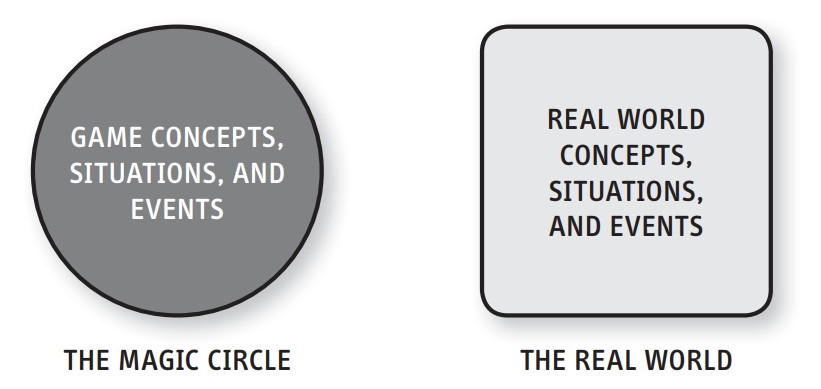
\includegraphics[width=\textwidth]{./Pictures/res/fundamentals/magic-circle}
    \caption{Magic Circle~\cite{10.5555/2544002}}
    \label{fig:magic-circle}
\end{figure}
\\
\textbf{Goals} need to be set in order to correctly design and implement a game.
During the play-through, there always have to be objectives to the user.
Even though a game may seem very goalless, there may be some unseen goals such as acts of creativity / creation, which may also be
referred to as a goal.
\\
\textbf{Rules} instruct the player through the game and give a boundary or limit to the game.
They are used to describe allowed actions during the gameplay, define progression and - if applicable - give a condition to
end the game.
\\ \\
Generally, the definition of a game is very broad and there are different opinions on the definition, however most of them
do not refer to the games' purpose: it may be purely for entertainment, but can also be for studying, training or attracting interest
for a topic, which is especially the case in the scope of this work.

\subsection{Educational Games}\label{subsec:educational-games}
Most games have a certain factor of education, so called \textit{stealth-education} involved, even though not
specifically intended to be educational.
However, there exist also games with the specified purpose of education, this may include simulations, persuasive games,
games for studying and games that support health and growth.
Educational games are a sub-genre of the \textit{Serious Games}-genre and aim to present or solve real world problems,
while maintaining a factor of entertainment.
Different ways of presentation may be used for educational games~\cite[p.43]{10.5555/2544002}.
While this work mainly aims to attract interest for the topic of aircraft system engineering in a fun and entertaining way, it is still
referred to as an education game in this context, as a definitive, wanted and positive side effect of playing the game is
to introduce the user to basic concepts of system design.
This can be seen as the underlying educational problem and challenge, since the borderline of serious games and games solely
for entertainment purposes is relatively non-restrictive.

\subsection{Game Development Stages}\label{subsec:game-design-stages}
There is no unanimous definition of the game development process, however most approaches and perspectives are similar and the different
stages can be categorized as three main stages~\cite{cg:game-design-stages}:
\begin{enumerate}
    \item Pre-production~\ref{subsubsec:pre-production}
    \item Production~\ref{subsubsec:production}
    \item Post-production~\ref{subsubsec:post-production}
\end{enumerate}
During these stages, different tasks and goals have to be accomplished and reiterated, which will be broken down in detail in the chapters below.
By using the digital educational game life cycle~\ref{fig:deglc} by Aslan and Balci, each of the three stages will be placed in context of
educational games specifically.
\begin{figure}
    \centering
    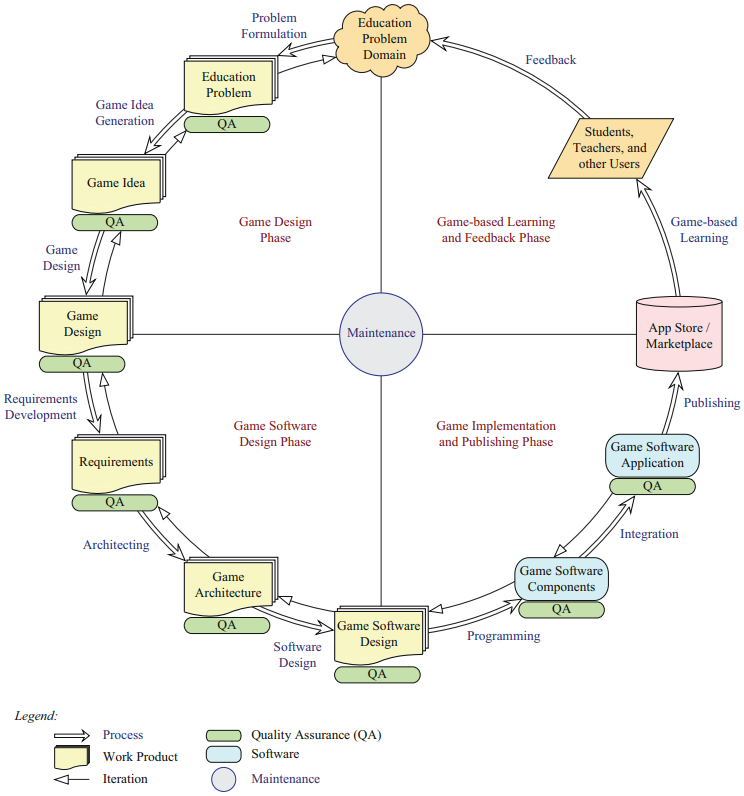
\includegraphics[width=\textwidth]{Pictures/res/fundamentals/deglc}
    \caption{Digital educational game life cycle~\cite{GAMED}}
    \label{fig:deglc}
\end{figure}

\subsubsection{Pre-production}\label{subsubsec:pre-production}
Pre-production is the development stage where only few code is written and the focus lies mostly on defining
problems, laying out ideas and prototyping.
Some important questions have to be answered during the pre-production stage, which are necessary to
head into production and development of the game.
The asked questions focus on the game subject, audience, resources needed and an estimated timespan, as well as
defining the four major elements of a game, as described in~\ref{subsec:game-definition}.
Sketches and concept art is designed and often, a prototype is developed.
At this stage, when the project team notices flaws or generally bad ideas, game development is either discontinued or the idea and concepts are
reiterated.
The process of pre-production can range in a timespan of a week to multiple months, depending on the size of the project and
the team~\cite{cg:game-design-stages}.
\\
As seen in~\ref{fig:deglc}, the first stages in the cycle of educational game development represent the idea of a pre-production stage fairly well,
as the main focus is to define the educational problem or subject that has to be solved or taught and why it would be more effective
to do so using a game approach.
Furthermore, requirements to the game and possible approaches to architecture and software design are defined and reiterated.
Note, that even during the next stages, there may be reiterations going back to a previous phase or stage.\ref{GAMED}.
\\
The notable products of the pre-production stage are concepts, ideas, design choices and in the case of educational games an approach to solving and identifying
an existing problem;
and a possible prototype of the idea.

\subsubsection{Production}\label{subsubsec:production}
Going into production, the defined idea is developed and code is produced.
Programming best practices are advised to be implemented during the coding process, as it improves maintainability.
Among these are well-named variables, classes and methods according to the programming language standards, code documentation (e.g.\ javadoc) and code formatting.
The game framework, engine and components to successfully set up the game are programmed.
Professional game productions include different milestones during this phase.
Past prototyping, the first milestone is the first playable game, which should give a better idea of the gameplay and graphic design.
Placeholders should be replaced by actual graphics.
After that, a pitch-able project is finished, which is fully payable and provides some better insight.
This is called a vertical slice.
The actual generation of content, e.g. levels, characters, etc.\ are integrated into the game during
pre-alpha.
While in pre-alpha the game features are still developed, in the alpha stage of the game it is finished in a sense, that is fully playable from the beginning
until the end.
At this point, the major objective is testing and bugfixing.
During the beta, content creation is completely finished and no new features are added - the focus is on optimizing what is available instead of
changing or adding new things.
The final state of the game, which should also be the end of production stage, is a finished game, which is fully playable and can be
released and used to and by the public~\cite{cg:game-design-stages}.
\\
At the end of the production stage, the framework is clearly laid out and well documented, as well as the game itself is finished for publication~\cite{GAMED}.

\subsubsection{Post-production}\label{subsubsec:post-production}
The post-production stage mainly focuses on maintenance, patches and bug fixes to the finished game, as there are more people playing and therefore more bugs
are found.
Feedback is given to the developers, which may be implemented in future projects.
Usually, this ends the game development process, as there are no new added features (except DLCs - downloadable content, or other add-ons) to the game anymore~\cite{cg:game-design-stages}.
In the case of learning focused or educational games, there may be more iterations of the process, which take the feedback and results of the project into
consideration and develop a new, revised version of the application~\cite{GAMED}.

\subsection{Game Engines}\label{subsec:game-engines}
Game engines are software frameworks that game developers use to create video games more efficiently.
They provide a set of tools and features that allow developers to create games without needing to build everything from scratch.
Game engines typically provide a range of features, including graphics rendering, physics simulation, audio processing, animation, scripting, and networking.
\\
Game engines come in various forms, from open-source engines that can be freely used and modified by anyone, to commercial engines that require a license fee to use.
Some examples of popular game engines include Unity, Unreal Engine and CryEngine.
\\
Game engines can help reduce the time and cost of game development by providing pre-built components and tools, allowing developers to focus on creating the game's content and gameplay mechanics instead of building the underlying technology.
Additionally, game engines can make it easier to create games that run on multiple platforms, such as desktop computers, mobile devices, and gaming consoles, by providing cross-platform support.
\\
Game engines have become an essential part of the game development process, and have helped democratize game development by making it more accessible to independent developers and small studios.
\\
The above-mentioned game engines use different approaches and concepts, which are pointed out here to give an overview over the generally possible approaches to
designing and developing game engines.
Generally, game engines are developed in high level languages, e.g.~C\#, Java or C++, the reason being object-oriented programming,
which allows general concepts such as inheritance, polymorphism, encapsulation and abstraction to create reusable, maintainable and modular code.
\\
\subsubsection{Unity}\label{subsubsec:entity-component-system}
For the unity engine, a generic entity component system (ECS) design pattern is used, as seen in figure~\ref{fig:ecs-unity}.
The basic idea behind using an ECS is to separate object data and behavior into components, respectively systems.
Each entity is a unique identifier for an object within the game, this can be anything from a button to a sound.
Entities consist of a variety of components, while each entity can have different components based on the needs.
A purely graphical entity which shows an image may only consist of a single graphics component, however another entity may contain
a component for graphics, one for sound and another one that holds collision information.
It is important to note, that components never change an entities' behavior, but only contain data that describes the entity.
Systems are responsible for collecting all relevant entities (i.e.\ entities that contain specific components) and processing them.
An example for a system is a rendering engine, which collects all graphical entities \& components and renders them to the screen by
using the data that is stored within the respective graphics components.
\\
Entity-Component-System approaches may also be used paired with other approaches of game design and are generally very broadly customizable and adaptable
to specific needs of the developer.
\begin{figure}
    \centering
    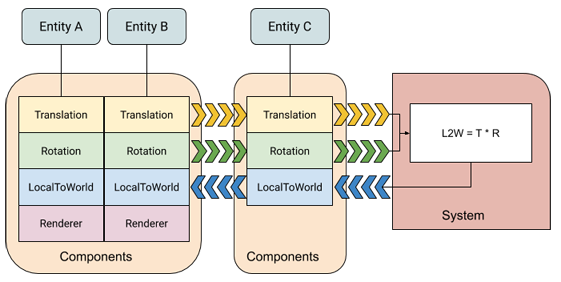
\includegraphics[width=\textwidth]{Pictures/res/fundamentals/ECSBlockDiagram-unity}
    \caption{ECS System used by the Unity Engine \todo{add cite}}
    \label{fig:ecs-unity}
\end{figure}
\subsubsection{Unreal}\label{subsubsec:unreal:-component-based-architecture}
Unreal Engine does not use an Entity Component System (ECS) in the same way Unity does with its Data-Oriented Technology Stack (DOTS) and ECS implementation.
However, Unreal Engine does use a component-based architecture, which shares some similarities with an ECS.
\\
In Unreal Engine, as seen in figure~\ref{fig:unreal-concept}, game objects are represented as Actors, which can have
various components attached to them to define their behavior and appearance.
This approach allows for modularity and reusability of code, which is one of the primary goals of an ECS.
\\
While Unreal Engine's component-based architecture has some similarities with an ECS, it does not follow the strict separation of
data and logic that characterizes an ECS. In an ECS, entities are simple identifiers, components hold only data, and systems
handle the processing of component data.
This separation of concerns allows for better performance and scalability, particularly on modern hardware with multiple cores, due to the possibility
of separating different systems into multiple threads.
\\
Unreal Engine's component-based architecture, though not a pure ECS implementation, provides a powerful
and flexible way to create game objects and manage their behavior.
This is done by a method which constantly updates each component by using their built-in methods, instead of having different systems accessing and changing data within components.
Developers can still achieve good performance and scalability by carefully designing their code and taking
advantage of Unreal Engine's built-in multi-threading and optimization features.
\\
Furthermore, Unreal Engine has a built-in visual scripting system called Blueprints, which allows developers to create game logic without writing code.
This system enables artists, designers, and programmers to collaborate more efficiently and helps those with little programming experience to contribute
to game development.
\begin{figure}
    \centering
    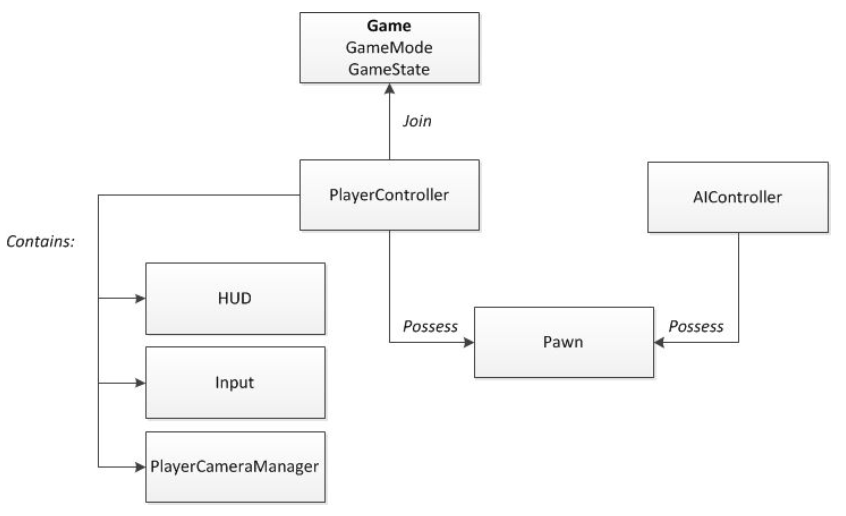
\includegraphics[width=\textwidth]{Pictures/res/fundamentals/unreal-framework}
    \caption{Unreal Architecture~\cite{UNREAL:Framework}}
    \label{fig:unreal-concept}
\end{figure}
\subsubsection{CryEngine}\label{subsubsec:cryengine}
While CryEngine mainly features the same patterns and approaches as Unreal does, one major standout is the very high fidelity graphical rendering
ability.
Particularly real-time rendering and physical based rendering underline this major benefit of using CryEngine, as it enables
creators and designers to create highly realistic environments, for example seen in games like Far Cry, made by Crytek using their own
engine.


\section{Problem}\label{sec:problem}
\todo{move to introduction?}
The subject of aircraft system design, particularly the concepts of redundancy, can be quite challenging to present and visualize
in an accessible and comprehensive way.
To address this, it is proposed that a gamified simulation be designed, developed, and implemented to make the material
more engaging and approachable.
\\
This interactive game is primarily aimed at young children, as well as primary and secondary school students.
It is intended to serve as an educational tool that can be employed during open-house events or as a means of
introducing the subject to individuals with little or no prior knowledge of the topic.
\\
Given that the game is designed to be playable at events such as industry fairs or open-house days,
it should be compatible with external gamepads, including game controllers.
The implementation should involve the use of a game engine to handle the calculations of logic and inputs.
Additionally, a variety of levels should be developed to effectively explain key concepts such as redundancy, common mode failures, and common cause failures.
\\
The ultimate objective is to provide an enjoyable, interactive visual representation of aircraft system engineering concepts,
while offering direct feedback to facilitate learning.
Players should be able to progress through the levels, experiencing a gradual learning curve that helps them grasp and
retain the concepts presented.

\section{State of the Art}\label{sec:state-of-the-art}
In the 21st century, e-learning has seen increasing implementation and adoption across various educational levels.
This includes the use of educational games and the integration of game-based learning methods not only in
high schools and universities but also in middle and elementary schools.
One major advantage of using games for educational purposes is that they enable students to experiment,
develop problem-solving skills, and gain a deeper understanding of decision-making processes,
all while receiving immediate visual or auditory feedback~\cite{application-of-education-games-to-enhance-student-learning}.
This is in contrast to traditional learning methods, such as writing essays or submitting homework,
which typically involve delayed feedback~\cite{more-than-just-fun-and-games}.
\\
Furthermore, learning through games can enhance motivation, attention, and retention while offering a flexible learning environment
in terms of both time and location.
However, it is worth noting that students often gravitate towards casual gaming over educational games.
This highlights the need to create engaging and interactive games that are both entertaining and educational to
effectively serve their intended purpose~\cite{WHITTON}.

According to Cheung and Ng~\cite{application-of-education-games-to-enhance-student-learning}, multiple studies in high schools and primary or secondary schools have found that educational
games are more likely to be integrated into the classroom by teachers of higher grades.
Younger learners, who are often more prone to inattention, can particularly benefit from
educational games, as these tools can help improve their attention span and overall learning experience.
\\
This presents an opportunity for the proposed work, which is specifically designed for younger age groups, to make the highly
technical subject of system engineering and redundancy concepts more accessible and engaging through a visual and interactive format.

\section{Science Day - University of Stuttgart}\label{sec:science-day---university-of-stuttgart}
The ``Tag der Wissenschaft'' (Science Day) is an open-door day, where the University of Stuttgart can be experienced by everyone.
Exhibits, research environments and results, laboratories and more can be seen, tested and used by everyone, including families, younger children,
high-school students, etc.
It is supposed to show recent research topics and provide insight into the actual work done at a university, while also providing insights
into different studies for interested people who may want to start their studies at the University of Stuttgart ~\cite{tag-der-wissenschaft}.
% Identification of safety critical system components?
% Definition of simulation requirements & constraints
% Gamification strategy: what should the objective be, how should the user be engaged -> use the definition of Game to point this out
% Conceptual Design of Game Engine (Architecture & Features)
% Conceptual design of scenes / characters / challenges (goals, visual elements, structure)
% validation method used

\chapter{Conceptualization}\label{ch:design}
In this chapter, the game idea is presented.
All major elements of the game design process are defined and explained and requirements and constraints to the game are detailed, as well as
the structure of the framework of the game engine is described.

\section{Requirements}\label{sec:requirements}
As the major objective of the game was to create a fun environment for users to test and familiarize themselves with the topic of
aircraft system design and different architectures used, the game requirements can be defined.
\\
The game should introduce users to the concepts of redundancy and system failures, as well as different failure types such
as common-mode and common-cause failures.
The game has to have a good mix of fun and interactivity, while the sole purpose should not be entertainment, but rather a
mix of entertainment and education.
Education, in this context, is referred to as the part of awaking interest for a rather unknown topic.
Therefore, the game should be playable without any kind of knowledge regarding the topic of aircraft systems and should be easy
to get into.
Explanations and details should only be given as an addition, however should not be directly necessary to understand the basic concept
of gameplay.
It should be playable on open-door days, where it is not as pleasant to play the game only with mouse and keyboard, therefore a game pad
integration is necessary.

\section{Genre}\label{sec:genre}
The \textit{Puzzle} genre is chosen for the graphical user interface and interaction, while the major calculations for the
games' content may be categorized as \textit{Simulation}, however not much of the actual simulation is visible to the player.

\section{Game Engine Design}\label{sec:game-engine-design}
In this section, an overview of the game engine architecture and core features is given.
The design principles and development methodologies are clarified and challenges regarding the implementation will be defined.

\subsection{Architecture}\label{subsec:architecture}
The game engine uses an entity component system approach, which aims to decompose the game objects (entities) into small, reusable and interchangeable
components, that act as simple data containers to define properties of an object.
The game engine follows an object-oriented programming approach, where entities and components are designed to be easily extendable and inheritable.
This allows for an easy creation of new types of entities or components by reusing and extending existing ones, without modifying the core engine code.
To achieve this, a set of base classes for entities, components and systems is defined, which can be subclassed and implemented to provide the custom data and
properties and logics needed.
Components should simply act as data containers, which also follows the data encapsulation approach typically used in object-oriented programming, as
the interface to access the data within a component is provided by the components' getter and setter methods.
The game engine follows a modular approach, where a set of systems - which is either pre-defined by the core game engine (e.g.\ rendering, sounds) or
a custom implementation by the game - is executed by a game loop to handle inputs, game logics and updates to the entities and components.
This modular approach allows for an easy addition or removal of systems depending on the game implementation, without affecting the game loop.
This also enables for optimizations such as parallelization of the execution of the systems, which leads to performance and scalability improvements.
However, in the scope of this thesis, it may not be necessary to parallelize the game systems.

\subsection{Features}\label{subsec:features}
The core features provided by the game engine are rendering, audio handling, input handling, resource management and language management.
\\
The rendering system provides handling of different screen dimensions, options for fullscreen visualization and window mode, and allows
for rendering of different graphical objects, such as text, shapes, images or animations.
Rendering is done solely in 2D and is based on the usage of the java built-in rendering system Graphics2D, which already provides a
variety of methods to help with the rendering process.
The rendering system also provides a scaling engine, which is used to correctly detect the actual screen position against the design point (e.g.\ a
game may be developed for 1920x1080px screens, but can also be used on other screen sizes).
\\
The audio system enables the game engine to play and mix different types of sounds and music with a support for different audio formats and codecs.
It is able to handle looped audios and helps in creating and enhancing the game environment.
\\
The game engine provides a flexible input system that allows to capture a variety of user inputs, including keyboards, mouse and gamepad events.
The input system supports a customization of different key bindings to functions, as it serves as a queue of events happening during the game which
may then be processed by other systems.
\\
Resource management is a built-in feature of the game which enables the developer to easily load different file types, such as images or XML files.
This includes languages, tile sets, high score files and level files of a pre-defined format.
The resource manager may be replaced with a custom resource loader, depending on the games' needs and requirements.
\\
A major part of the game engine is the handling of text within games, as text is represented by ids which are loaded from different language files.
This enables a support for different languages within the game without having to rewrite game code.
Language files may be translated to other languages and simply included to the game, where the user may switch the language.
A language management system which is based on using IDs (tags) instead of the actual text for any text string is used.
A processor is parsing all available language files in XML format and a look-up table that maps each ID to the corresponding text string is created.
Within the Rendering Engine, each text is rendered in the language the game is set to.

\section{Game Environment Design}\label{sec:game-environment-design}
Before implementing the game itself, a concept and idea for the game was developed and a prototype was built, which was refined during the
actual implementation process of the game.
In this chapter, the process of conceptualizing and designing the game, including mechanics and gameplay, graphic concepts and
level design is explained.

\subsection{Intended Gameplay}\label{subsec:intended-gameplay}
The player is playing an aircraft mechanic, who is supposed to investigate systems for possible failures and improve the given systems or
build new systems according to given requirements.
The player is given instructions by an aircraft engineer and a tablet device with some applications to show necessary
information, requirements and tips.
There are multiple levels with advancing difficulty that may be played.
Each of these levels shows and conveys different concepts used in system engineering.
To solve the puzzle levels, the user has different components to choose from in the inventory (also called the build panel), that
can be added to the current system configuration by drag and drop.
Components can be connected by using cables and putting them in the correct places and rotations.
As the game is grid-based, there are limited possibilities which have to be considered in level design, however most levels
may be solved in different ways, which are to some degree more or less efficient.
This is represented by the score that is calculated at the end of each level after validating the systems correct functionality, which gives
a hint to the player where he or she may perform better in order to score higher.
\\
The detailed game mechanics are described in the next section~\ref{subsec:game-mechanics}.

\subsection{Game Mechanics}\label{subsec:game-mechanics}
As the general intended game play was already stated in the previous chapter, the detailed game mechanics are going to be described in this section.
In each level, a defined set of components is already available on the game grid, which may or may not be replaceable, depending on the given
information from the level file.
\\
Each component has defined simulation parameters such as failure probability and failure detection rate, which can not be changed by the user.
Another set of components is added to the users build panel in each level, where they can be placed by drag and drop to the game grid.
The goal is to use the given space on the grid efficiently and build a system that has a failure ratio below the requirement / goal target failure ratio.
Components can be connected by using different cables (red, blue, green, yellow), which simply represent different layers of cables, so multiple
cables can be placed on a single grid tile.
Cables can be rotated to correctly connect components or cables of the same type.
Each cable port type color is also shown on the component itself to make clear, which components have in- and outgoing cable ports
that cables may be connected to.
\\
After setting up the system configuration, the player can start a simulation.
This simulation calculates the markov chain of the given system and adds up the failure probability of all states that lead to a system failure with the given
input requirements.
\\
Comparing this result to the goal leads to a passed or failed level, however the distance from the players' system to the target also matters when it comes to calculating
the score, which consists of exactly this distance, the remaining components in the players inventory and a base score for each level.
During the simulation process, the aircraft starts flying through the sky to give a visualization that something is happening, as with increasing
level size the time to calculate the probabilities rises accordingly.
\\
When the level is passed successfully, a visualization of that is given by showing a score board and fireworks, when the level is failed, the aircraft
shows explosions instead.

\subsection{Graphic Design}\label{subsec:graphic-design}
The goal of the graphic design process was to conceptualize the general layout of the game environment as well as the look and feel
of the major components used.
During this process, placeholders where used in a prototype game to visualize the placement of different UI and game elements.
The graphics design process was iterative and most graphics have changed frequently throughout the game development process.
Generally, due to the requirement to keep the game relatively simple to pick up for the target audience, it was chosen to keep
the graphics design simple and clean as well.
Therefore, a classical 8-bit graphics style is chosen for all graphics of the game, including UI.
For that, a color palette of mostly bright colors and various different tones of gray is used across all graphics.
\\
The following figures show the general layout concept of the level
menu scene \ref{fig:level-menu-scene-concept} and the game scene~\ref{fig:game-scene-concept}.
\begin{figure}
    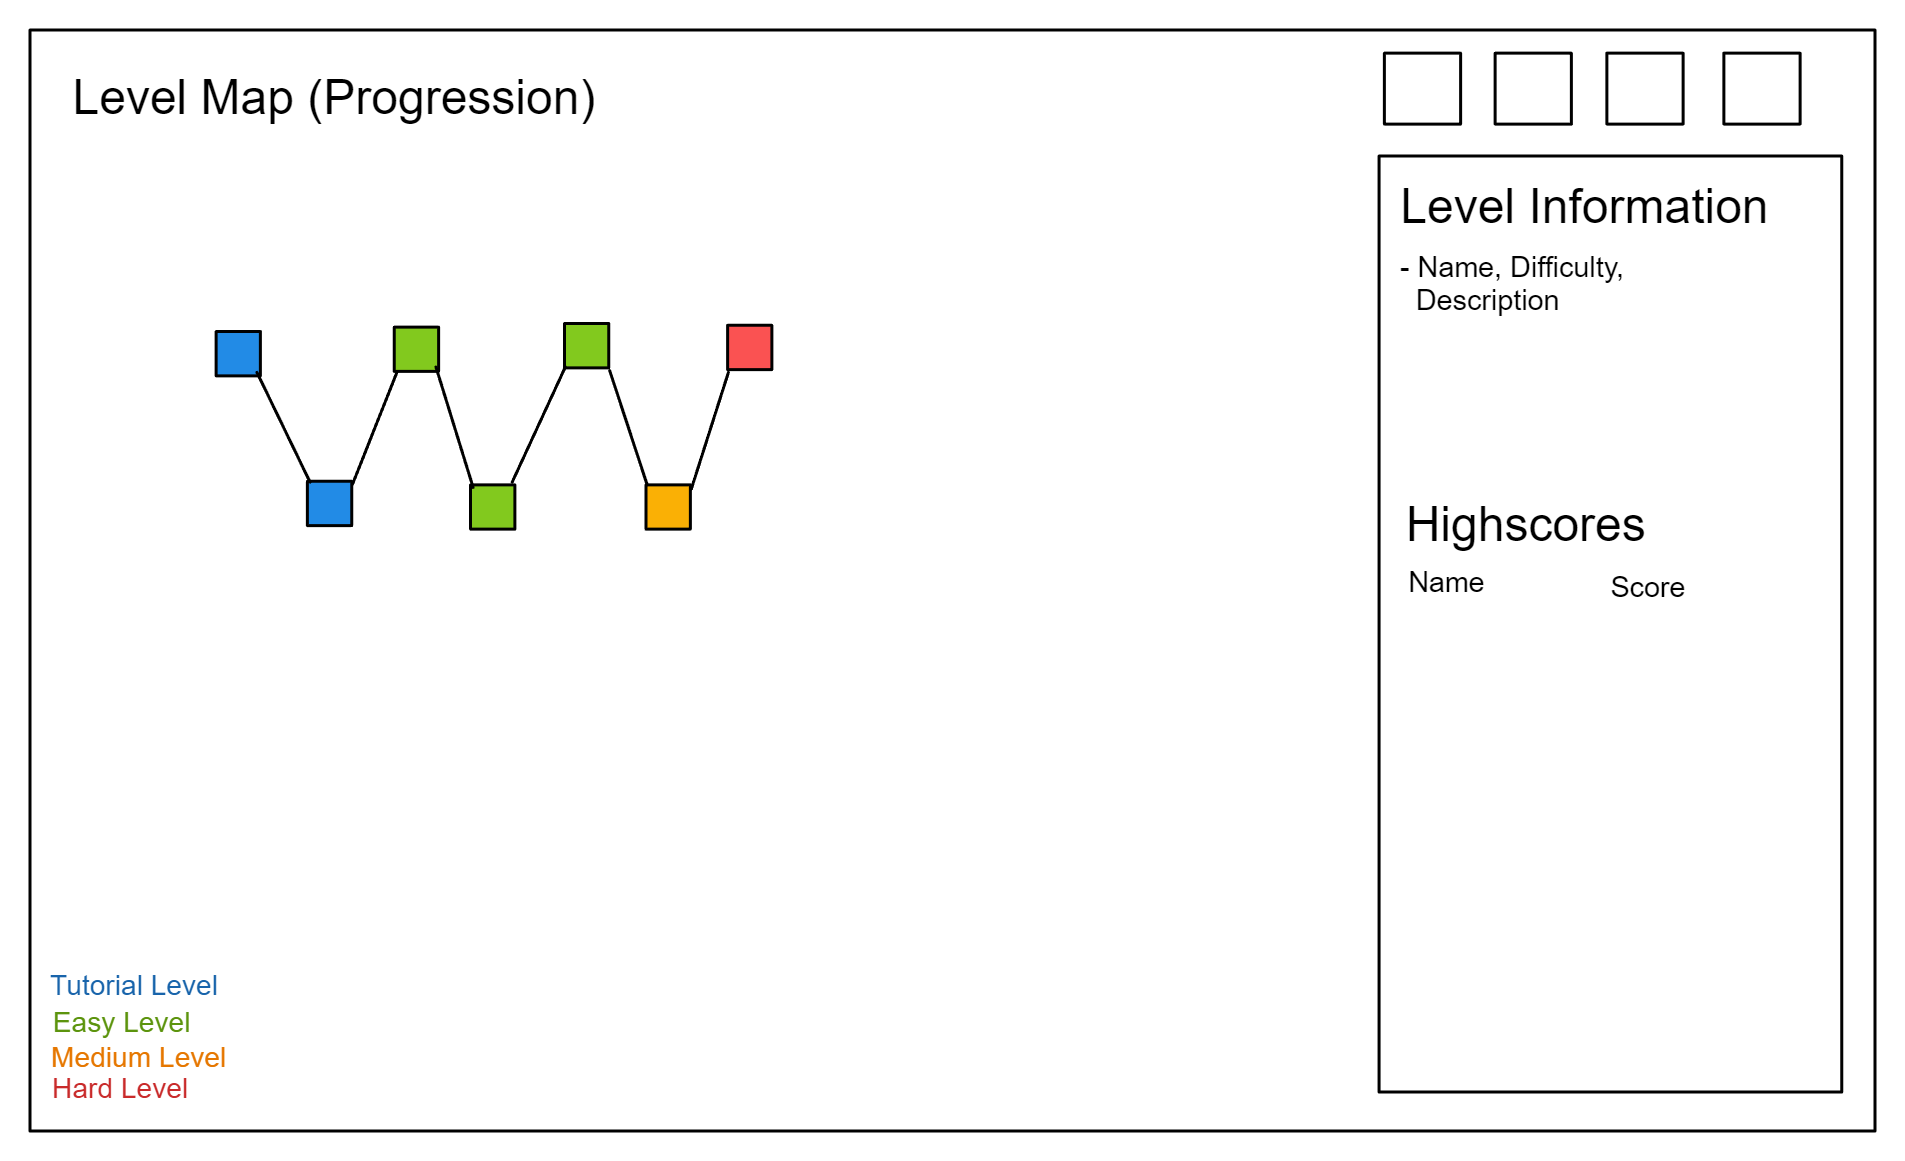
\includegraphics[width=\textwidth]{Pictures/res/concept/level-menu-scene-concept}
    \caption{Level menu scene concept}
    \label{fig:level-menu-scene-concept}
\end{figure}
\begin{figure}
    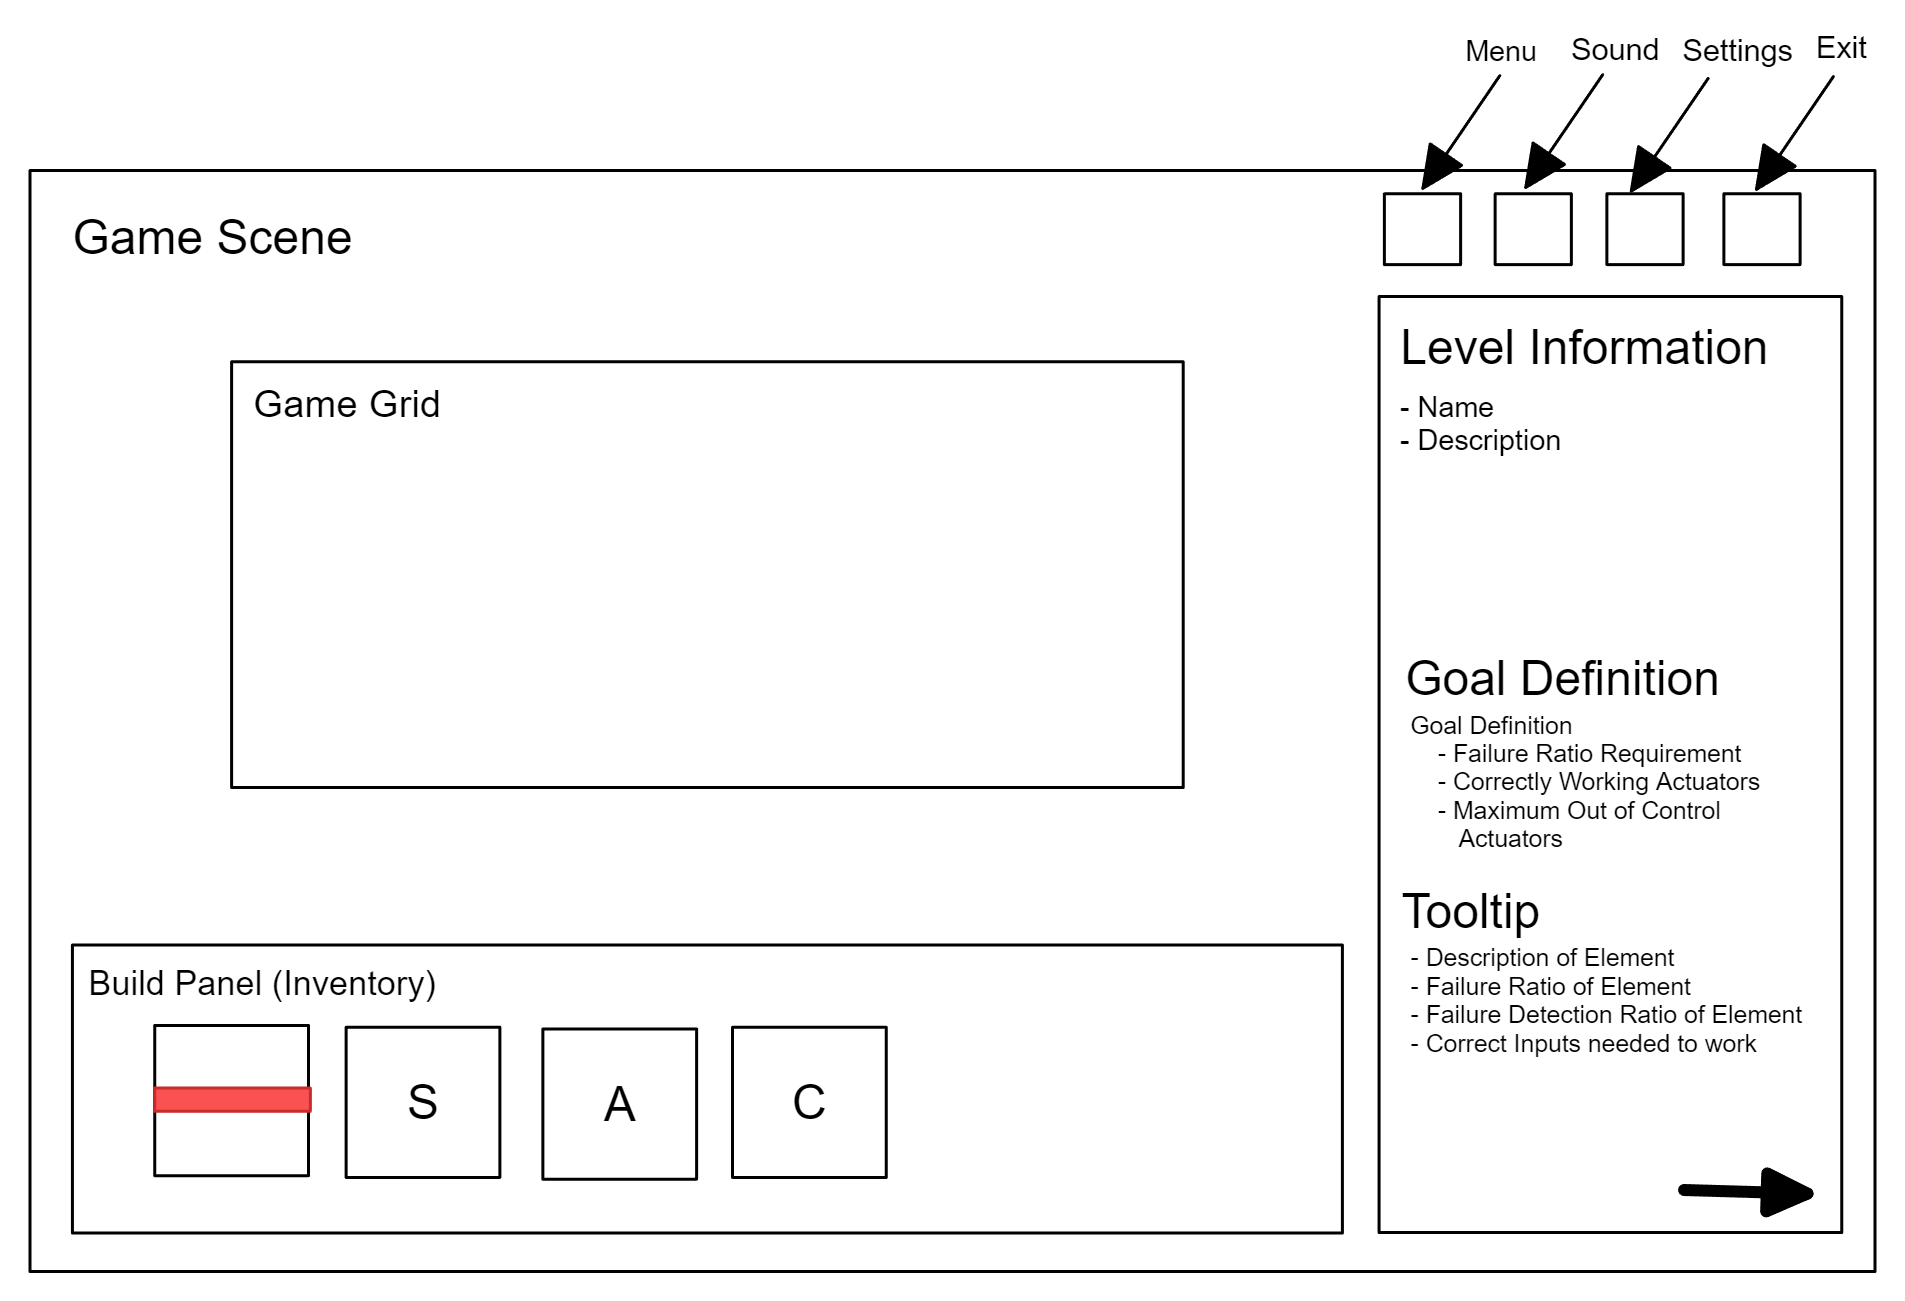
\includegraphics[width=\textwidth]{Pictures/res/concept/game-scene-concept}
    \caption{Game scene concept}
    \label{fig:game-scene-concept}
\end{figure}
According to the concept scene layouts, the following components have to be designed:
\begin{itemize}
    \item Screen backgrounds
    \item Background tiles, placeholder tiles
    \item Simulation components: actuators, sensors, computers, cables, \ldots
    \item Build panel
    \item Information panel
\end{itemize}

\subsection{Sound Design}\label{subsec:sound-design}
To provide atmosphere and create an 8 bit-styled experience, open source music will be used in the game.

\subsection{Level Design}\label{subsec:level-design}
The level design is a main part of this work, as the progression through the game and the process of explaining different concepts
within aircraft system design is heavily influenced by this.
Therefore, some levels were conceptualized before the implementation, to have a guideline for the actual implementation.
Levels are categorized in difficulties, reaching from tutorial to hard.
When passing a level, the user unlocks new levels to progress through the game, however the progression may be turned off and the user can choose from all
levels.
\\
Tutorials should guide the user through the features of this game and provide some insight on the basic gameplay and a general
understanding of aircraft systems, failures and redundancy concepts.
A visual representation of this is needed to provide enough input for younger age-groups to play and understand the game.
However, for other users, some more in-depth knowledge is also provided in order to better understand calculations, simulations and
game logic in the background.
Tutorial levels explain the basic usage, such as cable and component (re-)placement and the different safety requirement
categories.
\\
The categories are described by colors, from red (catastrophic) to blue (no safety effect).
Each component that can be built in the level also has this information to it, so the user can visually see a representation
of the criticality and the effect of the objects to the system and its requirements.
Each level goal is defined by a safety requirement and a minimum count of correctly operating actuators (or other components, such
as flight control computers, sensors, \ldots).
As the user progresses through the levels, there will be harder goals in safety requirements that need to be solved by using
redundancy concepts or mechanisms such as voting.
As this work aims to explain most of the basic concepts, some levels should also take into consideration common-mode and common-cause
failures.
\\
The following levels have been conceptualized for this game by default:
\begin{enumerate}
    \item Tutorials to explain basic game concept and system engineering concepts
    \item Duplex Systems with and without cross-strapping
    \item Triplex Systems
    \item Systems with multiple actuators
    \item Systems with duplex sensors
    \item Common-Mode Failure scenario
    \item Common-Cause Failure scenario
\end{enumerate}
Each level has a defined goal, that has to be achieved in order to pass the level.
Tutorials aim to explain the basic concepts of gameplay and systems, such as placing components, connecting and rotating cables and
explaining the difference between out of control and passive failures, failure probability, failure detection ratio / integrity and the purpose
of different components that may be used to complete the levels.
\\
During the conceptualization, high-level designs for each level, including layouts, objectives and possible additional content were created.
Sketches and visualizations of the level ideas helped to create a baseline for the implementation that was used later during development of the levels.
During the implementation and production process of the game, most of the level designs were revised and adjustments were made, which is also
an iterative task where updates may be needed in the future.
\\
The finalized level designs and implementations will be shown in section~\ref{subsec:level-implementation}.
\\
Additionally, through a build mode the user is able to set up new levels including the requirements / level goal via the built-in
frontend, which then saves the level to a new xml file.

\subsection{Tutorials}\label{subsec:tutorials}
As some text is necessary to correctly explain the gameplay and concepts such as redundancy, characters are designed in order to create
a dialogue with the player to make the experience, even though reading is an essential part of the game, more user-friendly and interactive.
The characters available to the game, which appear whenever dialogues and tutorials should be shown, are the character representing the user, who is displayed
as an aircraft mechanic who has to repair and investigate different systems in the aircraft and another character who gives the user instructions and
leads the user through the game, who is an aircraft systems engineer.

\subsection{Language}\label{subsec:language}
As the game is supposed to be used by a broad audience, especially in Germany and at the University Day of the University of Stuttgart, there should be an option
to change the language.
Therefore, english, german and a simplified version of the german text file are supported by default.
% Development of game engine - core components & functonalities
% development of game using the game engine, including level/scene design (asset creation, scene scripting & interaction, development in general)
% UI / XP Design
% Testing & Debugging (Test cases / scenarios), (Logging, Debugger, Code Analysis), Performance Testing (-> memoization, ...), playtesting?

\chapter{Development \& Implementation}\label{ch:implementation}
In this chapter, the implementation of the game engine including the basic framework, graphic rendering and input handling is described.
The game is implemented by using the game engine framework and its features as a baseline which is extended to the game requirements and goals
defined in the previous chapters.
The game mechanics are developed and programmed in line with the entity-component system approach, as well as the Markov process is explained.
Furthermore, important scene and graphics designs are described as this is integral to understanding the implementation.

\section{General Approach}\label{sec:general-approach}
The game engine is implemented as a separate, independent, enhanceable framework, which may also be used to design other
games.
It provides basic functionality for all features needed to design a game, such as input and system handling, rendering, configuration
classes and managers.
The implementation uses a basic entity-component-system as foundation and enhances this with further features.

\section{Programming Language}\label{sec:programming-language}
The programming language that was chosen for this implementation is \textit{JAVA}.
Java is a high-level, object-oriented programming language that was originally developed by Sun Microsystems (now owned by Oracle Corporation) in the mid-1990s.
It is designed to be portable, meaning that it can be run on a wide variety of platforms, including Windows, macOS,
Linux, and many others, without needing to be recompiled for each platform.
\\
Java is widely used for developing both desktop and web-based applications, as well as mobile applications for Android devices.
It is also used extensively in server-side programming and for building enterprise applications.
\\
One of the key features of Java is its virtual machine (VM), which allows Java programs to be executed on any system that has a compatible JVM installed, regardless of the underlying hardware and operating system.
This makes it possible to write a single Java program that can run on multiple platforms, without needing to be modified for each one.
\\
Java also has a large standard library of classes and functions, which makes it easier to write complex programs without needing to reinvent the wheel.
Additionally, Java is known for its strong emphasis on security, which makes it a popular choice for building applications that need to be highly secure
and resistant to cyber attacks.
\\
Java was chosen because of the wide variety of standard libraries and resources available, the very object-oriented programming approach which enables for
extending and inheriting of classes to adapt objects to the games and game engines needs.
Due to garbage collection, Java enables developing without having to consider memory allocations.
Furthermore, a great benefit of using Java is the multi-platform support due to Java being an interpreted language which works
independent of operating systems or processor architectures~\cite{JAVA}.

\section{Game Engine}\label{sec:game}
The game engine implements a variety of methods and classes which are used for handling the general program execution, independent of the actual game implementation.
In this chapter, these classes will be explained in detail and the general concept of the engine is reviewed.

\subsection{Entity Component System}\label{subsec:entity-component-system-implementation}
The entity component system setup used in this implementation can be approached from a top-down point of view, visualized in figure \ref{fig:ecs}.
A scene is the basic class that contains all information about the currently displayed entities and the handlers and systems to be used
in the background.
There exist multiple scenes of different classes, such as scenes for the game view, menu scenes etc., which can be created by
inheriting the base scene class.
Scenes can be added to the game by using the Scene Manager, which is also used to swap between available scenes.
Each scene contains a list of entities, that could be referred to as a database of all available objects.
Entities represent a combination of different data containers, so-called components, which can be uniquely attached to each entity.
There are some standard entities and components available directly via the engine, however there may be the need for more components and entities while implementing the actual game.
The design approach of this entity component system is similar to the Unity implementation, however some simplifications were made to guarantee ab easily maintainable
and highly customizable game engine, without having to rely on third parties to bring in needed updates.
Furthermore, the simplifications made help with keeping an overview of all features needed and decreases unused features, to keep the engine as non-complex as possible.
\begin{figure}
    \centering
    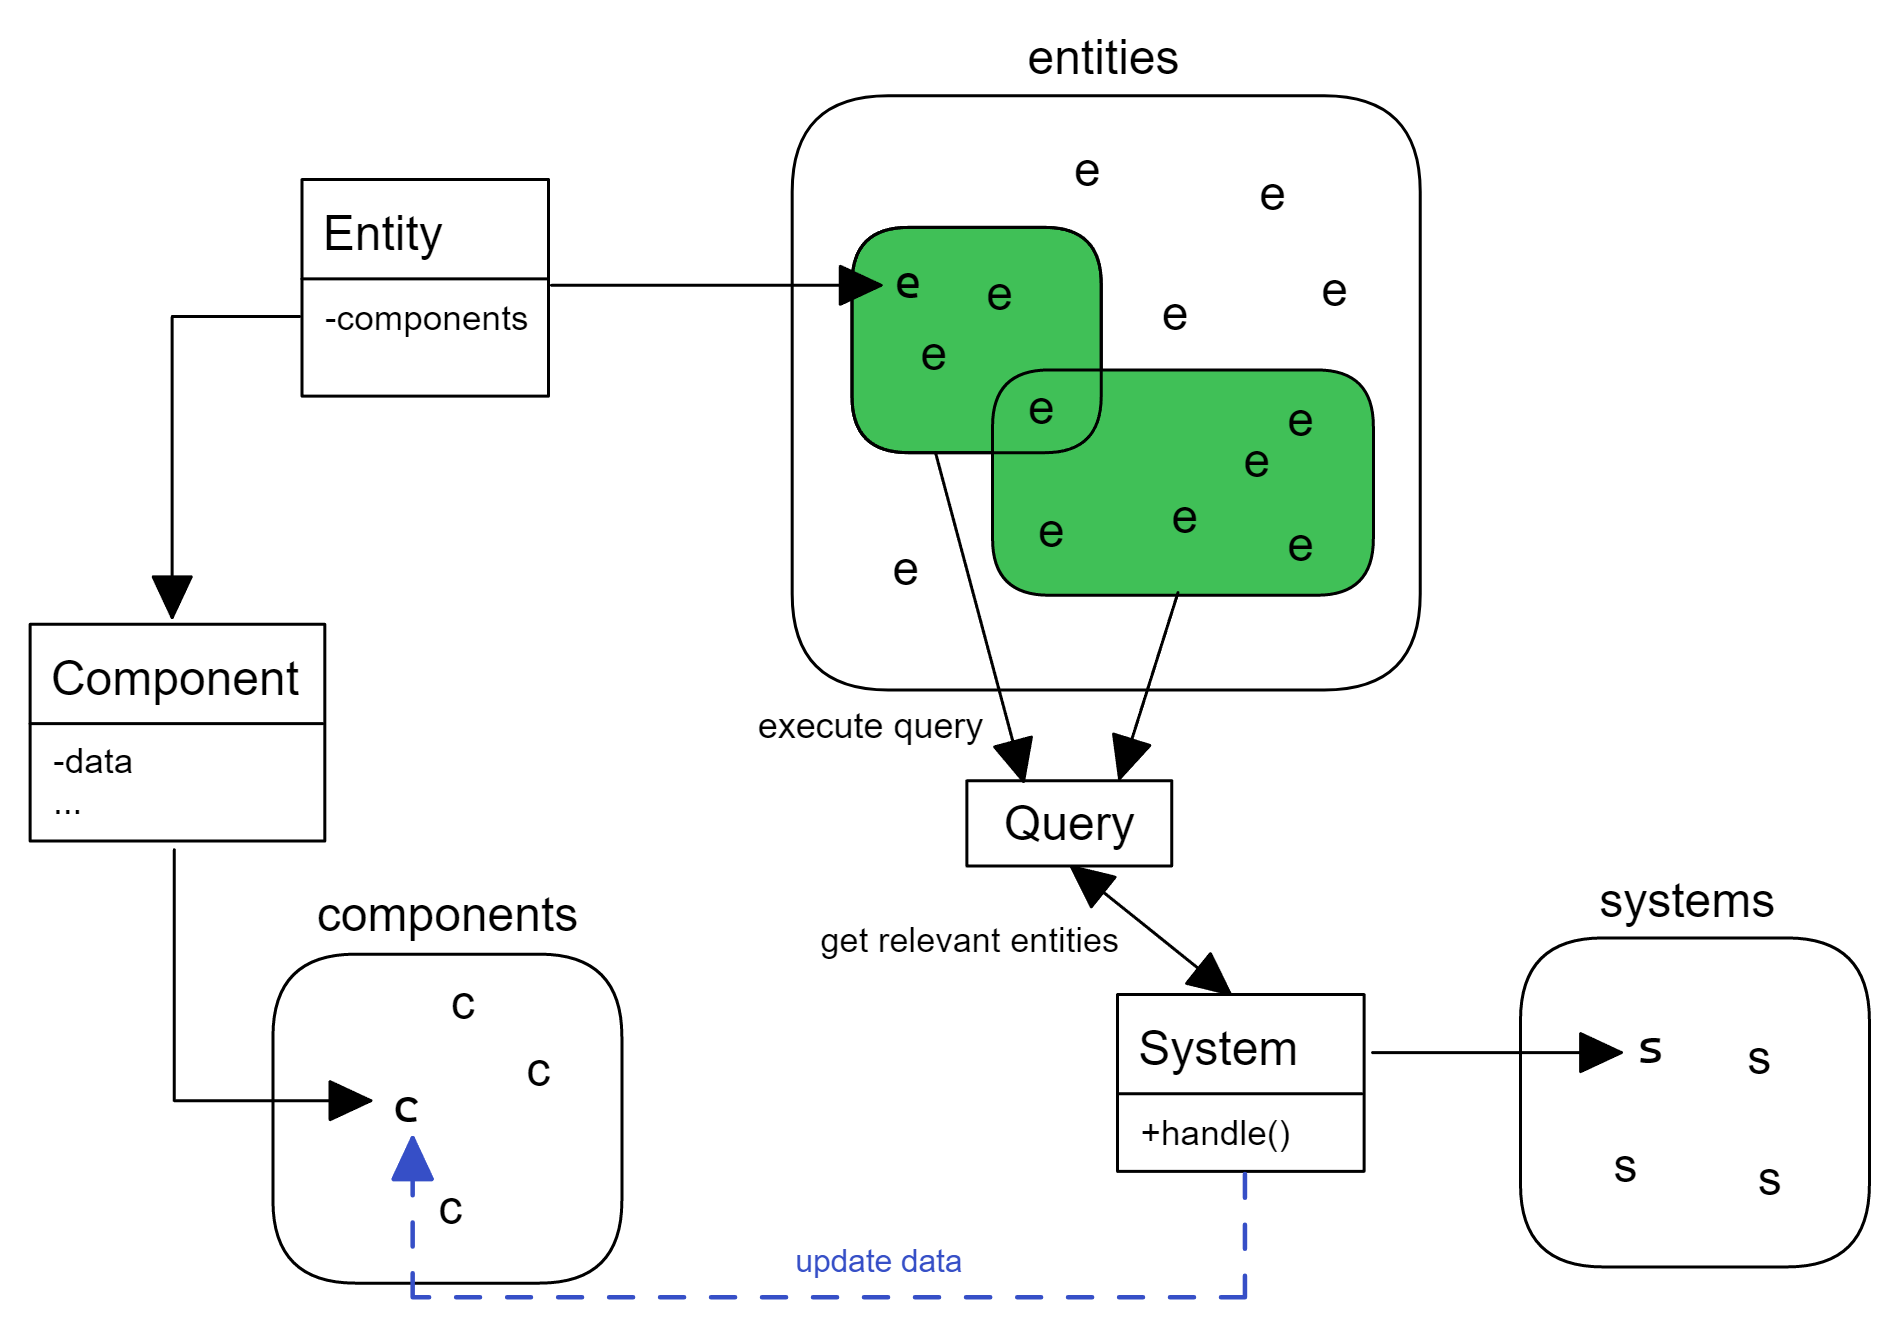
\includegraphics[width=\textwidth]{Pictures/res/implementation/ecs-database}
    \caption{ECS Database}
    \label{fig:ecs}
\end{figure}
\subsubsection{UML Diagram}\label{subsubsec:uml-diagram}
The UML diagram as seen in figure \ref{fig:ecs-block-diagram} shows a simplified structure of the engine implementation, which is going to be used to explain the mechanisms
and the framework of the implementation.
\begin{figure}
    \centering
    
\includegraphics[width=1.0\textwidth]{./Pictures/res/implementation/ecs-uml}
    \caption{Simplified UML diagram of the engine implementation}
    \label{fig:ecs-block-diagram}
\end{figure}

\subsubsection{Entities}\label{subsubsec:entities}
Entities are classes constructed from different, unique components, which could be referred to as containers storing different parameters to
describe the input behaviour of the systems.
Entities can not directly interact with each other, as any modification to data is strictly handled by the game engines' systems and handlers,
however components may contain direct references to other entities if needed.
The Entity class implements functions to add, remove and get Components of a class type.
\\
As there are usually lots of different types of entities in a game which may contain the same components, it makes sense to inherit from the Entity class and
build generic entities which can be reused.
For GUI elements, the game engine already provides some pre-designed entities, such as buttons, text bodies, panels and image entities.
During the implementation, it was chosen to handle GUI elements as entities as well, as the game engine is purely working in 2 dimensions and therefore
rendering methods for the game itself and the GUI do not differ.
This approach was the easy choice, as having a separate class to implement UI elements would most likely end up with a lot of duplicated
code fragments, which are already implemented in the RenderingComponent, as described in the next chapter.
\subsubsection{Components}\label{subsubsec:components}
All entities are built of a subset of the available components, uniquely attached to each.
The components available by default will be explained in detail in the following chapter.

\textbf{Render Component:} \\
The \textit{RenderComponent} class is designed to manage and store a diverse set of graphical objects that are utilized for
rendering various elements within a scene.
These graphical objects are categorized into subclasses, such as text, images, animations, hovering, lines, and shapes.
Each subclass is defined by a set of parameters that dictate its appearance, including aspects like location, bounds, colors,
images or animations, and text content.
\\
To address the need for rendering multiple graphical objects per entity while still adhering to the unique
component-per-entity constraint, the RenderComponent class allows for the addition of each graphical object multiple times.
For example, an image that requires occasional hovering may have one object to render the image itself, and
another object to render the hovering shape.
\\
Furthermore, the RenderComponent class incorporates methods that enable the retrieval of specific lists of
graphical object instances based on their corresponding class.
This functionality resembles the Query implementation found in the entity component system, providing a
streamlined and efficient way to access the desired graphical objects.

\textbf{ColliderComponent:} \\
Similar to the \textit{RenderComponent}, the \textit{ColliderComponent} also stores a list of collision objects, which are described by location and bounds.
Each of these collision objects is checked by the \textit{CollisionDetectionSystem} and handled accordingly, e.g.\
hovering an object at the same location as the collision object.

\textbf{Sound Component:} \\
The \textit{SoundComponent} class can be attached to any entity that needs to have a sound played at times.
It implements methods to set the state of the sound sample to play, pause or stop and contains the actual sound sample to be used by the \textit{SoundEngine}.

\textbf{Action Component:} \\
\textit{ActionComponents} are used for storing a mapping of input to action within an entity, e.g.\ clicking a button which opens another scene.
Each \textit{ActionComponent} is processed by the \textit{ActionSystem}.

\textbf{Cursor Component:} \\
The cursor component is a component used for handling game pad inputs and acts as a virtual mouse cursor, which can be moved by using
joysticks of game pads or keyboard buttons.
It simply indicates the position, where new mouse events are generated, when the actual mouse is not used.
\subsubsection{Scene}\label{subsubsec:scene}
A scene is a collection of entities that together form an aspect of the game, e.g.\ a menu or a level.
The \textit{Scene} class is an abstract class implementing methods for adding and removing entities from itself.
\\
To add a scene to the game, a scene object needs to be instantiated and added to the games' \textit{SceneManager}, where all
scenes are stored and the currently active scene can be set.
Generally, all systems access the scene manager to only process the currently active scene, or if needed handle entities in other scenes or add or remove them.
\subsubsection{Systems}\label{subsubsec:systems}
Systems are the third major part of the ECS implementation and handle any modification to the components.
They are used for a variety of different purposes and can be split into multiple sub systems, which each serve their own purpose.
The ECS implementation aims and encourages to split each function or feature into modular systems, which can then be added to the game where they
are handled within the \textit{GameLoop} as explained in section~\ref{subsec:game-loop}.
A variety of systems is already available per default, including rendering, collision and input systems, which will be explained in the following chapters.
\\
Each system queries through the available entities / components and only processes the relevant ones.
The query system is set up as a static class that can be accessed from anywhere.
It implements methods that can be used to search for all entities of a class or entities that have a specified component
attached to it within the currently displayed scene.
The set of entities can be seen as a database that is filtered by the query system to obtain only a subset with the specified component or class type, which may be used
for other systems.
System processing is shown in figure~\ref{fig:ecs-system-processing}.
\begin{figure}
    \centering
    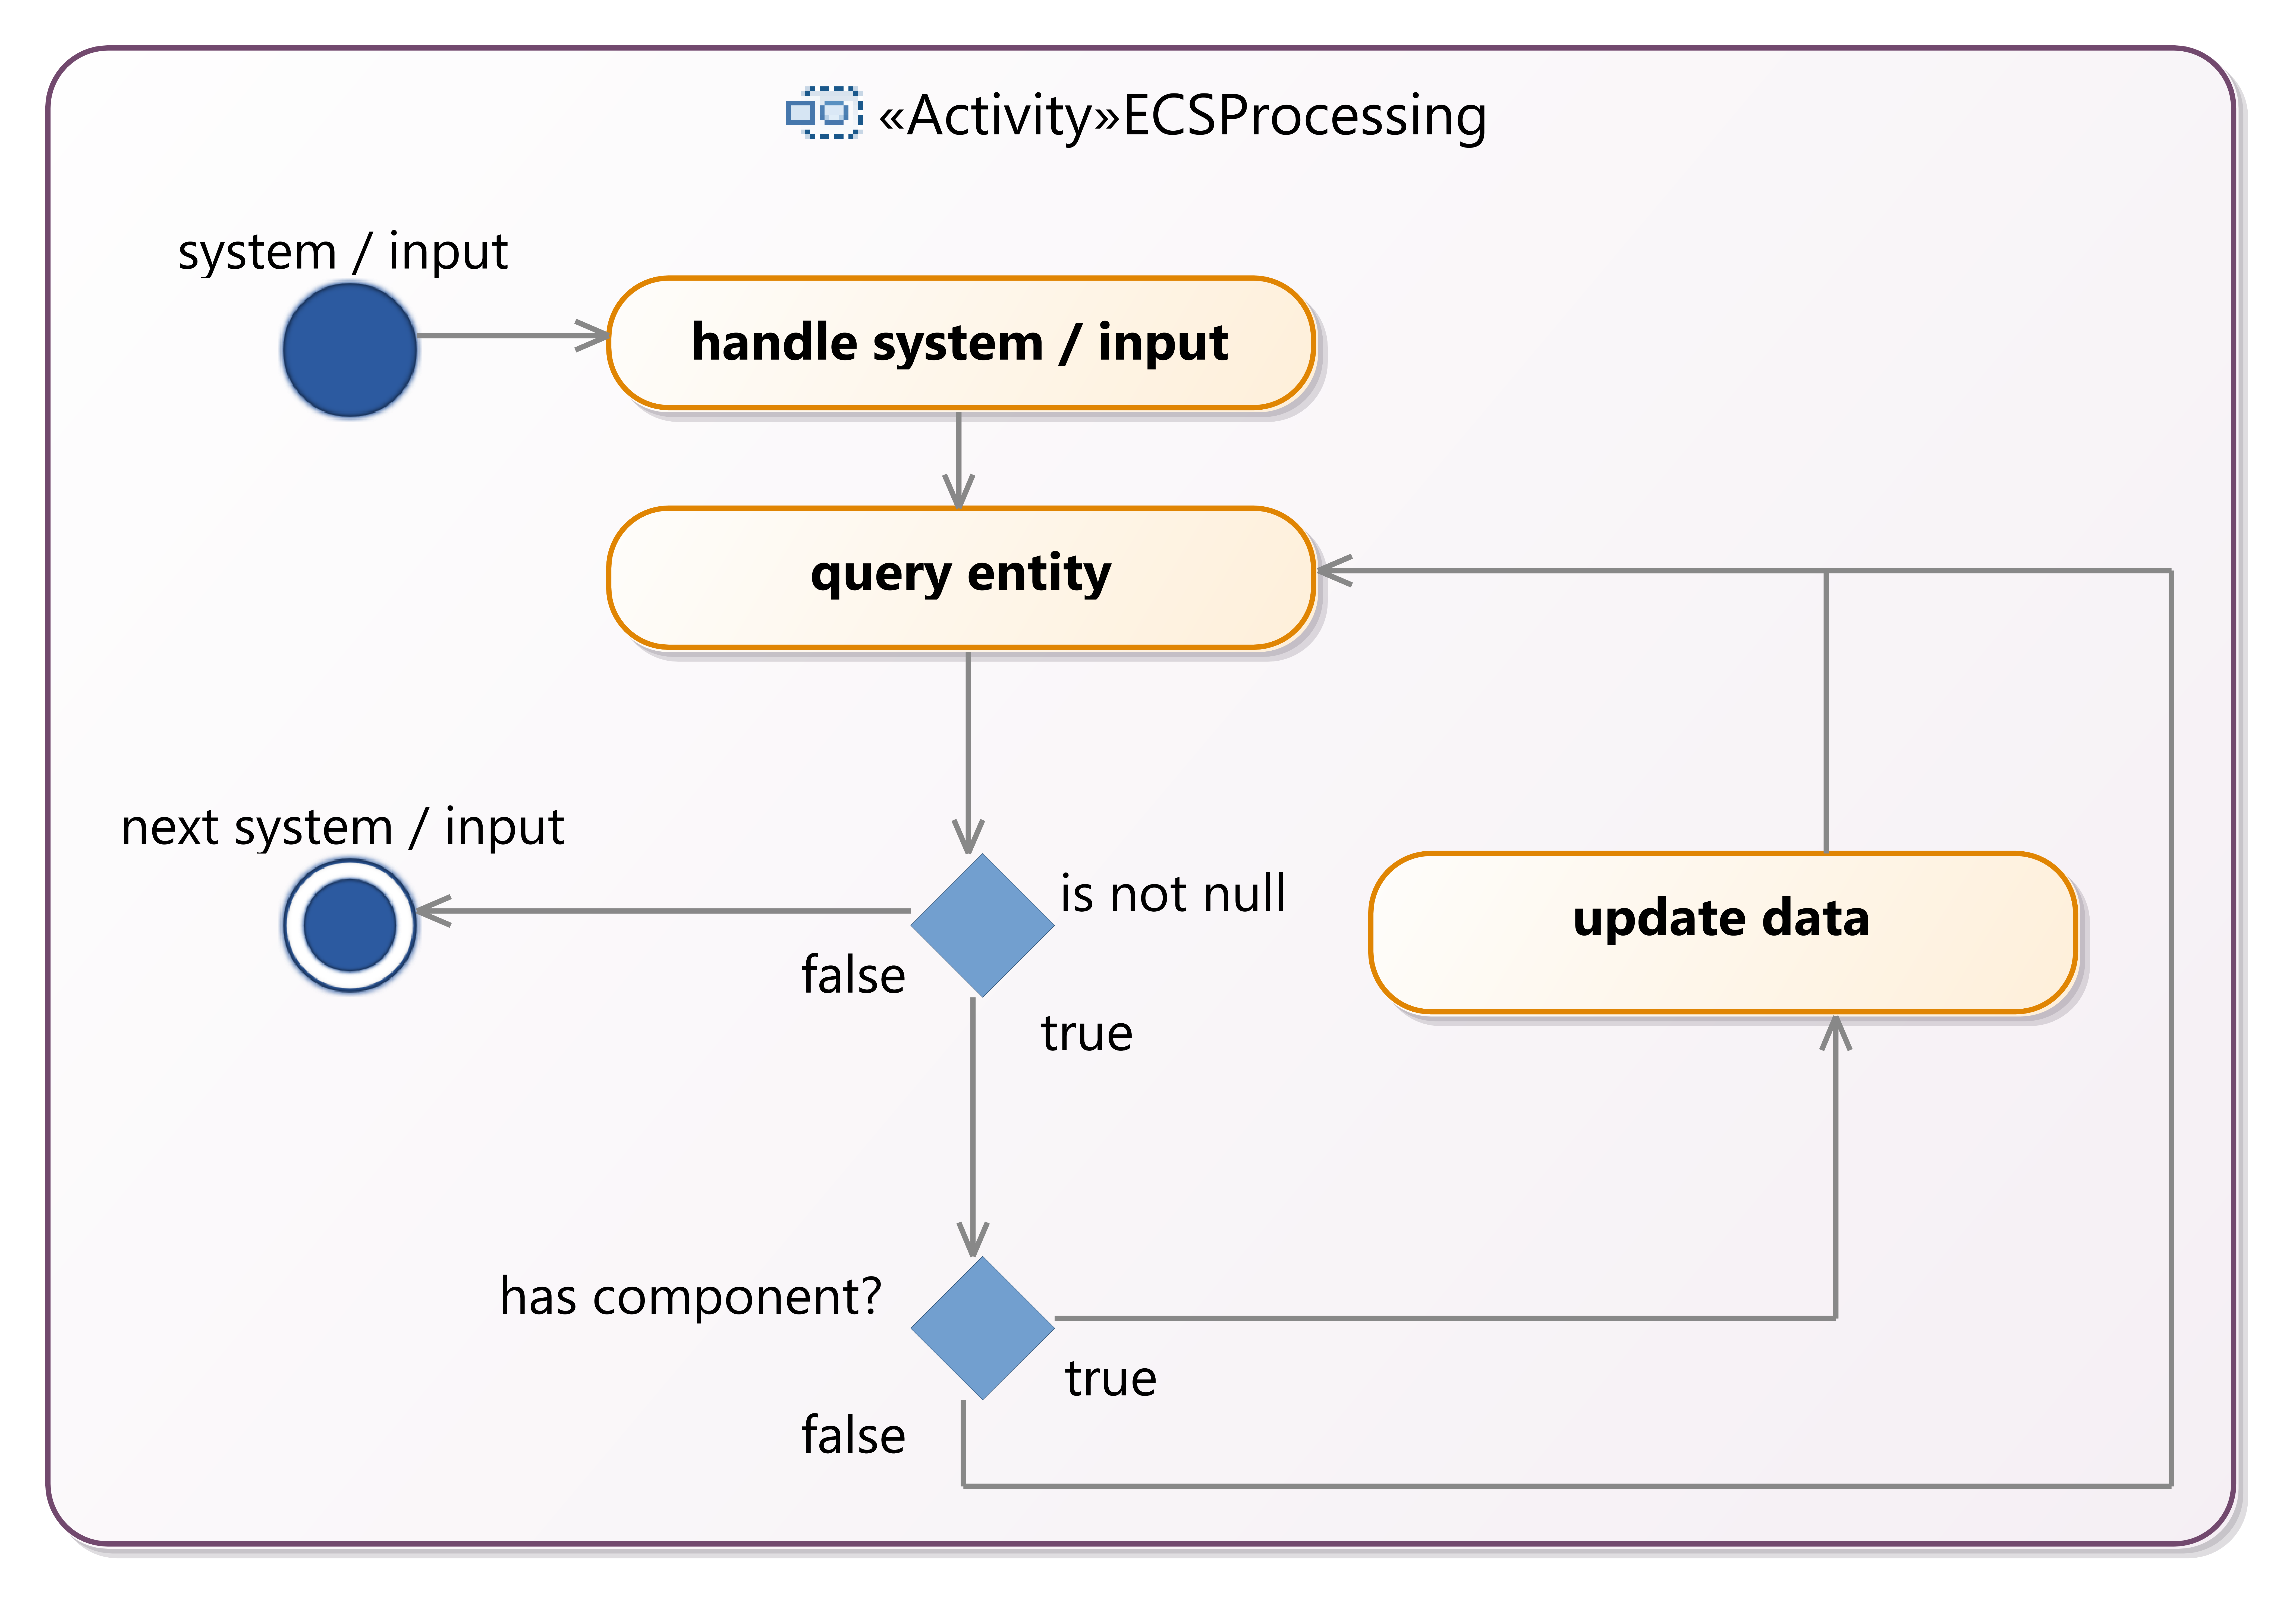
\includegraphics[width=\textwidth]{Pictures/res/implementation/ecs-system-processing}
    \caption{System processing activity diagram}
    \label{fig:ecs-system-processing}
\end{figure}
The systems implemented per default to this game engine are explained with reference to the \textit{GameLoop} implementation
as described in section~\ref{subsec:game-loop}.
\subsection{Game Loop}\label{subsec:game-loop}
The game loop acts as the main thread of the game as soon as initialized and started.
It packs all the different systems and handlers used in the game and executes them in a given order at every time step
$t_{i} = t_{i-1} + \Delta t$, where $\Delta t$ is the execution rate defined for the game.
An exception to this order is the input recording, which is handled in a separate, synchronized thread, as described in chapter~\ref{subsec:input-recording}.
In this implementation, $\Delta t$ is defined as $\Delta t = 1000 / 240 ms = 4.1667 ms$, which equals 240 calculated frames per second that may be shown and rendered
to the screen, if available.
\\ \\
The execution order of the game loop can be seen in figure~\ref{fig:gameloop-process}.
\begin{figure}
    \centering
    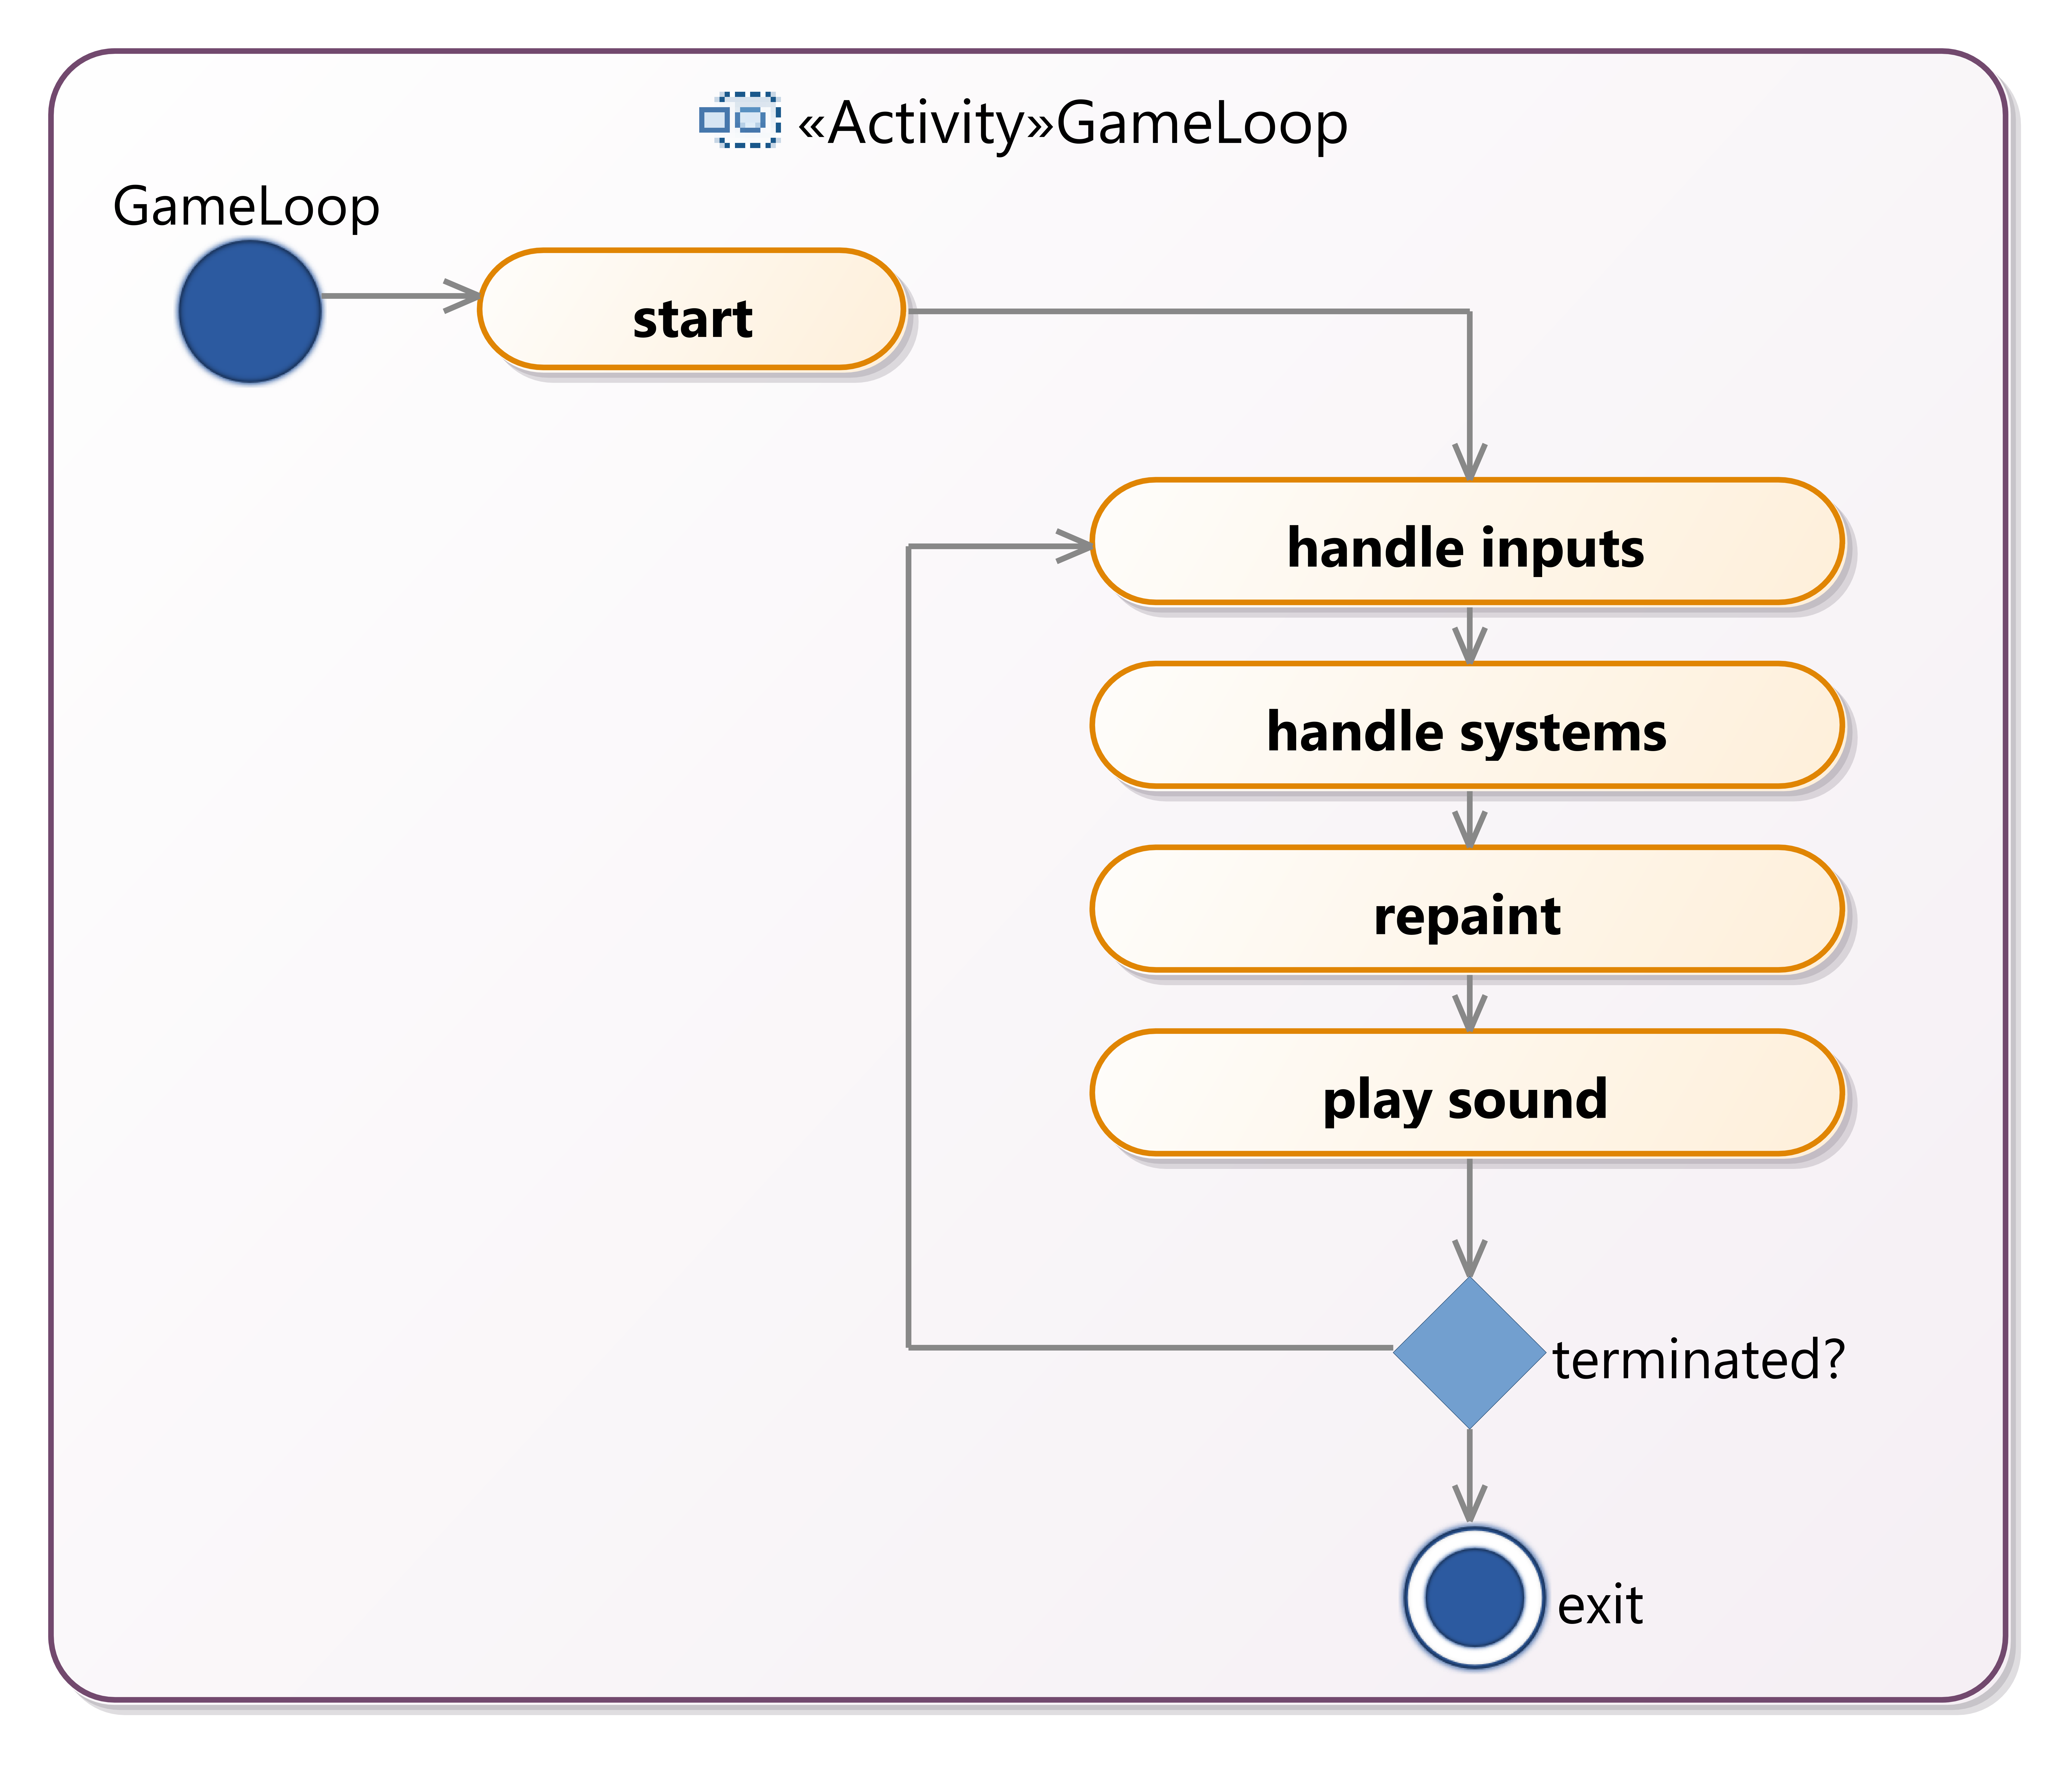
\includegraphics[width=\textwidth]{Pictures/res/implementation/gameloop-process}
    \caption{Game loop execution order}
    \label{fig:gameloop-process}
\end{figure}

\subsection{Input Recording}\label{subsec:input-recording}
Input recording is executed in a separate thread and handles inputs at a rate of $\Delta t_{inputs} = 20 ms$, since inputs in between two frames
would otherwise not be received by the games' input handling system.
$20 ms$ is a delta time that was found to be working best with the given circumstances.
It records all user inputs correctly while preventing unused overhead from recording more events than usable by the game systems.
\\
Generally, a button press needs to be differentiated from a button click.
While a button press is a continuous event, a button click is a one time event defined as the state change from button is not pressed to button is pressed.
Each recorded event, either from \textit{ActionListeners} implemented directly on the \textit{RenderingPanel} or from
the \textit{GamePadAdapter} are queued to the engines \textit{InputManager} as explained in section~\ref{subsec:input-handling}.
\\
The game pad integration is explained in section~\ref{subsec:gamepad-integration}, as this section mainly focuses on the recording of inputs itself.
\subsection{Input Handling}\label{subsec:input-handling}
The \textit{InputManager} contains a list of all \textit{Handlers} available to the game, implements methods to add and remove objects
of the \textit{Handler} class and methods to queue events
to a list of events per type - \textit{MouseEvent}, \textit{KeyEvent} and \textit{InputAction} (controller inputs).
\\
Each \textit{Handler} connected to the \textit{InputManager} receives all the events available in the respective event
queues at the given time step and execute their handling methods, which
then execute the actual actions on the game and its entities.
The handler class is an abstract class that can be extended to implement a variety of handlers, depending on the game requirements.
One specific handler class, the \textit{CollisionDetectionHandler} is implemented by default and allows for an easy implementation of hovering and clicking entities with a ColliderComponent.
It compares the current mouse position (given in the latest mouse event) and handles a potential collision with an Entity.

\subsection{System Handling}\label{subsec:system-handling}
\textit{Systems} are time-based and triggered with every update loop of the game.
\textit{Systems} do not have specific handling methods for input types, they operate solely time-based and execute a pre-defined logic.
They contain methods for different calculations, game logic or time-based events and actions.
Similar to the \textit{Handler} class, the \textit{System} class is an abstract class that can be extended from to implemented system classes according to the game requirements.
The \textit{ActionSystem} is already implemented, which is used to handle different types of actions that can be triggered e.g.\ by pressing a button entity, which starts
another scene.
The reason for this system being time based instead of event based is, that the \textit{CollisionDetectionHandler} already sets the state of the components,
however possible \textit{ActionComponents} need to be handled as well.
If a \textit{CollisionObject} is clicked or hovered, the \textit{ActionSystem} will check for possible actions to execute available from the \textit{ActionComponent}.

\subsection{Scene Update \& Repaint}\label{subsec:scene-update-&-repaint}
The next step in the game loop is a generic update of the currently active scene, which may be removing any unnecessary entities based on different conditions or
checking for a state change after an input or action has been handled.
After the update, the active scene is repainted by the \textit{RenderingEngine}~\ref{subsec:graphics-engine}.

\subsection{Rendering Engine}\label{subsec:graphics-engine}
The \textit{RenderingEngine} is a static class implemented within the game engine to handle all visible objects, screen rendering and scaling.
All content is rendered to a \textit{JPanel} object by using the \textit{Graphics2D} instance available by default, this is called the \textit{RenderingPanel}~\cite{jpanel,graphics2d}.
\\
The \textit{RenderingEngine} receives scaling factors for width and length from the \textit{ScalingEngine} and the \textit{RenderConfiguration}
classes, which handle resizing the frame,
fullscreen mode and different screen resolutions as well as antialiasing options.
During the rendering cycle, every location and boundary of the \textit{RenderObjects} is scaled and only afterwards it is rendered, however the original design position
is always present in the \textit{RenderObject} parameters.
This is necessary to correctly handle rescaling.
\\
A rendering cycle executes a few different methods which are all called by the overwritten repaint method from the \textit{RenderingPanel}.
First, all entities with a \textit{RenderComponent} are queried by the \textit{Query} system of the game engine and added to the rendering stack.
This stack is then split up into multiple stacks of \textit{RenderObjects}, which are the objects saved to the component that describe the actual
graphical visualization, based
on their rendering layer.
Each layer is rendered one after another by using specific rendering classes for different objects such as images, text or shapes.
Layering allows for stacking of multiple graphical entities above each other and allows for a better design and development flow GUIs and the game itself,
as the order of implementation and creation of entities is made obsolete through the usage of layers.
The following layers are rendered in this order:
\begin{enumerate}
    \item Background
    \item Game Layer 1
    \item Game Layer 2
    \item Game Layer 3
    \item Game Hover Layer
    \item UI Layer 1
    \item UI Layer 2
    \item UI Hover Layer
\end{enumerate}
For example, if a simple composition of background image, game entity and UI should be rendered at the same position,
the UI will always be in front of the game entity located at any of the game layers,
while the game entity will always overwrite the background at that position.
The reason for multiple UI and Game layers is simply to allow for a greater variety and range of possibilities when it comes to designing the game scenes.
\todo{add figure}.
\subsection{Sound Engine}\label{subsec:sound-engine}
A \textit{SoundEngine} is implemented in the game engine, which handles playing, pausing and stopping any audio stream available.
During each cycle, the \textit{SoundEngine} collects all entities with a \textit{SoundComponent} available, and checks if they are already playing and if not, if they should be playing.
The \textit{Java} built-in library \textit{Clip} is used to play audio streams and loop them if necessary~\cite{clip}.
This allows for an easy handling of any sound that should be played during a game, e.g.\ background music or button click sounds.

\subsection{Utility Classes}\label{subsec:utility-classes}
Detached from the \textit{GameLoop} execution, there are also multiple other configuration classes, managers, systems and utility classes, which will be briefly explained in this chapter.
\subsubsection{Game Configuration}\label{subsubsec:game-configuration}
The \textit{GameConfiguration} class by default implements a random profile name chosen of a variety of different names at game start, which is then used for saving high-scores
or may also be used in other parts of the game.
It also contains parameters for the currently active language, rendering configuration and sound configuration.

\subsubsection{Game Information}\label{subsubsec:game-information}
In the \textit{GameInformation} class, some generic variables for a title of the game, authors, version and description can be set, which are then used for instance as the games frame
title.

\subsubsection{Scene Manager}\label{subsubsec:scene-manager}
The \textit{SceneManager} is the main storage of all scenes, which may be menu scenes such as main menus or level scenes, i.e.\ game maps.
It can be called from anywhere within the game to switch a scene to another loaded scene or add a new scene to the scene stack.
Scenes should have unique identifiers (ids) in order for the \textit{SceneManager} to correctly load scenes from the stack.
\subsubsection{Resource Manager}\label{subsubsec:resource-manager}
The \textit{ResourceManager} is used for loading any kind of resource from outside the \textit{Java} classes, e.g.\ audio files, images or xml data and processes
these resources accordingly.
There are multiple implementations which are used by the \textit{ResourceManager} for loading of different XML files,
such as high-scores (\textit{HighScoreManager}) or languages (\textit{LanguageManager}),
however the basic implementation of the \textit{ResourceManager} equals their implementation and therefore the XML
parsing and processing is going to be described only for the \textit{ResourceManager}.
The following resource can be loaded by the resource manager and its sub manager classes:
\begin{itemize}
    \item Images, using the method \textit{loadImage()}
    \item Fonts, using the method \textit{loadFont()}
    \item Maps, using the method \textit{loadLevel()}
    \item Tilesets, using the method \textit{loadTileset()}
    \item Scores, using the method \textit{loadScores()}
\end{itemize}
\subsubsection{Logging}\label{subsubsec:logging}
The \textit{Java} logging tool is available and easily accessible from any class by simply using the static function
implemented in the \textit{Game} class and adding information to
the logger, which needs a specified log level and message to log.
Logging is and should always be implemented in stages of the game such as start, close or critical calculations, to identify possible bugs
easier.
\subsubsection{Styling \& Design}\label{subsubsec:styling-&-design}
A basic color scheme and font collection is already directly implemented to the game engine and may be used from scratch,
without loading other fonts or having to think about
color schemes.
This allows for a quick and easy design of graphical components.
\section{Game Implementation}\label{sec:game-implementation}
This chapter delves into the actual implementation of the game, highlighting the instances where the generic game engine is
employed and the reasons behind its use.
Additionally, it provides a comprehensive explanation of the various systems implemented to compute the game mechanics.
\subsection{Handler}\label{subsec:handler}
\textit{Handlers}, as already pointed out, are used to handle user inputs and trigger certain things within the game.
The implemented handlers for the game will be explained in this chapter.
\subsubsection{Build Handler}\label{subsubsec:build-handler}
The \textit{BuildHandler} is used to handle the placement, replacement, removal and connection of components to the game grid.
There are different \textit{SimulationTypes}, which are handled differently.
For the component and cable placement, the following constraints apply:
On each game grid tile, there may only be exactly one component of type \textit{ACTUATOR}, \textit{SENSOR}, \textit{COMPUTER} or \textit{VOTER}.
If any of the above-mentioned components exists on a tile, no cable may be placed at this position.
\textit{CABLE} type components are handled differently, as there may be cables of different types (red, blue, green, yellow) on the same tile, to enable
cross strapping of different components.
Cables can be rotated at both ends to correctly connect components as wanted.
Whenever a cable or component is placed or rotated, the connections are updated.
To display this connection, cable ports are used.
Each cable port can be used to connect a single other entity to the cable port.
Sensors have 4 cable ports with the type output, respectively actuators have 4 cable ports with type input.
Computers and voters have in and out puts, whereas cables only have a single in and output.
When replacing or removing a component, the removed component will be put back to the build panel and may be used again.

To summarize, the following features are currently implemented in the \textit{BuildHandler} class:
\begin{itemize}
    \item add items from inventory to grid
    \item remove items from grid
    \item replace items on the grid
    \item rotate cables (input and output)
    \item switching the cable layer currently used
\end{itemize}
\subsubsection{CursorSelectorHandler}\label{subsubsec:cursorselectorhandler}
For handling game pad and keyboard inputs, the \textit{CursorSelectorHandler} was implemented.
It creates a globally available entity (meaning, it is available in every scene), which displays a virtual cursor that can be
moved around by using the keyboard arrows or the joysticks of a gamepad.
It handles all input actions coming from gamepads and key events coming from the keyboard, and converts them to their according mouse events,
if necessary and defined.
This way, all other handler implementations only need to handle mouse events, which are virtually queued from the cursor selector handler.

\subsection{System}\label{subsec:system}
\subsubsection{Simulation System}\label{subsubsec:simulation-system}
The \textit{SimulationSystem} handles updates of the current components on the game field, as well as starting the game goal
validation by using the \textit{MarkovProcessor}, as explained in section~\ref{subsubsec:example-markov-chains}.
\\
Each cycle of the \textit{SimulationSystem} executes four different methods.
At first, the group ids of each simulation entity are updated, as well their input ids.
This is needed in order for every entity to know to which other entities they are connected, which is necessary to correctly
update their states, both during the building mode and during the Markov simulation, where these connections are copied.
After updating the state, the graphical representation of each state is changed, depending on the actual state.
This shows, if an entity is correctly connected and working, or if it is currently not connected.
\\
The Markov chain computation is executed in a separate thread, which enables accurate rendering of animations during
the calculation, such as the aircraft's movement through the sky.
Once the Markov chain calculation is complete, all states that result in a system failure - taking into account the level goal and
requirements (minimum functional components, system failure probability, maximum out-of-control components) - are identified and
summed up to determine the system failure probability.
This probability is calculated separately for both out-of-control and passive failures.
\\
Subsequently, if the probabilities align with the level target and the validation is successful, the total score is calculated using the probabilities,
the remaining components in the build panel, and a base level score.
\\
Each level has a predetermined base score upon completion.
\begin{equation}
    s_{base} = 100
    \label{eq:base-score}
\end{equation}
The probabilities of the current state calculated are compared to the target requirement failure probability by comparing the number of exponentials of 10 to each other.
\begin{equation}
    s_{accuracy} = 10 \cdot \lvert \log_{10} p(state) - \log_{10} p(goal)\rvert
    \label{eq:accuracy-score}
\end{equation}
The component score is defined as the sum of all components that are still available to the player in the build panel (excluding cables).
\begin{equation}
    s_{component} = \sum_{i = 1}^{n_{components}} 10
    \label{eq:component-score}
\end{equation}
The total score is the sum of the three previously calculated scores.
\begin{equation}
    s_{total} = s_{base} + s_{accuracy} + s_{components}
    \label{eq:total-score}
\end{equation}
Each score is shown separately in the score overview, with an additional indication of the accuracy of the probabilities to the target.
The user can see, where he or she may improve the system in order to get closer to the target.
This scale is also shown, when the validation of the target requirements is not passed by the currently built system, to indicate
a hint on what could be improved by the user.
\\
To correctly validate the goal, the actual probability calculated is summed up with an epsilon value of $\epsilon = 1e-7$,
to prevent incorrect validations due to rounding errors in double values.
The double precision floating point error occurs due to the internal representation, which can only represent a specified range of
values~\cite{floating-point}.
Therefore, especially when working with very small or very large numbers, rounding errors (i.e.\ the next representable value by the internal structure which can be stored
in the binary format) occur.
\subsubsection{Markov Processor}\label{subsubsec:example-markov-chains}
In this chapter, some examples for Markov chains that represent the level designs will be shown and the implementation of the
\textit{MarkovProcessor} will be explained by using these graphs.
\\ \\
The \textit{MarkovProcessor} generates a markov chain, based on the given entities and available groups and inputs provided by the \textit{SimulationSystem}.
First, a starting state, including all the relevant \textit{Entities} is generated.
Each state is represented as a \textit{MarkovState}, which contains the probability of the state occurrence, equalling the
transition rate, and a list of \textit{MarkovStateObjects},
that represent the different entities available after validating
the current level.
This step is needed in order to generate all the different \textit{MarkovStates} without actually modifying the game grid.
\\ \\
For demonstration purpose, a simple system state with a single sensor, computer and actuator is used.
Whenever a failure state is update to \textit{passive} or \textit{out-of-control}, all other components will also be updated accordingly,
which can also be seen in figure~\ref{fig:markov-simplex}.
The indices used are as follows: S = Sensor, C = Computer, A = Actuator.
The failure probabilities of each component is:
\begin{equation}
    \lambda_{f,S} = 1\text{e-}4
    \label{eq:markov-1}
\end{equation}
\begin{equation}
    \lambda_{f,C} = 1\text{e-}4
    \label{eq:markov-2}
\end{equation}
\begin{equation}
    \lambda_{f,A} = 0
    \label{eq:markov-3}
\end{equation}
For the failure detection ratio, the following values are used:
\begin{equation}
    C_{S} = 0.9
    \label{eq:markov-4}
\end{equation}
\begin{equation}
    C_{C} = 0.9
    \label{eq:markov-5}
\end{equation}
\begin{equation}
    C_{A} = 1
    \label{eq:markov-6}
\end{equation}

\begin{figure}
    \begin{center}
        \scalebox{0.33}{
            \begin{tikzpicture}[->, >=stealth', semithick, node distance=7cm, auto]
            \tikzset{rectangle/.append style={draw=black, thick, fill=white}}
            \node    (S)[font=\fontsize{24}{0}\selectfont]  {\TBox[fill=white]{Sensor}};
            \node    (C)[font=\fontsize{24}{0}\selectfont, right of=S]  {\TBox[fill=white]{Computer}};
            \node    (A)[font=\fontsize{24}{0}\selectfont, right of=C]  {\TBox[fill=white]{Actuator}};
            \path
    (S) edge (C)
    (C) edge (A)
            \end{tikzpicture}
        }
    \end{center}\caption{Example System System}
    \label{fig:simplex}
\end{figure}


\begin{figure}
\begin{center}
    \scalebox{0.33}{
        \begin{tikzpicture}[->, >=stealth', semithick, node distance=7cm, auto]
        \tikzset{rectangle/.append style={draw=black, thick, fill=white}}
        \node    (A)[font=\fontsize{20}{0}\selectfont]  {\TBox[fill=white]{C}\TBox[fill=white]{C}\TBox[fill=white]{C}};
        \node    (B)[font=\fontsize{20}{0}\selectfont,below of=A]   {\TBox[fill=white]{C}\TBox[fill=white]{F}\TBox[fill=white]{C}};
        \node       (C)[font=\fontsize{20}{0}\selectfont,left of=B] {\TBox[fill=white]{F}\TBox[fill=white]{C}\TBox[fill=white]{C}};
        \node (D)[font=\fontsize{20}{0}\selectfont,right of=B] {\TBox[fill=white]{C}\TBox[fill=white]{C}\TBox[fill=white]{F}};
        \node (G)[font=\fontsize{20}{0}\selectfont,below left of=B] {\TBox[fill=white]{C}\TBox[fill=blue!30]{P}\TBox[fill=blue!30]{P}};
        \node (H)[font=\fontsize{20}{0}\selectfont,below right of=B] {\TBox[fill=white]{C}\TBox[fill=red!30]{O}\TBox[fill=red!30]{O}};
        \node (F)[font=\fontsize{20}{0}\selectfont,left of=G] {\TBox[fill=red!30]{O}\TBox[fill=red!30]{O}\TBox[fill=red!30]{O}};
        \node (E)[font=\fontsize{20}{0}\selectfont,left of=F] {\TBox[fill=blue!30]{P}\TBox[fill=blue!30]{P}\TBox[fill=blue!30]{P}};
        \node (I)[font=\fontsize{20}{0}\selectfont,right of=H] {\TBox[fill=white]{C}\TBox[fill=white]{C}\TBox[fill=blue!30]{P}};
        \node (J)[font=\fontsize{20}{0}\selectfont,right of=I] {\TBox[fill=white]{C}\TBox[fill=white]{C}\TBox[fill=red!30]{P}};
        \path
    (A) edge[font=\fontsize{20}{0}\selectfont,left,pos=0.8]     node{$\dot{p_2}=\lambda_{f,C} \cdot p_1$}     (B)
        edge[font=\fontsize{20}{0}\selectfont,above left,pos=0.2]    node{$\dot{p_3}=\lambda_{f,S} \cdot p_1$}      (C)
        edge[font=\fontsize{20}{0}\selectfont,above right,pos=0.2]    node{$\dot{p_4}=\lambda_{f,A} \cdot p_1$}      (D)
        (C) edge[font=\fontsize{20}{0}\selectfont,above left,pos=0.5] node{$p_5=\dot{p_3} \cdot C_S$} (E)
        edge[font=\fontsize{20}{0}\selectfont,below right,pos=0.6] node{$p_6=\dot{p_3} \cdot (1-C_S)$} (F)
        (B) edge[font=\fontsize{20}{0}\selectfont,above left,pos=0.4] node{$p_7=\dot{p_2} \cdot C_C$} (G)
        edge[font=\fontsize{20}{0}\selectfont,above right,pos=0.4] node{$p_8=\dot{p_2} \cdot (1-C_C)$} (H)
        (D) edge[font=\fontsize{20}{0}\selectfont,below left,pos=0.8] node{$p_9=\dot{p_4} \cdot C_A$} (I)
        edge[font=\fontsize{20}{0}\selectfont,above right,pos=0.5] node{$p_{10}=\dot{p_4} \cdot (1-C_A)$} (J)
        \end{tikzpicture}
    }
\end{center}
\caption{Markov Chain Simplex System}
\label{fig:markov-simplex}

\end{figure}
The markov chain for these parameters can be seen in figure~\ref{fig:markov-simplex}.
\\
The implementation starts by generating a starting node, where all states are set to correct for the available components.
This state has a set probability of 1.
For each new state, the transition probability to this state from the previous state is calculated by multiplying the previous state probability with the
failure probability of the current failed component.
From there, each branch splits into two branches, one taking into consideration the failure detection ratio to calculate the passive failure state,
the other for calculating the out-of-control failure state.
\\
The approach of the implementation always sets the previous and the next states from a current state accordingly, so the tree-like
graph can be searched for specific states and state transitions.
Eventually, to receive the failure probability for a given state or a given set of states (e.g.\ all states that lead to a system failure), there is an algorithm
that finds exactly these states and calculates the sum of their probabilities.
Here, the failure probability for a time step of $t = 1 \text{h}$ is used, which results in a simplification of the general equations that removes all the integrations.
Therefore, only the state transition probabilities have to be summed up to calculate the actual probability for a specific set of states that can or cannot occur.
For larger or smaller time steps, instead of directly adding up the state transition probabilities, one would need to integrate the probability n times, based on the amount of nodes
/ states that are previous to each state.
\\
\\
A challenge during the implementation was the performance optimization for markov chains with increasing amount of system components.
There are two different approaches to the implementation, which are described below.
Additionally, an additional technique called ``Memoization'' is used to increase the performance even further.
\textbf{Recursive Markov Chain Generation}\\
New \textit{MarkovStates} are generated recursively, by calling the method from within the method directly after creating
and adding a new state to the next state list of a \textit{Markov State}.
This is calculated, until the break criteria is reached, which is, when a branch of the train is calculated until its very end,
where all \textit{MarkovStateObjects} are in
one of the two failed states, either OUT-OF-CONTROL or PASSIVE\@.
\textbf{Iterative Markov Chain Generation}\\
In the same way that states are calculated recursively, the same method was also implemented in an iterative manner,
after performance issues occurred with the recursion.
This is implemented via a stack, which is iterated through until it is empty.
With each iteration, new \textit{MarkovStates} are added to the stack, until each branch is finished, i.e.\ all \textit{MarkovStateObjects}
are in a failed state.
\textbf{Memoization}\\
To further optimize the algorithm, memoization was implemented.
Memoization is a programming technique used to optimize the execution time of computationally expensive functions by caching
their results for a given set of input parameters~\cite{10.5555/971738.971743}.
When a memoized function is called with the same input parameters as a previous call, the cached result is returned instead of re-computing the function.
In the implementation, a \textit{HashMap} is used, that stores each \textit{MarkovState} as a key-value pair by using a hash code
calculated from the current \textit{MarkovStateObjects} states.
Whenever another state change would require the \textit{MarkovProcessor} to calculate a state already available in this map, the \textit{MarkovState}
is instead cloned from there instead,
as the same \textit{MarkovState} means, that the exact same components have failed.

\subsection{Scene}\label{subsec:scenes}
A hierarchical scene structure was implemented to the game, which can be seen in figure~\ref{fig:scenes-hierachry}.
The base scene contains elements of the game that are visible in every scene, and therefore can be inherited to all other scene classes.
This includes the games background image and generic option buttons for settings, sound, back to menu and exit.
From this base scene, a base menu scene and a base game scene are inherited, which are used to display different menu screens and contain
the basic elements necessary to play the game or build maps in the build mode.
These scenes inherit multiple other scenes, which show different menus (main menu, level map, settings menu) and game scenes (main game scene, build mode scene, tutorial scene).
Specifically for tutorials, an interface which implements methods to display tutorial dialogues has been added to the game, which describes classes as tutorial classes.
Whenever a tutorial dialogue needs to be handled, this interface has to be implemented.

\begin{figure}
    \centering
    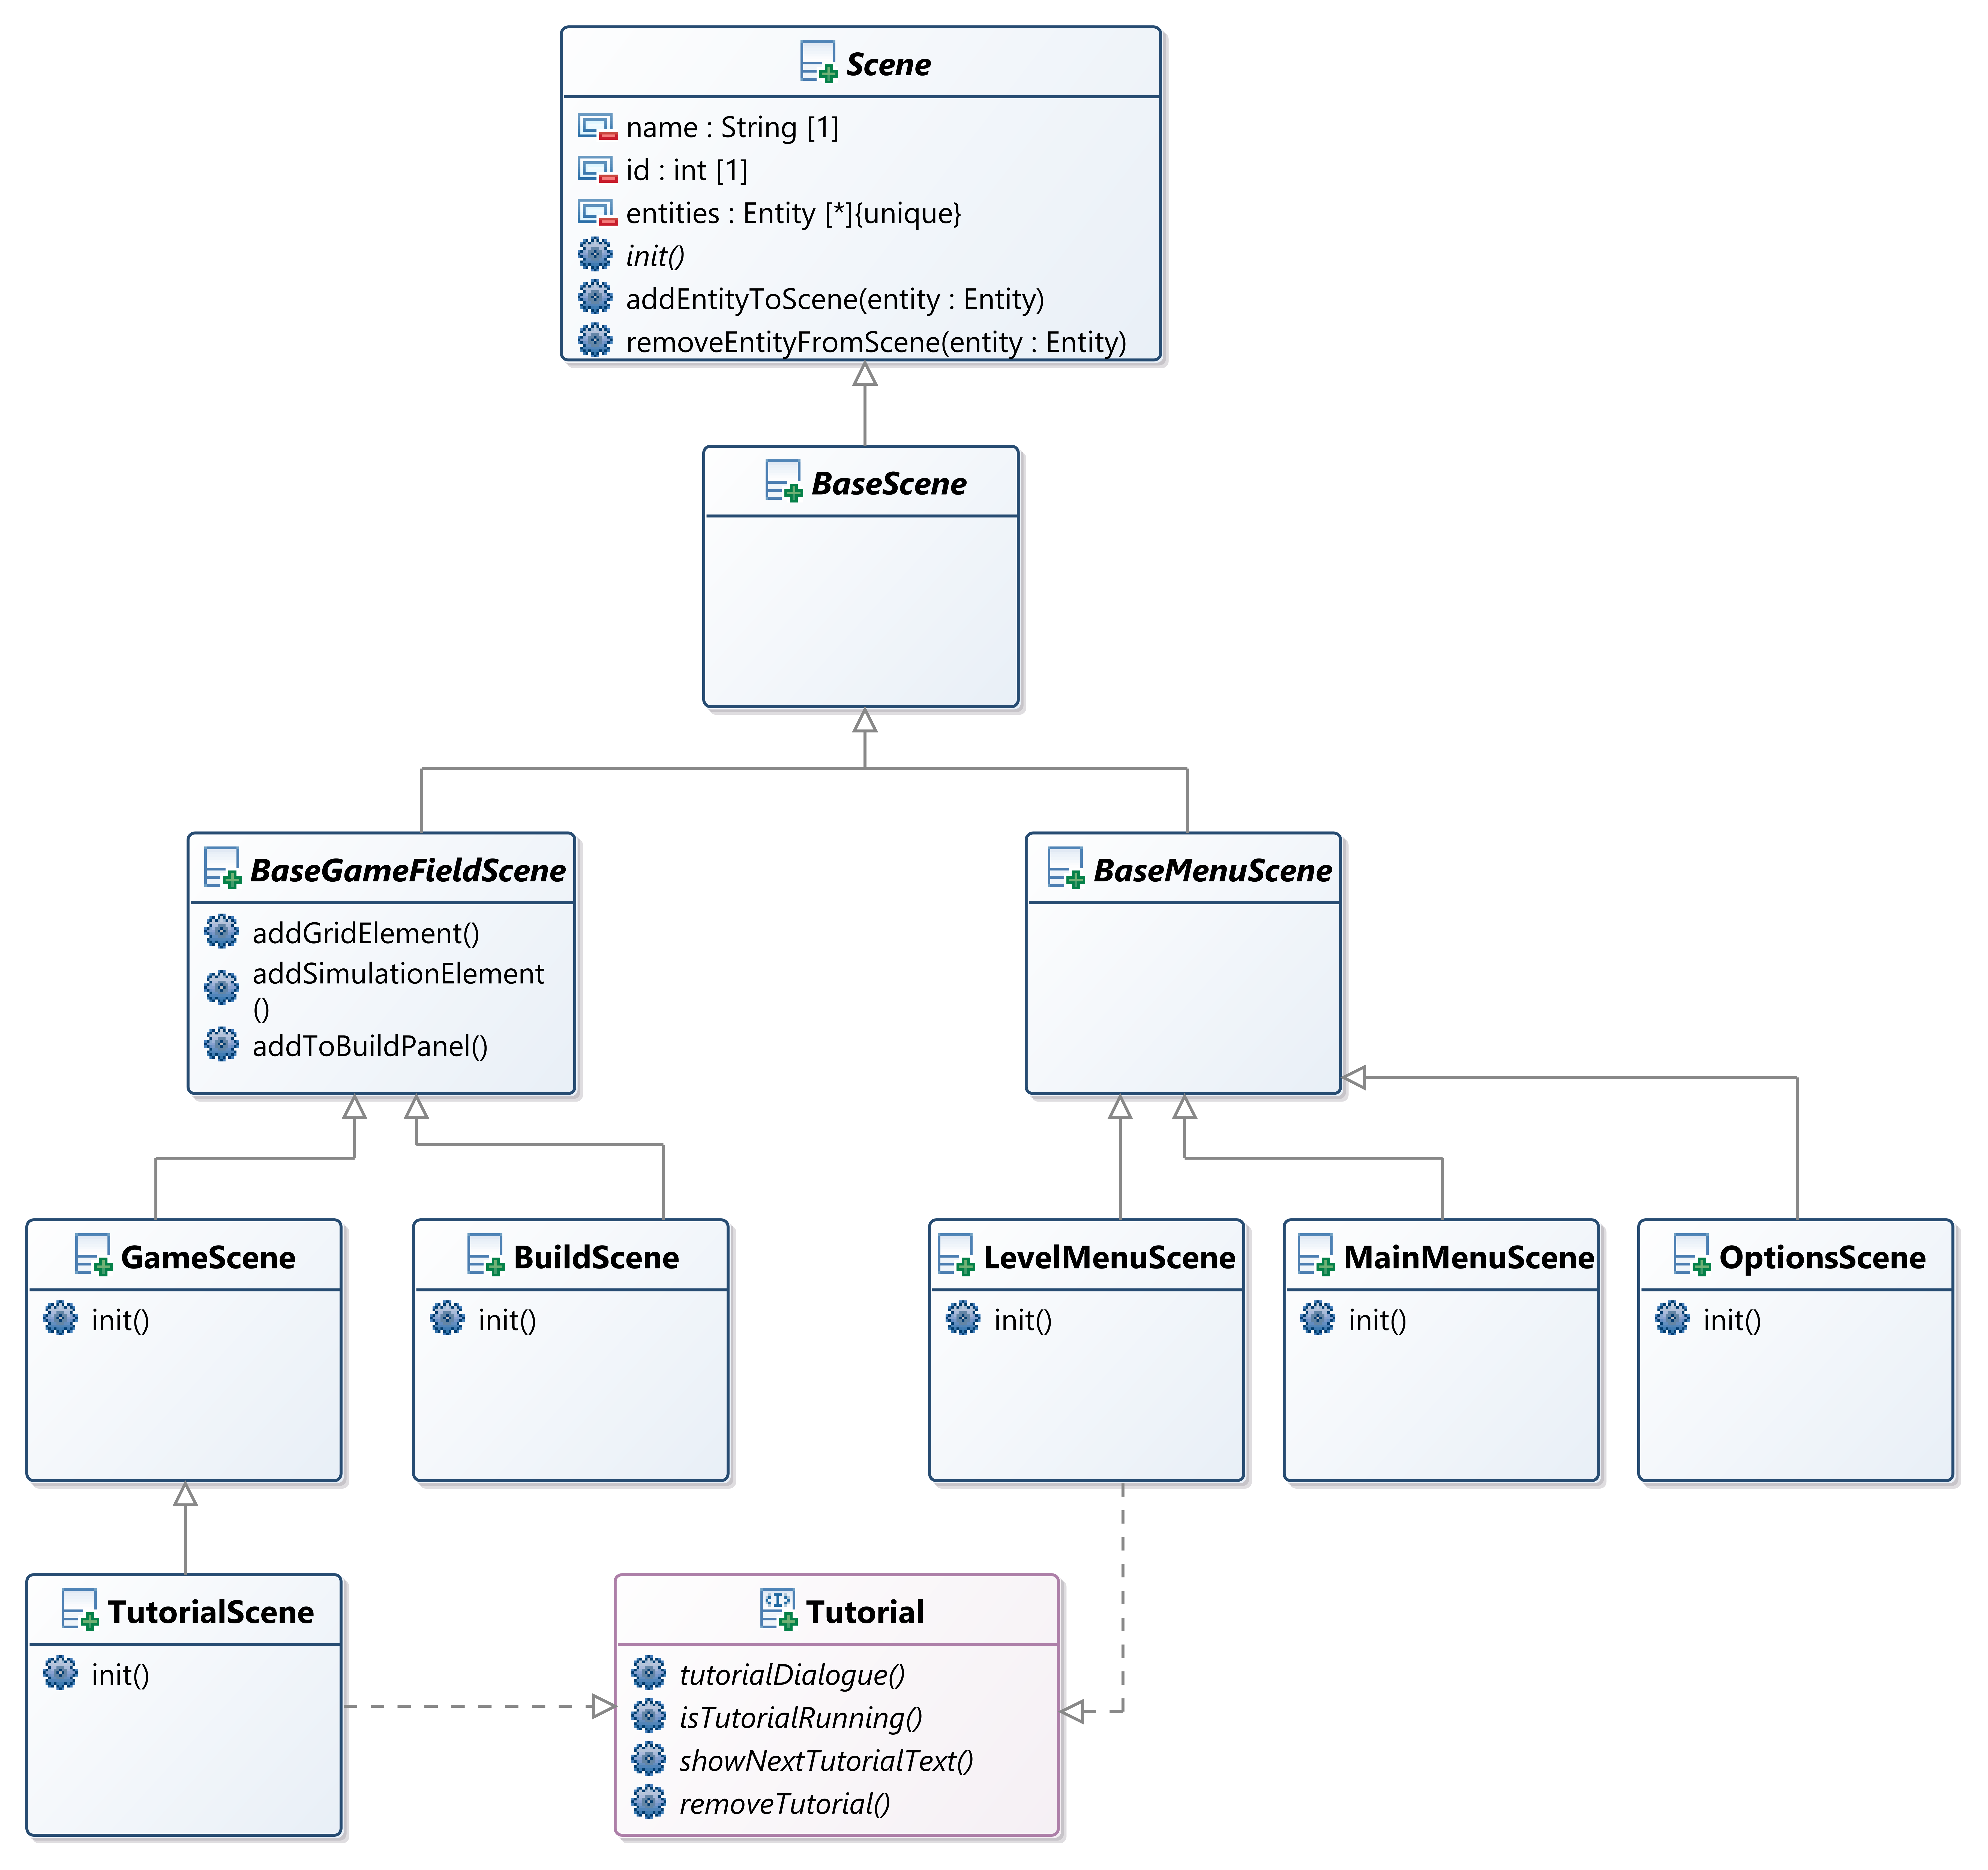
\includegraphics[width=\textwidth]{Pictures/res/implementation/scenes-hierarchy}
    \caption{Scene hierarchy}
    \label{fig:scenes-hierachry}
\end{figure}

The basic layout of the scenes was already described in~\ref{subsec:graphic-design}, the finished implementation of these
layouts is visualized in figures~\ref{fig:game-scene} and~\ref{fig:level-scene}.
Furthermore, the menu scene implementation is displayed in figure~\ref{fig:menu-scene}.

It is possible to create custom levels by using the build-mode, which is accessible through the build-mode scene, as shown in figure~\ref{fig:build-mode}.
The user can generate a grid of different sizes, set the amount of items that may be used from the inventory and place presets to
the grid that should be available on level start.
Furthermore, the goal requirements can be set via the save-button, where a name can be set.
The level is saved to a custom file, which may be loaded to the game manually.
\\
During scene design, a bright color palette was chosen to make the game environment appealing and playful.
For some elements, the color scheme of the Institute of Aircraft Systems was used (aircraft background, logo design).
The font used for the textual parts of the game is \textit{joystix monospace}~\cite{joystix}, which is a ``[\ldots] pixel-style
typeface inspired by 1980s arcade video games.
It's a timeless style that began with Atari in 1976 and extended to a slew of manufacturers throughout the 1980s.
It became the de facto font choice anytime a designer wanted to express classic videogame iconography in the twenty-first century''~\cite{joystix}.
As the main goal was to design an 8-bit styled, retro-like game, the font choice here is relatively obvious to make.
\begin{figure}
    \centering
        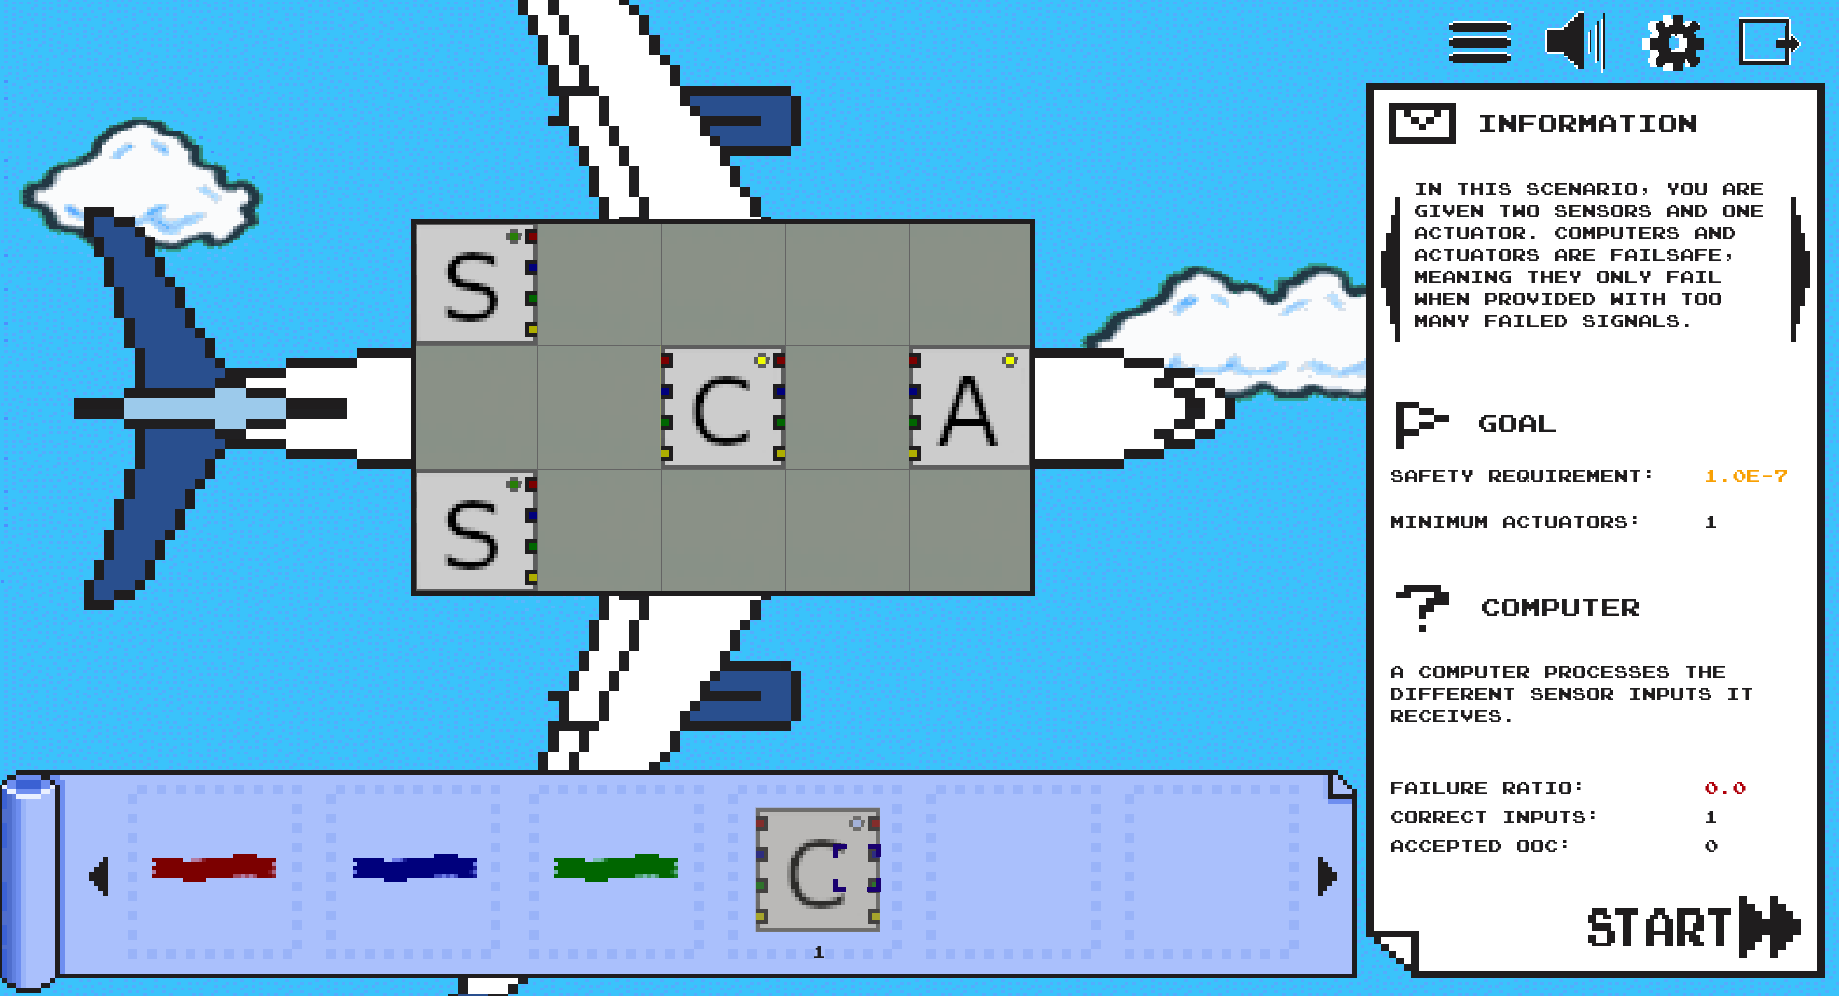
\includegraphics[width=0.9\textwidth]{Pictures/res/implementation/scenes/game-scene}
    \caption{Game Scene}
    \label{fig:game-scene}
\end{figure}

\begin{figure}
    \centering
        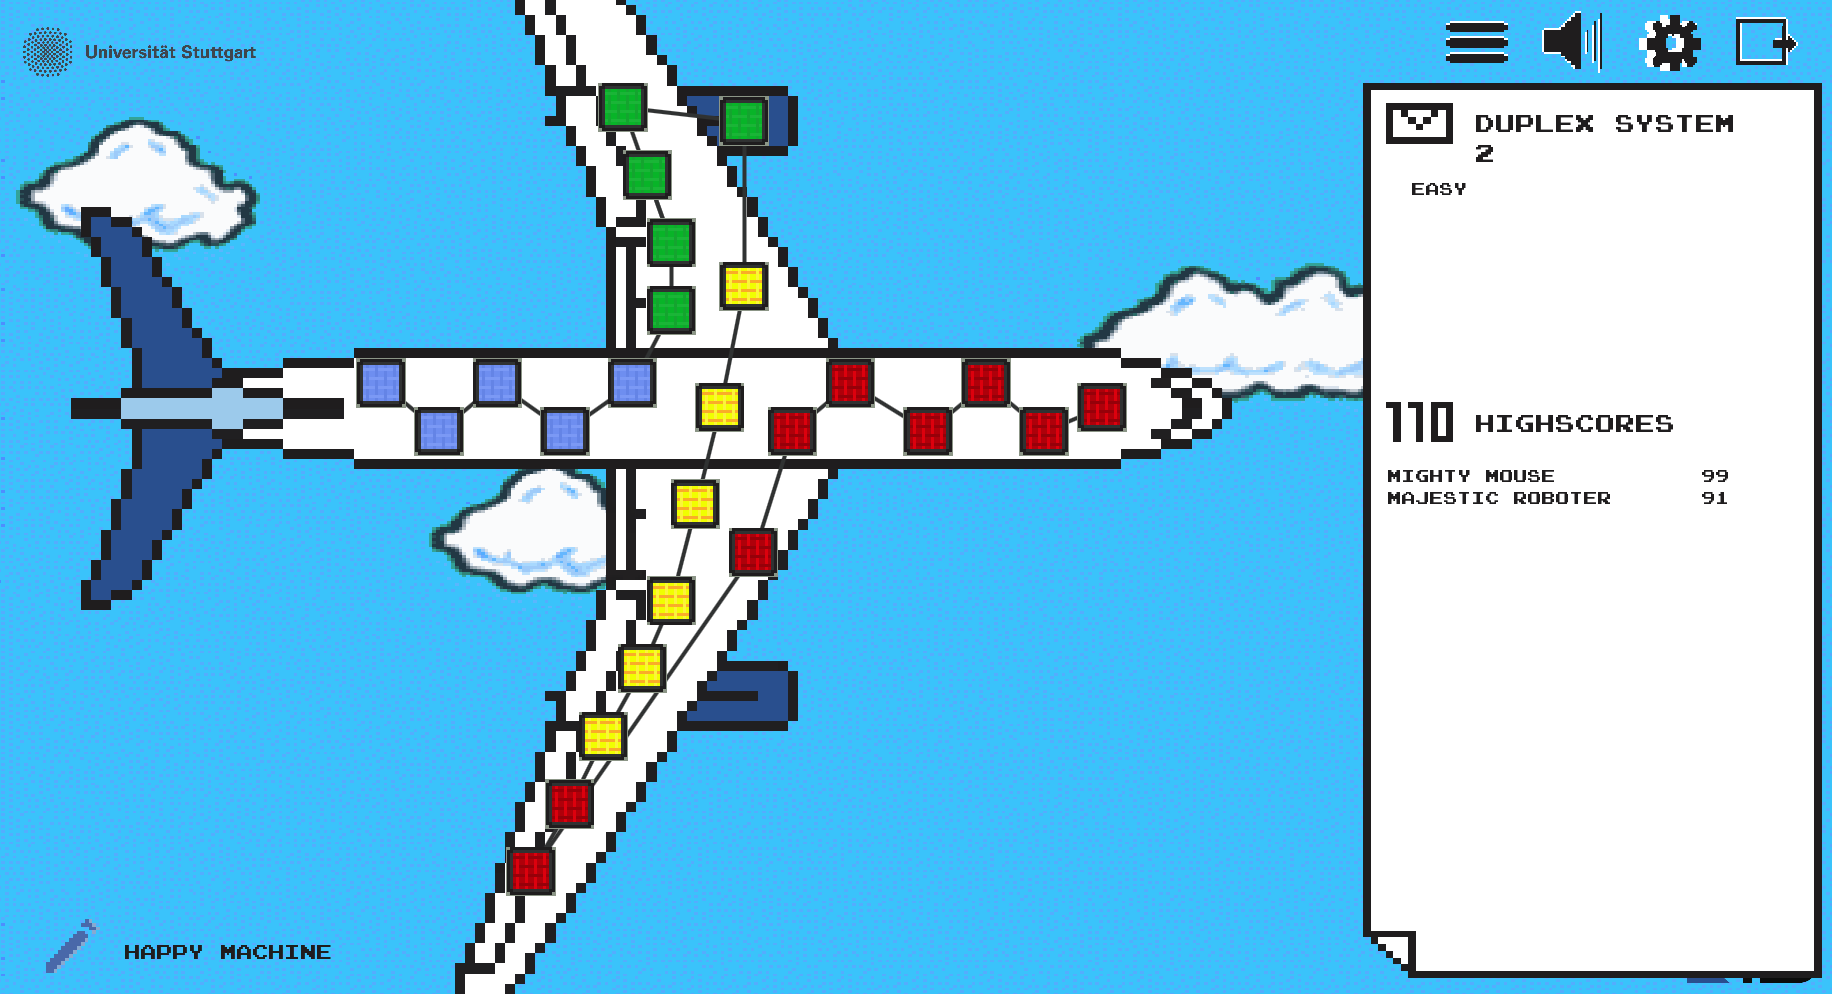
\includegraphics[width=0.9\textwidth]{Pictures/res/implementation/scenes/level-map}
    \caption{Level Map Scene}
    \label{fig:level-scene}
\end{figure}

\begin{figure}
    \centering
        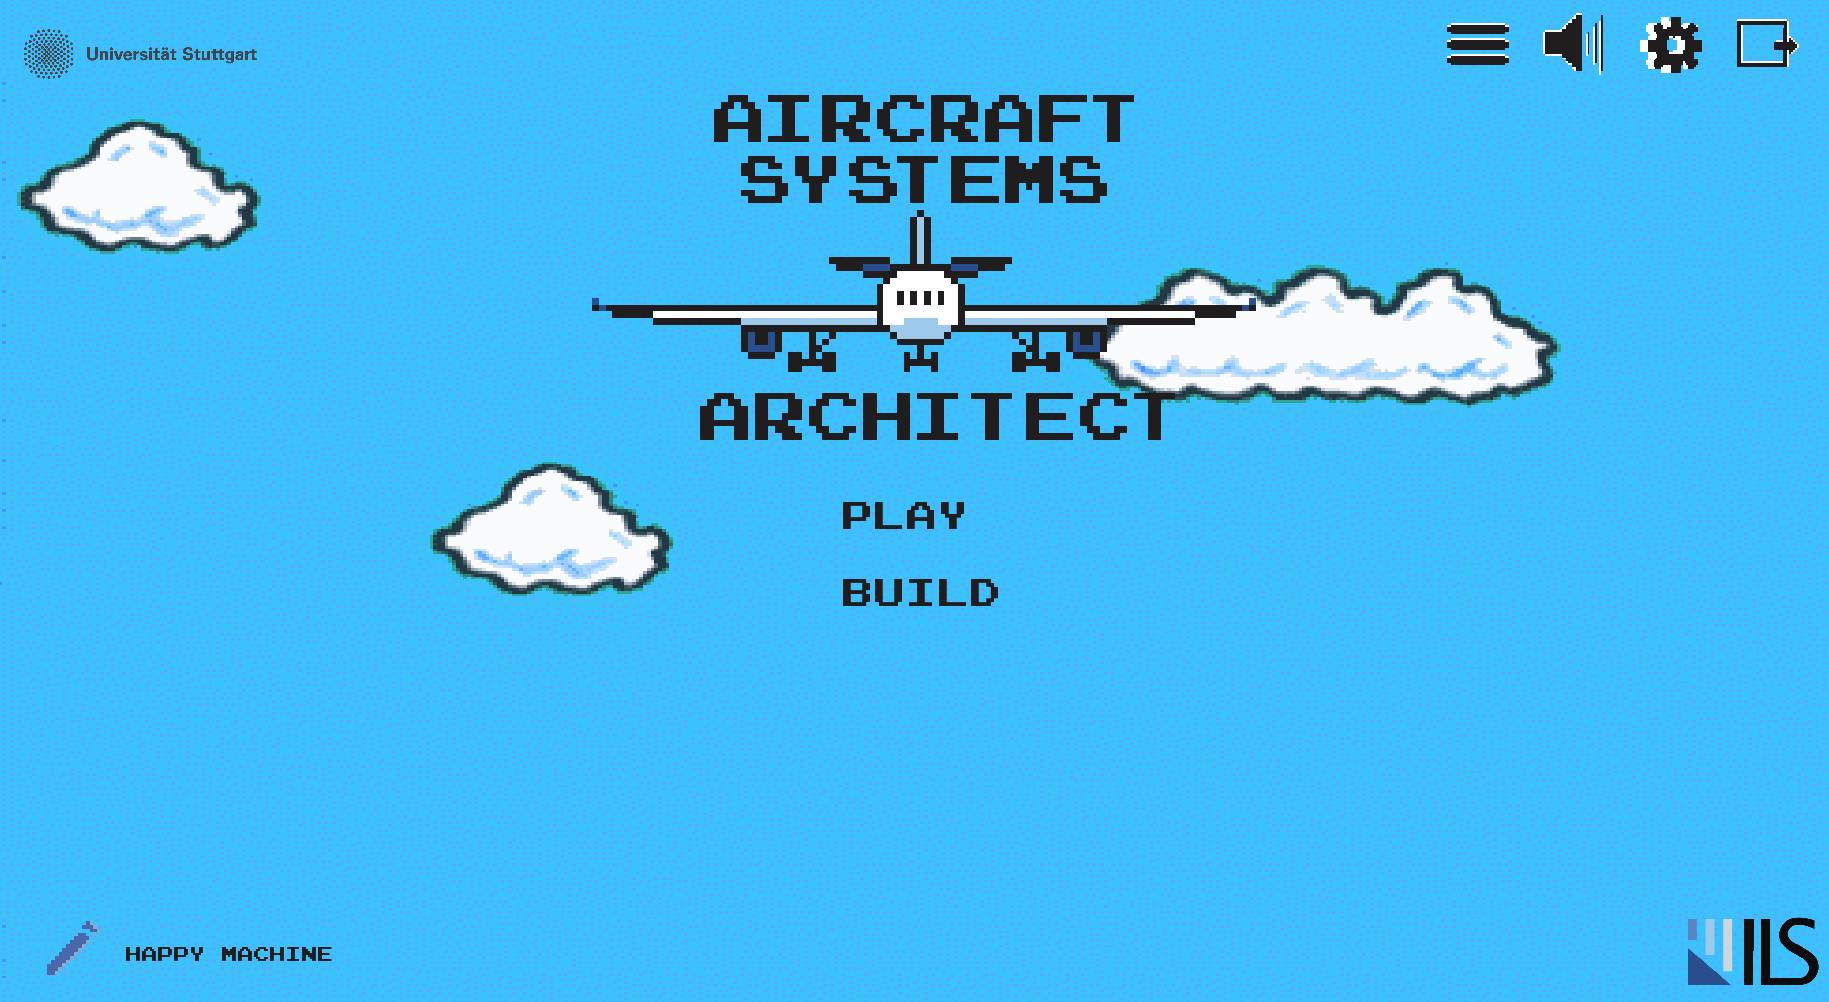
\includegraphics[width=0.9\textwidth]{Pictures/res/implementation/scenes/main-menu}
    \caption{Menu Scene}
    \label{fig:menu-scene}
\end{figure}

\subsubsection{Entities}\label{subsubsec:entities2}
The entities in the games' scenes are implemented as generified objects that can be instantiated.
The following entities are currently available in the game implementation.
\textbf{Grid Entities:} \\
\textit{GridEntities} describe each tile of the grid, containing a grid position as $(x,y)$ coordinates and a customizable grid tile,
which is usually the regular concrete background, but may be changed any time for specific scenarios.

\textbf{Simulation Entities:} \\
All elements that are placed on the game grid are considered so-called \textit{SimulationEntities}.
These entities are built of components to describe the cable port distribution, parameters such as failure ratio and failure detection ratio and grid components, which contain the
entities position as a coordinate in the games' grid-like game field.
Each entity that should have a description on the right side tool box also has a \textit{TooltipComponent} attached, which indicates, that
a tooltip should be shown when hovering the entity.
Furthermore, graphics and colliders are available to simulation entity objects.

\textbf{Build Panel Entities:} \\
\textit{BuildPanelEntities} are entities which are available in the players' inventory and can be used for building objects on the game grid.
They include components for graphics description, build information - e.g.\ the failure ratio, failure detection ratio and amount in inventory,
and colliders.
Similar to the \textit{SimulationEntity}, a tooltip component is also available to the build panel entities to indicate tooltip descriptions.
\subsubsection{Components}\label{subsubsec:components2}
The above-mentioned entities implement different components to store the according data and to identify which component
should implement certain behaviors such as being able to be built to the grid or adding them to the simulation.
The following components were developed and implemented during the game development process.

\textbf{GridComponent:} \\
The \textit{GridComponent} stores the grid position as $(x,y)$ coordinates of an entity, where $x=0, y=0$ is the top left of the game grid.

\textbf{SimulationComponent:} \\
Data regarding the simulation run by the \textit{MarkovProcessor} is stored in the \textit{SimulationComponent}.
The simulation type (i.e.\ Actuator, Sensor, Computer, \ldots), as well as the current state (i.e.\ inoperative, correct by default, \ldots), failure
ratio and failure detection ratio are stored.
Furthermore, the component contains parameters to store the entity ids of entities connected as inputs to this component / entity, which is
not necessary, however enables easier maintainable code and performant look-ups for some systems.

\textbf{BuildComponent:} \\
The \textit{BuildComponent} is used to tell the systems operating the game, that an entity should be buildable.
Therefore, it contains similar information as the simulation component, as the parameters from the build component are used
to create new \textit{SimulationEntities} with \textit{SimulationComponents} attached when placing a component on the grid.
Furthermore, the \textit{BuildComponent} also stores the amount of components on the stack.
As this number would go below 0, no new component can be built.

\textbf{CablePortsComponent:} \\
\textit{CablePortsComponents} contain data regarding the connection of entities to each other.
Each \textit{CablePortComponent} can have multiple in- or outgoing cable ports.
\textit{CablePorts} are used to store another entity object, which describes the entity connect to another entity.
When updating a connection, both sides of the connection have to be considered.
A cable ports' connected entity parameter may be null, when there is currently no connection to the port.

\textbf{TooltipComponent:} \\
The \textit{TooltipComponent} may be used for entities that should display a tooltip upon hovering over the object with the cursor.
Information such as failure ratio, simulation type and description of the object are stored as text strings (as ids, which are read
from the language file, or as converted numbers to strings) in this component, so they may be directly used to render them to
the screen.
\subsubsection{Entity UML}\label{subsubsec:entity-uml}
A comprehensive overview of the different entity structures is given in figure~\ref{fig:entities}.
\begin{figure}
    \centering
    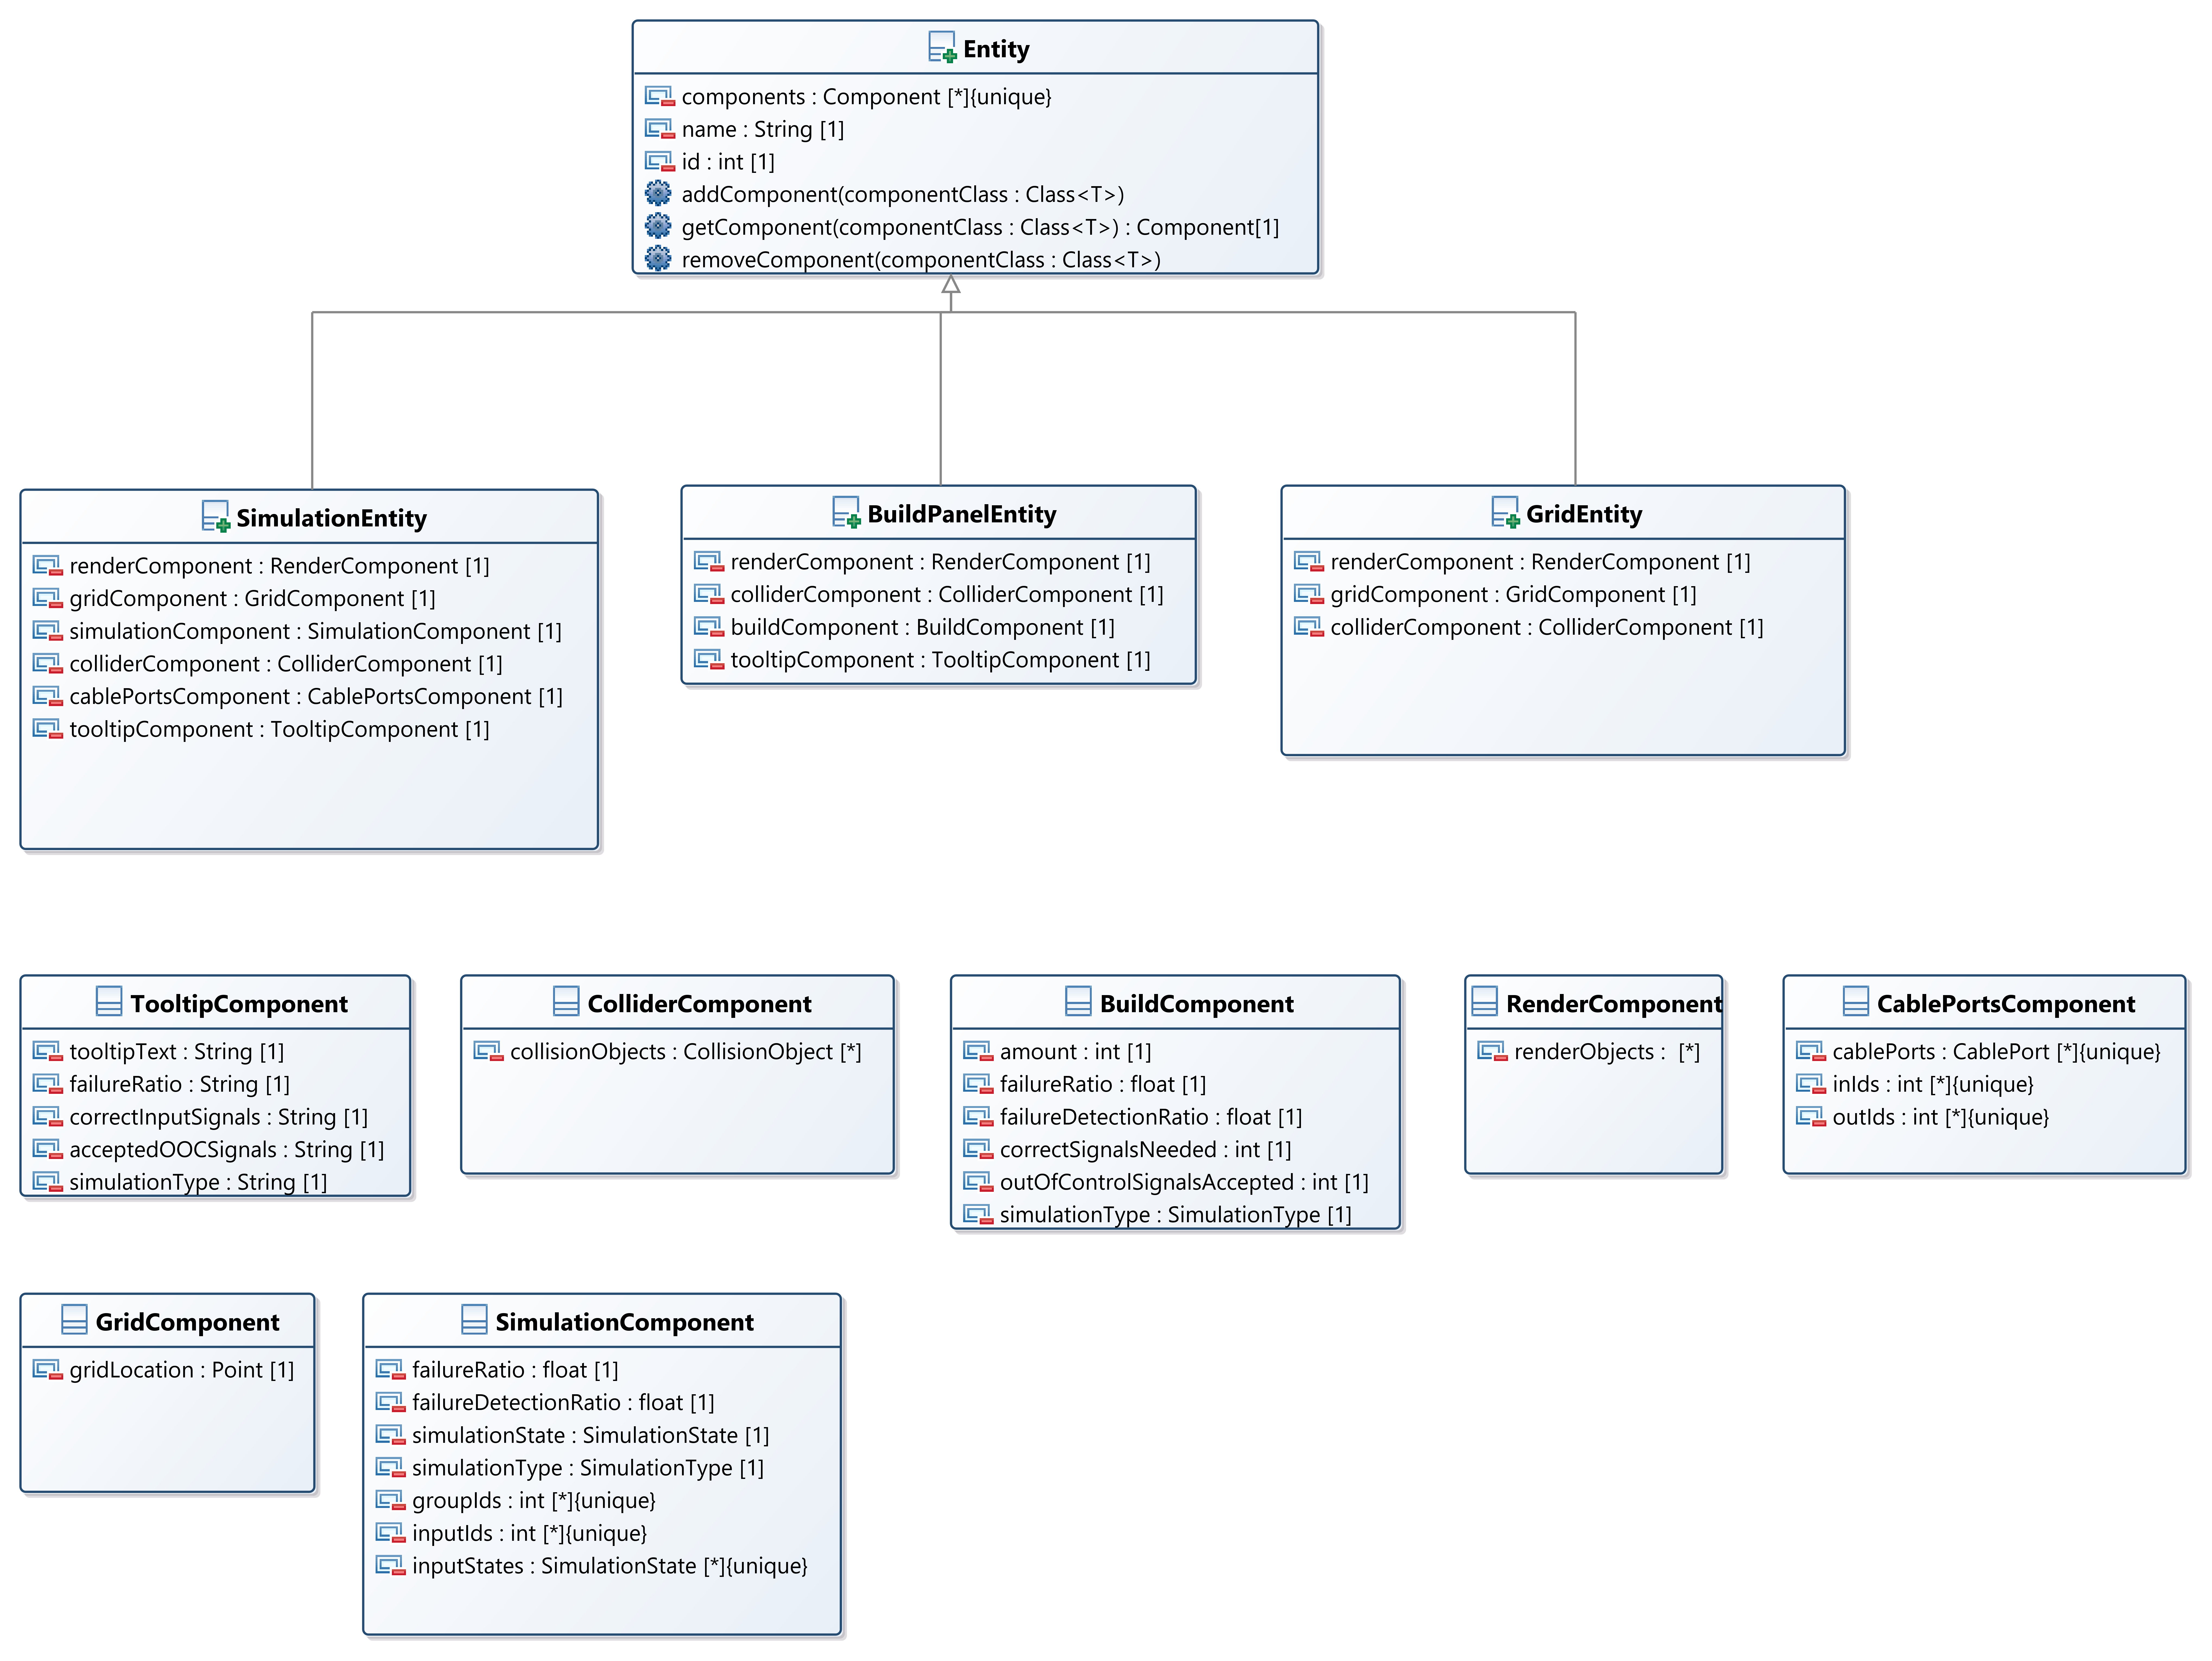
\includegraphics[width=\textwidth]{Pictures/res/implementation/entities}
    \caption{UML Diagrams of the different entities}
    \label{fig:entities}
\end{figure}
\subsection{Level Implementation}\label{subsec:level-implementation}
Each level is created as a new \textit{GameScene} object with the content of a level file that is read and parsed by the \textit{ResourceManager}
~\ref{sec:data-storage-&-data-parsing}.
The \textit{GameScene} object stores all relevant data, including the level requirements / goal, the grid size, available entities and,
if applicable through the
tutorial interface implementation, possible dialogues and character models that form the tutorial scene.
Following examples for different levels are provided in this chapter:
\begin{itemize}
    \item Tutorial Scene explaining the basics of the gameplay~\ref{fig:basic-gameplay-tutorial}
    \item Duplex System~\ref{fig:duplex-system}
    \item Common-Mode Scenario, with different types of sensors and computers~\ref{fig:common-mode-scene}
    \item Oil leakage scenario, emulating a common-cause failures~\ref{fig:common-cause-scene}
\end{itemize}
\todo{add scene pictures}
\begin{figure}
    \centering
    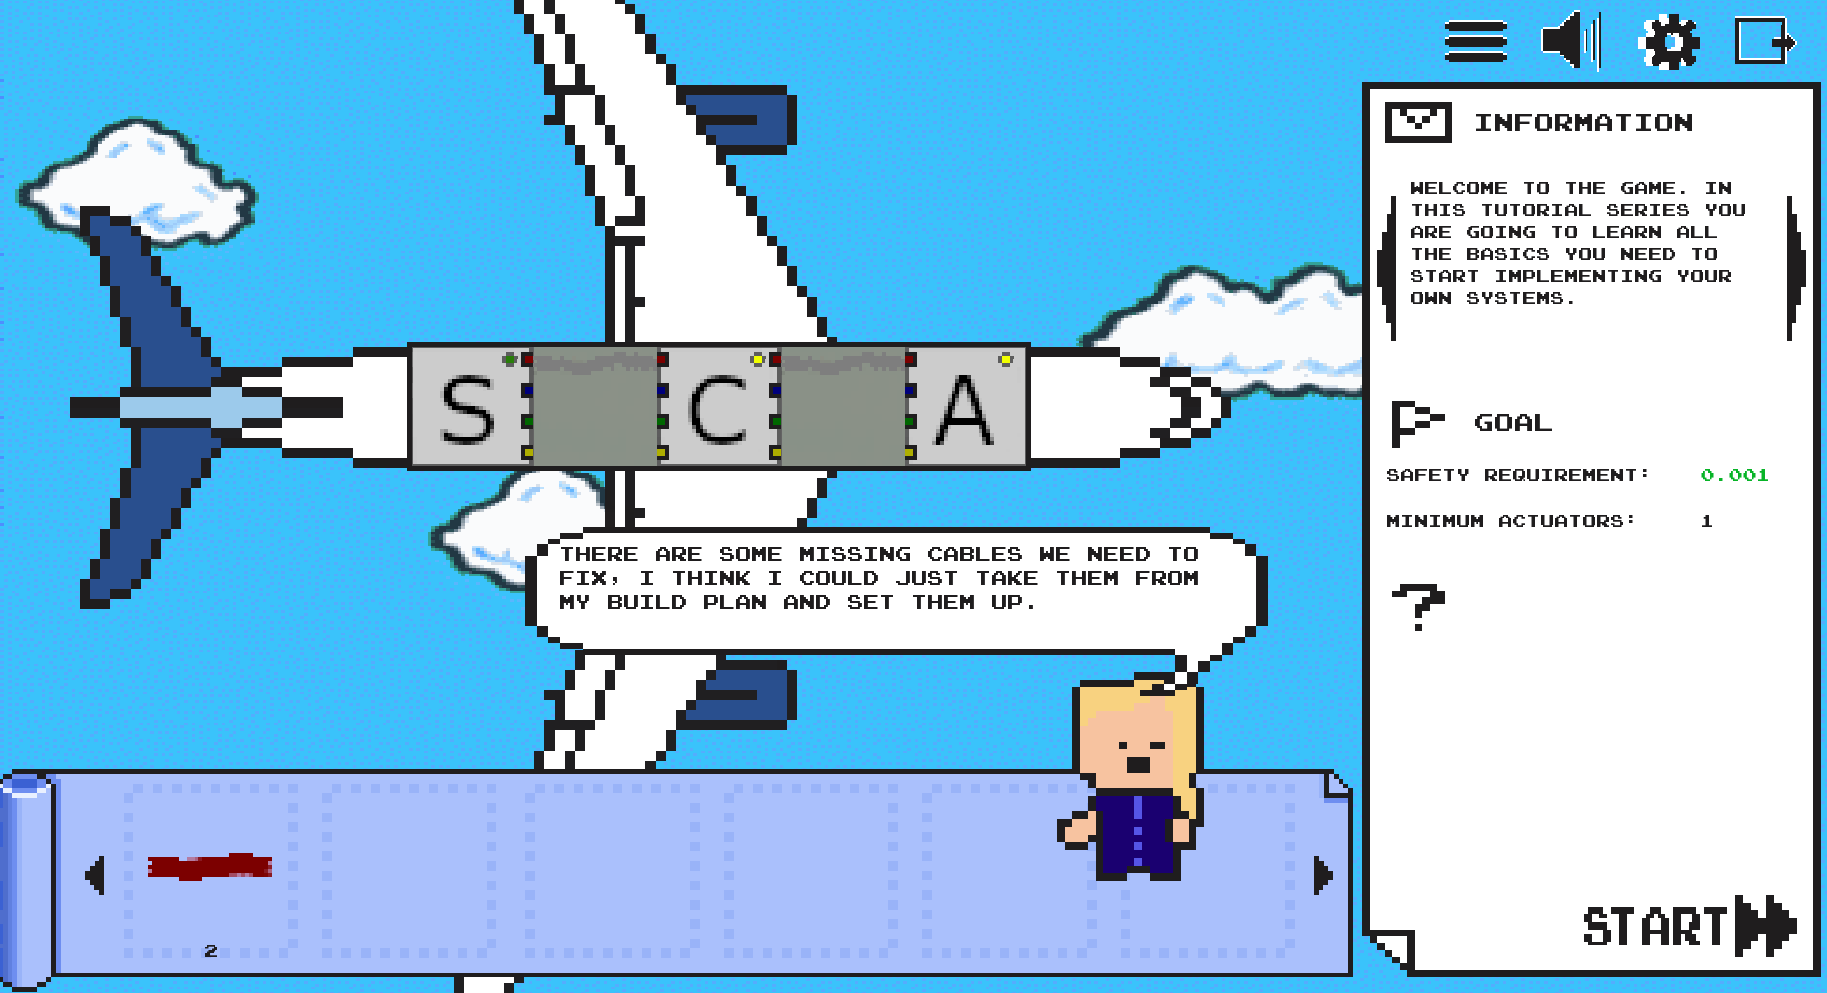
\includegraphics[width=\textwidth]{Pictures/res/implementation/scenes/tutorial-game-scene}
    \caption{Tutorial Scene with dialogue to explain basic gameplay}
    \label{fig:basic-gameplay-tutorial}
\end{figure}
\begin{figure}
    \centering
    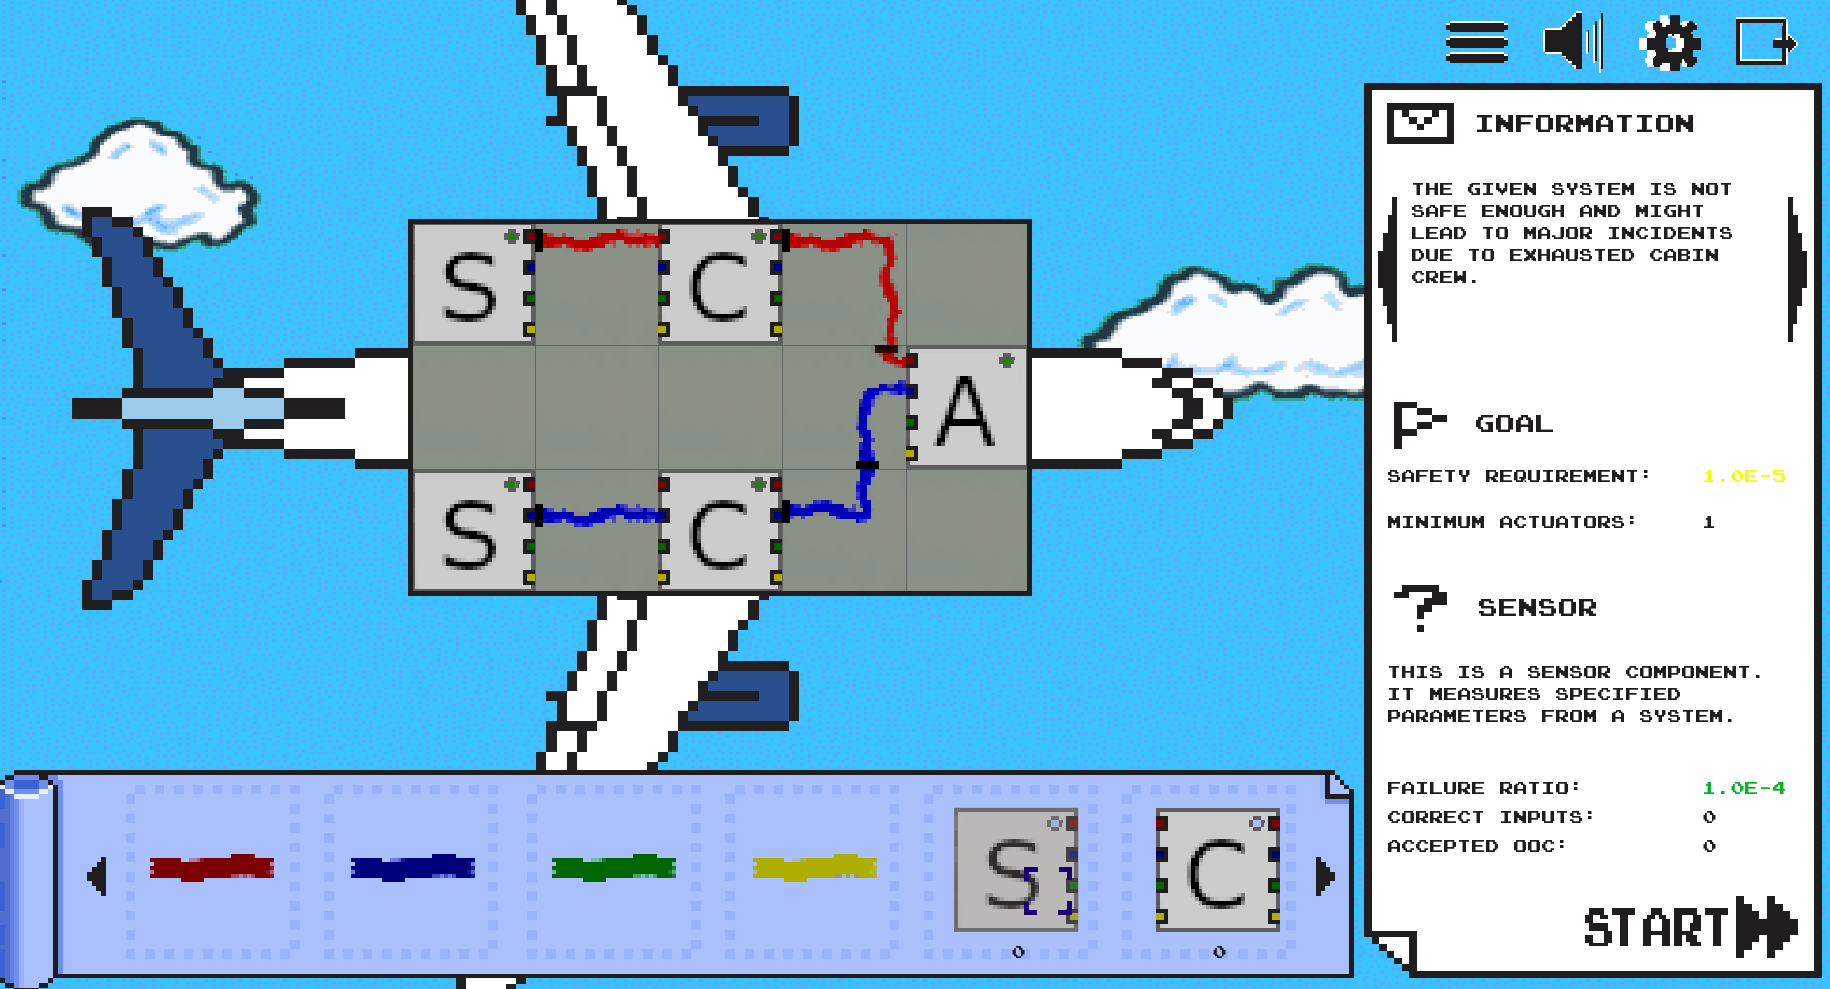
\includegraphics[width=\textwidth]{Pictures/res/implementation/scenes/duplex-scene}
    \caption{Scenario to set up a duplex system}
    \label{fig:duplex-system}
\end{figure}
\begin{figure}
    \centering
    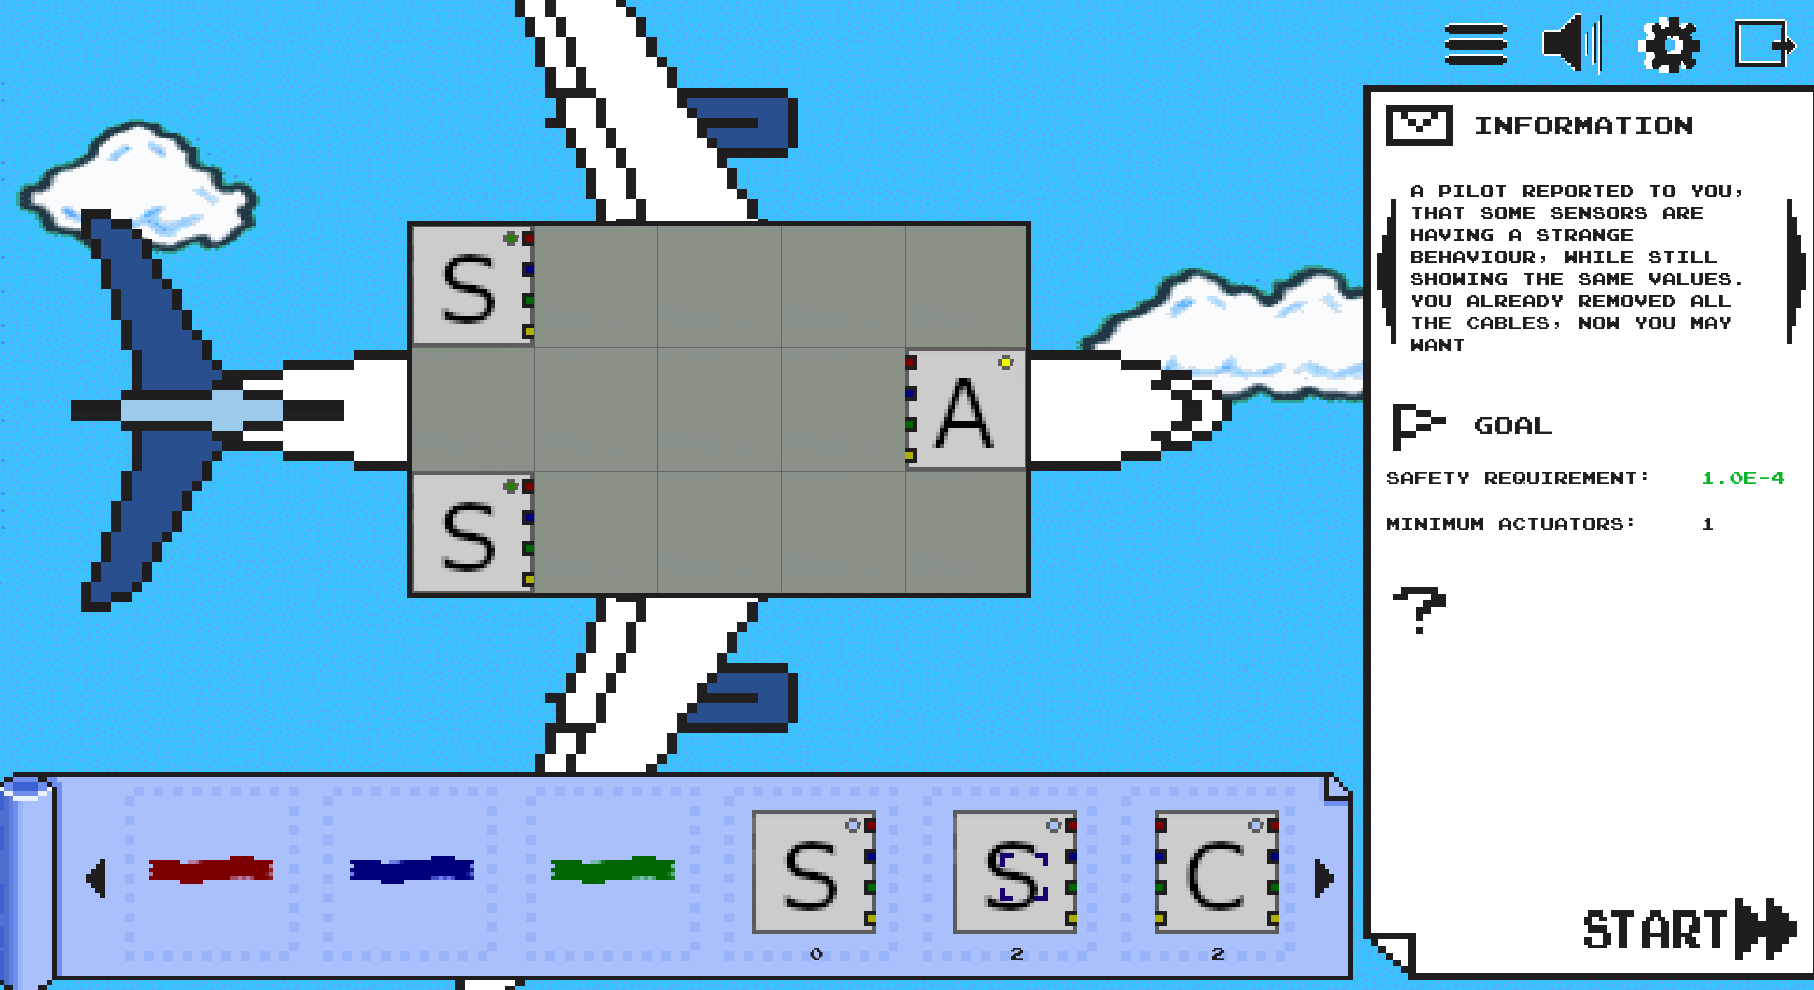
\includegraphics[width=\textwidth]{Pictures/res/implementation/scenes/cmf}
    \caption{Multiple useable sensors to visualize common mode failures}
    \label{fig:common-mode-scene}
\end{figure}
\begin{figure}
    \centering
    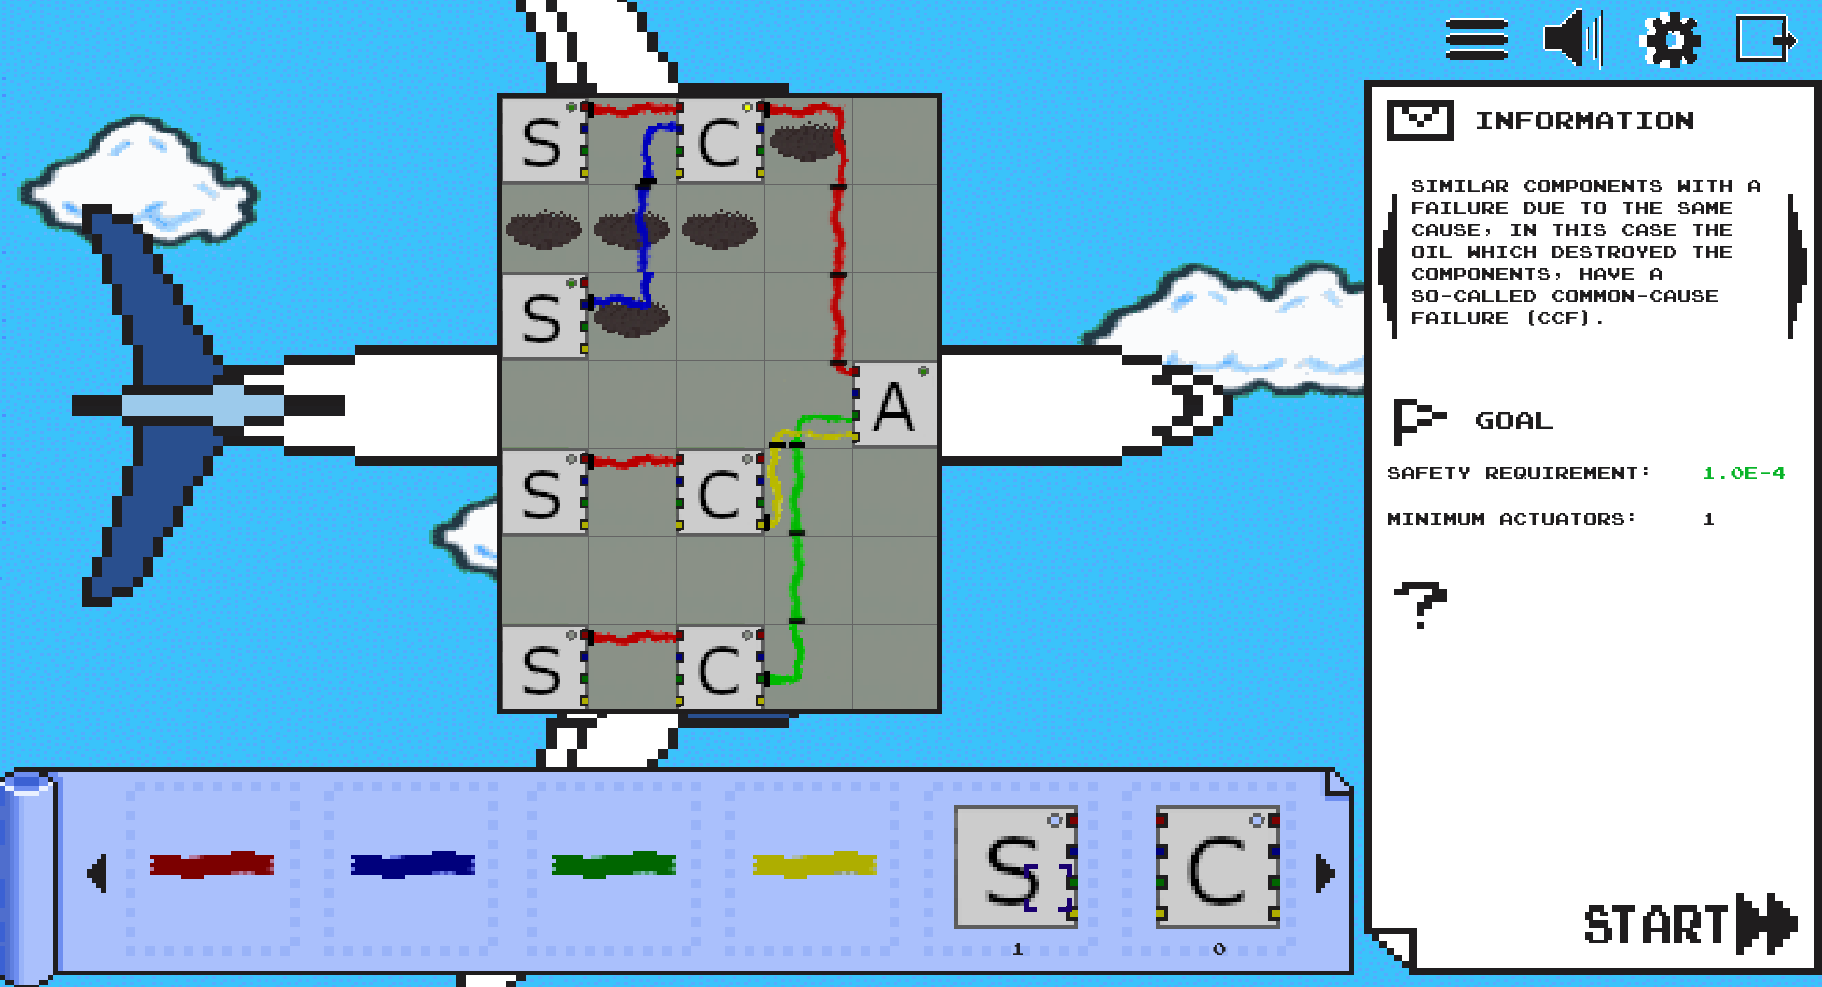
\includegraphics[width=\textwidth]{Pictures/res/implementation/scenes/oil-leak}
    \caption{A scene with an oil leakage on one side of the system to visualize common cause failures}
    \label{fig:common-cause-scene}
\end{figure}

For the game grid, tile sets as explained in section~\ref{subsec:tileset} are used, which consist of different seamless images for each of the
components, backgrounds and placeholders.
Figure~\ref{fig:tileset} shows all tiles that are currently available to the game implementation.
This is easily extendable by adding more tiles to the set, which may be used for backgrounds, placeholders or new simulation entities.
\begin{figure}
    \centering
    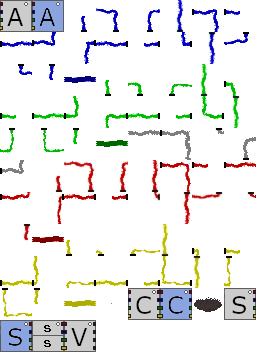
\includegraphics[width=\textwidth]{Pictures/res/implementation/tileset}
    \caption{Tileset}
    \label{fig:tileset}
\end{figure}

\subsubsection{Tutorial Scenes}\label{subsubsec:tutorial-scenes}
To elucidate the gameplay, tutorial dialogues have been incorporated into select scenes of the game.
To ensure that these dialogues are captivating and engaging, characters were crafted to make the tutorials more interactive.
The character models employed in the implementation can be seen in figure~\ref{fig:character-models}.
This framework is easily expandable, allowing for the addition of more characters to develop further tutorials,
dialogues, or even a storyline in the future, utilizing these character designs.
\begin{figure}
    \centering
    
\includegraphics[width=\textwidth]{Pictures/res/implementation/character-models}
    \caption{Character Models (left to right): Tina Technician, Ingo Engineer, Pete Pilot}
    \label{fig:character-models}
\end{figure}

\section{Data Storage \& Data Parsing}\label{sec:data-storage-&-data-parsing}
It was chosen to save and load resources from XML files, due to the benefits of this file format.
XML means \textit{eXtensible Markup Language}, and is a markup language that is used for encoding documents in a format that is easily readable for both human and computers.
It was designed to be flexible and extensible, allowing developers to create their own markup tags and structure data in a way that is specific to their needs~\cite{xml}.
\\
XML documents are made up of elements, which are enclosed in opening and closing tags, and attributes, which provide additional information about the element.
The structure of an XML document is defined by a \textit{Document Type Definition (DTD)} or an \textit{XML Schema}, which specifies the elements and attributes that are allowed in the document and the relationships between them.
\\
One of the main benefits of XML is its ability to store and transfer data in a standardized format that can be easily parsed by different software applications, regardless of the platform, and there are
already multiple implementations available to successfully do this, including JAVA's built-in library for DOM parsing~\cite{dom-parser}.
\\
The structure of the different XML files for levels, tilesets, scores and language used in this project will be explained in the next chapters.
\subsection{Tileset}\label{subsec:tileset}
A tileset file contains a list of multiple tile nodes, which each have an id and a type attribute.
A tile always contains exactly one image node, which has at least width, height and a resource path to an image assigned to it.
Optionally, there can also be a description attribute which can be used to set a tooltip that will be rendered to the games tooltip panel, if available.
\\
The code snippet shown in figure~\ref{fig:xml-tileset} shows a tileset with a single tile of the type Computer, including its description and image parameters.
\\ \\
\begin{figure}
\begin{lstlisting}[language=XML,label={lst:tileset-xml}]
    <?xml version="1.0" encoding="UTF-8"?>
    <tileset name="tiles">
        <tile id="200" type="COMPUTER">
            <image width="32" height="32" source="res/avionics/default.png" description="Default CPU Component"/>
        </tile>
    </tileset>
\end{lstlisting}
    \caption{XML Schema of the tileset file}
    \label{fig:xml-tileset}
\end{figure}
\subsection{Level Files}\label{subsec:level-files}
The root node of a level structure is the map node, which always includes attributes for assigning an id, a name,
a difficulty level (tutorial, easy, medium, hard, or custom), and grid dimensions (width and height) for the game grid.
The map node consists of a sub node for descriptions (and description parts, if the text should be divided into multiple displayable segments),
a sub node for available building elements from the build panel, and a sub node defining the pre-existing objects on the grid.
\\
Moreover, the goal and goal definition sub-nodes provide information on the criteria for completing a level (e.g.,
safety requirements, minimum components that must function correctly, and maximum out-of-control components).
The tileset used by the map must be specified in the tileset sub node,
and level unlocks (e.g., which level ids become accessible after completing the current level) can also be defined.
\\
The code snippet shown in figure~\ref{fig:xml-level} demonstrates an example of the level XML file structure, which depicts a 5x3 game grid with one actuator at position $x = 4$ and $y = 1$,
and two sensors at positions $x = 0$ and $y = [0, 2]$.
\\
It is important to note that the width and height attributes represent the actual map size, similar to the length of an array in Java,
while the positions indicate the grid positions starting at 0, akin to indexes in Java arrays.
\begin{figure}
\begin{lstlisting}[language=XML,label={lst:level-xml}]
    <?xml version="1.0" encoding="UTF-8"?>
    <map id="0" name="@0" width="5" height="3" difficulty="EASY">
        <description>
            <part>@1</part>
        </description>
        <goal>1e-7</goal>
        <goalDefinition workingActuators="1" workingSensors="0" workingComputers="0"/>
        <tileset source="base_tiles.xml"/>
        <unlocks>
            <unlock>6</unlock>
        </unlocks>
        <build>
            <entity id="500" amount="1000" safety="0" correctSignalsNeeded="1" outOfControlSignalsAccepted="0"/>
            <entity id="501" amount="1000" safety="0" correctSignalsNeeded="1" outOfControlSignalsAccepted="0"/>
            <entity id="502" amount="1000" safety="0" correctSignalsNeeded="1" outOfControlSignalsAccepted="0"/>
            <entity id="203" amount="2" safety="0" failureDetectionRatio="1" correctSignalsNeeded="1"
                    outOfControlSignalsAccepted="0"/>
        </build>
        <layer id="0" name="Tile Layer 1">
            <entity x="0" y="0" id="201" interactable="false" safety="1e-4" failureDetectionRatio="1"
                    correctSignalsNeeded="0" outOfControlSignalsAccepted="0"/>
            <entity x="0" y="2" id="201" interactable="false" safety="1e-4" failureDetectionRatio="1"
                    correctSignalsNeeded="0" outOfControlSignalsAccepted="0"/>
            <entity x="4" y="1" id="205" interactable="false" safety="0" failureDetectionRatio="1" correctSignalsNeeded="2"
                    outOfControlSignalsAccepted="0"/>
        </layer>
    </map>
\end{lstlisting}
    \caption{XML Schema of a level file}
    \label{fig:xml-level}
\end{figure}
\subsection{Language Files}\label{subsec:language-files}
A language file, as displayed in figure~\ref{fig:xml-lang} contains all text content used in the game for a specified language.
In the root node, the language type can be given according to the IETF language tag \todo{add source}, if supported by the game (i.e.\ implemented in the language manager).
Within this root node, string nodes are created which contain the id of a string as an attribute and the actual content as text.
Each of the ids has to be unique, otherwise only the first specified id will be considered in the implementation.
\\
\begin{figure}
\begin{lstlisting}[language=XML,label={lst:lang-xml}]
    <strings language="DE_DE">
        <string id="1">Sample Text</string>
    </strings>
\end{lstlisting}
    \caption{XML Schema of a language file}
    \label{fig:xml-lang}
\end{figure}

\subsection{Score Files}\label{subsec:score-files}
Highscores for each level are saved in a separate xml file containing information about the profile name, score and level id.
The schema shown in figure~\ref{fig:xml-score} is used for this file, saving the score 91 for a user who played level id one.
\\
\begin{figure}
\begin{lstlisting}[language=XML,label={lst:score-xml}]
    <scores>
      <scoreItem>
        <name>User</name>
        <score>91</score>
        <level>1</level>
      </scoreItem>
    </scores>
\end{lstlisting}
    \caption{XML schema of a score file}
    \label{fig:xml-score}
\end{figure}

\subsection{Parsing}\label{subsec:parsing}
For data parsing, a standard DOM parser library provided by Java is used.
It handles all possible exception types, such as input exceptions or malformed xml documents by default, which are added to the log of the game
and allows for a quick setup of parsing
the necessary nodes, attributes and text contents from the given input files.
As each type of file handled by default for this game has a different structure, the ResourceManager and its sub managers implement methods to handle
each file structure: loading a level, loading a tileset, loading scores, loading language data and loading fonts.

\section{External Device Inputs}\label{sec:external-device-inputs}
Since the game developed within the scope of this project is primarily intended for a younger audience at public events,
it was essential to accommodate not just mouse and keyboard inputs, but also gamepads.
This is because gamepads contribute to a more game-like atmosphere for users, while avoiding possible wrong inputs made by
other peripherals that can not be processed by the game.
This chapter will discuss the integration of gamepads, including game controllers, into the game.
\subsection{Mouse \& Keyboard}\label{subsec:mouse-&-keyboard}
The standard input device for the game are mouse and keyboard.
\subsection{Gamepad Integration}\label{subsec:gamepad-integration}
For gamepad integration, the open source library \textit{Jamepad} is used.
It automatically detects most USB controller devices and has an inbuilt button mapping which can be used in the implementation.
A separate thread captures game pad inputs, as actions may occur in between the calculated frames of the game engine.
Button handling is implemented in a way that a button press creates a new mouse event and the cursor position which is then handled by the action
systems' mouse event handling method.
This reduces maintenance and new implementation of buttons and actions, while being guaranteed to work correctly with all devices.
The game may also be played without a gamepad, however it is recommended to use the gamepad at least during public events.

\chapter{Results}\label{ch:results}
\section{Educational Achievements}\label{sec:educational-achievements}
\section{Limitations}\label{sec:limitations}
The field of aircraft system engineering is vast and intricate, and this work aims to simplify this complex subject by narrowing its scope.
Various failure types (such as mechanical or electrical failures) are considered only as a generalized failure of any type.
However, different failures may result in diverse system behaviors, which must be analyzed in real-life situations.
\\
While incorporating multiple failure types could be a potential future feature, it would considerably slow down the current
approach of Markov generation, as explained in~\ref{subsubsec:example-markov-chains}.
The implementation is based on generating Markov chains that grow in size as the number of components in the system increases.
Introducing multiple failure types would further raise the complexity of the Markov chain, resulting in approximately $m^n$ more states,
where $m$ represents the number of distinct failure states and $n$ the number of components.
\todo{check if that is true, adapt equations}

\section{Challenges}\label{sec:challenges}
During the implementation process, some major challenges - not only negative, also in a positive way - occurred, which will be described in this chapter, to give an
overview and a guideline on what may be done differently during the next iteration of the project or during the development of other
applications and what may be done in a similar way, as it worked well.
\subsection{Game Engine Development}\label{subsec:entity-component-system-challenges}
One major part of this work was the implementation of a game engine, using the entity-component system approach in a similar way
Unity handles its GameObjects.
This resulted in a very structured and extendable framework, which servers as a good baseline and enables the development of the actual game.
As much as this provides flexibility, it is also a lot of work that went into a part of the implementation, that to the user
does not provide any obvious benefits, as there is nothing which is actually visible from this implementation approach.
However, the new implementation of a game engine was ultimately chosen due to the overwhelming amount of features and complexity
already existing game engines provide, where only a very small subset would be used for developing the actual game, and other problems
may have occurred due to the relatively specific use case of this work.
Eventually, finishing the work with a game engine that can be used for any further developments of the game without having to worry
about the implementation of the engine is a benefit especially for further development and feature implementations.

\subsection{Programming Language}\label{subsec:programming-language}
Another challenge was the usage of Java itself, as this was mainly chosen due to already existing coding knowledge with this
language and a great availability of already existing libraries, such as rendering libraries.
Furthermore, Java is a very understandable and readable language and applications can easily be used on most devices, which are great benefits.
However, other languages such as C++ or C\# may be more suitable for game development in general, which is not only shown by
the usage of languages in the modern gaming industry (e.g. Minecraft was originally created in Java, but is now also switching to C++), but
also by the general performance of methods.
Due to Java being interpreted, most methods, in this work this is especially mentionable for the simulation part of the game, are being slowed down
by a margin compared to other languages like C++.
To correctly assess this, these methods would also need to be implemented in other languages, however the above-mentioned would
be the expected result.
\chapter{Conclusion \& Prospects}\label{ch:conclusion-&-prospects}
In conclusion, this thesis has presented the development of a gamified simulation of safety relevant aircraft systems.
The motivation for this work was to provide a novel approach to gaining attention and interest for the topic of aircraft
system engineering, specifically at the University of Stuttgart, by combining an engaging and fun experience of gaming and the
informative content of basic system engineering concepts in aviation.
\\
The main contributions to this work are the conceptualization and development of a game engine that is used to
design and implement a game by using it.
Different scenarios are implemented to give insight into a range of different concepts, such as redundancy or different failure types in an
interactive environment for the target audience of younger children, teenagers or families to gain interest in a playful way.
The game itself uses a simplified simulation approach in the backend by using the Markov method to generate and simulate failure states
across the system in a way, that is also used in safety analysis of aircraft systems.
\\
The game engine follows a modular entity component system architecture, which enables flexible, maintainable and highly customizable
development of game entities and game behaviors.
This also allows for further development of the game and easy integration of new concepts, components, scenarios and logics.
Therefore, the game and its engine serve as a baseline to any further requirements that are made to further improve the experience of the game.
\\
As the first time this game is going to be presented to the public is the ``Tag der Wissenschaft'' at the University of Stuttgart, which is happening
on 13th of May 2023, there may be feedback which can be implemented in the game afterwards.
In case any misunderstandings happen during play-throughs of different levels or any bugs occur, that were not found during testing of
the application, a documentation of the former mentioned feedbacks should be helpful to give a guideline on any improvements that may be made.
\\
Additionally, it would be interesting to integrate a 2 player mode, which could either be cooperative in a way, that two players
try to build a system together, or competitive, where the screen can be split and a further factor for the score calculation may be added in the time difference
needed for each player to finish the game.
\\
As more people get involved in playing the game, this work serves as a basis for any further research, development and use-case integration in the area
of game-based learning and as a demonstrator game, which can contribute to making people interested in learning more about the topic and is possibly and effective
approach to gain future students and therefore future engineers in the field of aircraft system engineering.

%% ============================================================
%%  ***  Bibliography
%% ============================================================
\normalem	% Entfernt Unterstrich des Titels
\printbibliography[heading=bibintoc,title=Bibliography] %Literaturverzeichnisse ausgeben

%% ============================================================
%%  ***  Appendix
%% ============================================================
\appendix
% Seitennummerierung wird geändert
\pretocmd{\chapter}{%
	\cleardoublepage
	\pagenumbering{arabic}%
	\renewcommand*{\thepage}{\thechapter\arabic{page}}%
}{}{}
%\chapter{Anhang}
\label{app:A}

Beim Aufbau einer Diplomarbeit oder Bachelorarbeit ist der Anhang kein Sammelbecken für alles Übriggebliebene, das im Rahmen der Arbeit gesammelt wurde und für die Bearbeitung der Arbeit nicht relevant war.

In den Anhang gehören die Materialien, die nicht zwingend für das Textverständnis erforderlich sind. Berechnungen, deren Ergebnisse im Text verwendet wurden, oder der Arbeit zugrundeliegende Fragebögen können hier ausführlicher dargestellt werden .

\chapter{Tabelle Landscape}\label{app:tabelle-landscape}




\begin{landscape}


%	\begin{singlespacing}
\begin{table}[h]	
%		\begingroup
		\footnotesize
		\setlength\tabcolsep{2pt}
		\tabulinesep=1mm
%%		\renewcommand{\arraystretch}{1.4}
%		
	\begin{tabu} to 1.4\textheight{X[l,m,12]X[l,m,4]|X[r,m,10]X[r,m,10]|X[r,m,10]X[r,m,10]|X[r,m,10]X[r,m,10]|X[r,m,10]X[r,m,10]|X[r,m,10]X[r,m,10]|X[r,m,10]X[r,m,10]|X[r,m,10]X[r,m,10]|X[r,m,10]X[r,m,10]|X[r,m,10]X[r,m,10]}
		\hline
		a & a & a & a & a & a & a & a & a & a & a & a & a & a & a & a & a & a & a & a\\\hline
%%% Header %%%%% 
\toprule
\toprule
%
\multicolumn{2}{c|}{Control} & \multicolumn{2}{c|}{load var 1} & \multicolumn{2}{c|}{load var 2} & \multicolumn{2}{c|}{load var 3} & \multicolumn{2}{c|}{load var 4} & \multicolumn{2}{c|}{load var 9} & \multicolumn{2}{c|}{load var 10} & \multicolumn{2}{c|}{load var 13} & \multicolumn{2}{c|}{load var 14} & \multicolumn{2}{c}{overall longitudinal} \\
\multicolumn{2}{c|}{Surface}  & max. defl. & min. defl. & max. defl. & min. defl. & max. defl. & min. defl. & max. defl. & min. defl. & max. defl. & min. defl. & max. defl. & min. defl. & max. defl. & min. defl. & max. defl. & min. defl. & max. defl. & min. defl. \\
%
\midrule
%
%\endhead
%%%%%%%%%%%%%%%%%
%\bottomrule
%\bottomrule
%\endfoot
%%%%%%%%%%%%%%%%
%\hline
%\endlastfoot
%%%%%%%%%%%%%%%%%%%%%%%%%%%%%%%%%%%%%%%%%%%%%%%%%%%%%%%%%%%%%%%%%%
%
%
\multirow{10}{10mm}{right wing} & 1     & 3.1   & -15.7 & 21.0  & -3.9  & 8.7   & -7.1  & 7.1   & -8.7  & 8.0   & -9.7  & 12.9  & -10.2 & 4.4   & -3.1  & 3.4   & -4.4  & 21.0  & -15.7 \\
      & 2     & 3.1   & -15.7 & 21.0  & -3.9  & 8.7   & -7.1  & 7.1   & -8.7  & 8.0   & -9.7  & 12.9  & -10.2 & 4.4   & -3.0  & 3.3   & -4.4  & 21.0  & -15.7 \\
      & 3     & 0.1   & -0.2  & 0.3   & -0.2  & 0.2   & -0.2  & 0.2   & -0.2  & 2.5   & -16.2 & 21.6  & -3.4  & 0.2   & -0.2  & 0.2   & -0.2  & 21.6  & -16.2 \\
      & 4     & 0.1   & -0.2  & 0.3   & -0.2  & 0.2   & -0.2  & 0.2   & -0.2  & 2.5   & -16.2 & 21.6  & -3.4  & 0.2   & -0.2  & 0.2   & -0.2  & 21.6  & -16.2 \\
      & 5     & 18.4  & -25.0 & 25.0  & -25.0 & 25.0  & -19.8 & 19.8  & -25.0 & 0.8   & -25.0 & 25.0  & -1.0  & 11.5  & -10.6 & 10.6  & -11.1 & 25.0  & -25.0 \\
      & 6     & 0.0   & 0.0   & 0.0   & 0.0   & 0.0   & 0.0   & 0.0   & 0.0   & 0.0   & 0.0   & 0.0   & 0.0   & 0.0   & 0.0   & 0.0   & 0.0   & 0.0   & 0.0 \\
      & 7     & 0.0   & 0.0   & 0.0   & 0.0   & 0.0   & 0.0   & 0.0   & 0.0   & 0.0   & 0.0   & 0.0   & 0.0   & 0.0   & 0.0   & 0.0   & 0.0   & 0.0   & 0.0 \\
      & 8     & 1.7   & -0.9  & 1.2   & -2.3  & 1.8   & -2.6  & 2.6   & -1.8  & 1.4   & -1.7  & 2.2   & -1.9  & 2.1   & -2.0  & 1.9   & -2.1  & 2.6   & -2.6 \\
      & 9     & 0.0   & 0.0   & 0.0   & 0.0   & 0.0   & 0.0   & 0.0   & 0.0   & 0.0   & 0.0   & 0.0   & 0.0   & 4.3   & 0.0   & 3.5   & 0.0   & 4.3   & 0.0 \\
      & 10    & 0.0   & 0.0   & 0.0   & 0.0   & 0.0   & 0.0   & 0.0   & 0.0   & 0.0   & 0.0   & 0.0   & 0.0   & 0.0   & 0.0   & 0.0   & 0.0   & 0.0   & 0.0 \\
\midrule
\multirow{10}{10mm}{left wing} & 1     & 3.1   & -15.7 & 21.0  & -3.9  & 8.7   & -7.1  & 7.1   & -8.7  & 8.0   & -9.7  & 12.9  & -10.2 & 4.4   & -3.1  & 3.4   & -4.4  & 21.0  & -15.7 \\
      & 2     & 3.1   & -15.7 & 21.0  & -3.9  & 8.7   & -7.1  & 7.1   & -8.7  & 8.0   & -9.7  & 12.9  & -10.2 & 4.4   & -3.0  & 3.3   & -4.4  & 21.0  & -15.7 \\
      & 3     & 0.2   & -0.1  & 0.2   & -0.3  & 0.2   & -0.2  & 0.2   & -0.2  & 2.5   & -16.2 & 21.6  & -3.4  & 0.2   & -0.2  & 0.2   & -0.2  & 21.6  & -16.2 \\
      & 4     & 0.2   & -0.1  & 0.2   & -0.3  & 0.2   & -0.2  & 0.2   & -0.2  & 2.5   & -16.2 & 21.6  & -3.4  & 0.2   & -0.2  & 0.2   & -0.2  & 21.6  & -16.2 \\
      & 5     & 18.4  & -25.0 & 25.0  & -25.0 & 25.0  & -19.8 & 19.8  & -25.0 & 0.8   & -25.0 & 25.0  & -1.0  & 11.4  & -10.5 & 10.5  & -11.1 & 25.0  & -25.0 \\
      & 6     & 0.0   & 0.0   & 0.0   & 0.0   & 0.0   & 0.0   & 0.0   & 0.0   & 0.0   & 0.0   & 0.0   & 0.0   & 0.0   & 0.0   & 0.0   & 0.0   & 0.0   & 0.0 \\
      & 7     & 0.0   & 0.0   & 0.0   & 0.0   & 0.0   & 0.0   & 0.0   & 0.0   & 0.0   & 0.0   & 0.0   & 0.0   & 0.0   & 0.0   & 0.0   & 0.0   & 0.0   & 0.0 \\
      & 8     & 0.9   & -1.7  & 2.3   & -1.2  & 2.6   & -1.8  & 1.8   & -2.6  & 1.7   & -1.4  & 1.9   & -2.2  & 2.0   & -2.1  & 2.1   & -1.9  & 2.6   & -2.6 \\
      & 9     & 0.0   & 0.0   & 0.0   & 0.0   & 0.0   & 0.0   & 0.0   & 0.0   & 0.0   & 0.0   & 0.0   & 0.0   & 4.3   & 0.0   & 3.5   & 0.0   & 4.3   & 0.0 \\
      & 10    & 0.0   & 0.0   & 0.0   & 0.0   & 0.0   & 0.0   & 0.0   & 0.0   & 0.0   & 0.0   & 0.0   & 0.0   & 0.0   & 0.0   & 0.0   & 0.0   & 0.0   & 0.0 \\
\bottomrule
\bottomrule

\multicolumn{20}{l}{Control Functions:} \\
\multicolumn{20}{l}{Pitch: 1 \& 2; Roll: 3 \& 4; Stabilisation: 5; Spliteron: 6; Miniflap: 7; Rudder: 8; Inner Spoiler: 9; Outer Spoiler: 10} \\
\multicolumn{20}{l}{Note: The Control Surfaces 6 and 7 are not operational within the MATLAB SIMULINK models.} \\		
		\end{tabu}
\caption{Control surface deflections at longitudinal manoeuvres}\label{tab:Flap-Deflections}
\end{table}
%		\endgroup

%	\end{singlespacing}

\end{landscape}
\normalsize




\chapter{Mehrseitige Tabelle}\label{app:mehrsteige-tabelle}

\begin{longtabu} to \textwidth{|X[l,m,1]|X[l,m,1]|X[l,m,1]|}

	
	\toprule\toprule \multicolumn{1}{|c|}{\textbf{First column}} & \multicolumn{1}{c|}{\textbf{Second column}} & \multicolumn{1}{c|}{\textbf{Third column}} \\ \midrule 
	\endfirsthead
	
	\multicolumn{3}{c}%
	{\tablename\ \thetable{} -- continued from previous page} \\
	\toprule\toprule \multicolumn{1}{|c|}{\textbf{First column}} & \multicolumn{1}{c|}{\textbf{Second column}} & \multicolumn{1}{c|}{\textbf{Third column}} \\ \midrule 
	\endhead
	
	\midrule \multicolumn{3}{|r|}{{Continued on next page}} \\ \bottomrule\bottomrule
	\caption[]{A sample long table} \label{tab:long} \\
	\endfoot
	
	\bottomrule
	\bottomrule
	\caption[A sample long table]{A sample long table} \label{tab:long} \\
	\endlastfoot
	
	One & abcdef ghjijklmn & 123.456778 \\
	One & abcdef ghjijklmn & 123.456778 \\
	One & abcdef ghjijklmn & 123.456778 \\
	One & abcdef ghjijklmn & 123.456778 \\
	One & abcdef ghjijklmn & 123.456778 \\
	One & abcdef ghjijklmn & 123.456778 \\
	One & abcdef ghjijklmn & 123.456778 \\
	One & abcdef ghjijklmn & 123.456778 \\
	One & abcdef ghjijklmn & 123.456778 \\
	One & abcdef ghjijklmn & 123.456778 \\
	One & abcdef ghjijklmn & 123.456778 \\
	One & abcdef ghjijklmn & 123.456778 \\
	One & abcdef ghjijklmn & 123.456778 \\
	One & abcdef ghjijklmn & 123.456778 \\
	One & abcdef ghjijklmn & 123.456778 \\
	One & abcdef ghjijklmn & 123.456778 \\
	One & abcdef ghjijklmn & 123.456778 \\
	One & abcdef ghjijklmn & 123.456778 \\
	One & abcdef ghjijklmn & 123.456778 \\
	One & abcdef ghjijklmn & 123.456778 \\
	One & abcdef ghjijklmn & 123.456778 \\
	One & abcdef ghjijklmn & 123.456778 \\
	One & abcdef ghjijklmn & 123.456778 \\
	One & abcdef ghjijklmn & 123.456778 \\
	One & abcdef ghjijklmn & 123.456778 \\
	One & abcdef ghjijklmn & 123.456778 \\
	One & abcdef ghjijklmn & 123.456778 \\
	One & abcdef ghjijklmn & 123.456778 \\
	One & abcdef ghjijklmn & 123.456778 \\
	One & abcdef ghjijklmn & 123.456778 \\
	One & abcdef ghjijklmn & 123.456778 \\
	One & abcdef ghjijklmn & 123.456778 \\
	One & abcdef ghjijklmn & 123.456778 \\
	One & abcdef ghjijklmn & 123.456778 \\
	One & abcdef ghjijklmn & 123.456778 \\
	One & abcdef ghjijklmn & 123.456778 \\
	One & abcdef ghjijklmn & 123.456778 \\
	One & abcdef ghjijklmn & 123.456778 \\
	One & abcdef ghjijklmn & 123.456778 \\
	One & abcdef ghjijklmn & 123.456778 \\
	One & abcdef ghjijklmn & 123.456778 \\
	One & abcdef ghjijklmn & 123.456778 \\
	One & abcdef ghjijklmn & 123.456778 \\
	One & abcdef ghjijklmn & 123.456778 \\
	One & abcdef ghjijklmn & 123.456778 \\
	One & abcdef ghjijklmn & 123.456778 \\
	One & abcdef ghjijklmn & 123.456778 \\
	One & abcdef ghjijklmn & 123.456778 \\
	One & abcdef ghjijklmn & 123.456778 \\
	One & abcdef ghjijklmn & 123.456778 \\
	One & abcdef ghjijklmn & 123.456778 \\
	One & abcdef ghjijklmn & 123.456778 \\
	One & abcdef ghjijklmn & 123.456778 \\
	One & abcdef ghjijklmn & 123.456778 \\
	One & abcdef ghjijklmn & 123.456778 \\
	One & abcdef ghjijklmn & 123.456778 \\
	One & abcdef ghjijklmn & 123.456778 \\
	One & abcdef ghjijklmn & 123.456778 \\
	One & abcdef ghjijklmn & 123.456778 \\
	One & abcdef ghjijklmn & 123.456778 \\
	One & abcdef ghjijklmn & 123.456778 \\
	One & abcdef ghjijklmn & 123.456778 \\
	One & abcdef ghjijklmn & 123.456778 \\
	One & abcdef ghjijklmn & 123.456778 \\
	One & abcdef ghjijklmn & 123.456778 \\
	One & abcdef ghjijklmn & 123.456778 \\
	One & abcdef ghjijklmn & 123.456778 \\
	One & abcdef ghjijklmn & 123.456778 \\
	One & abcdef ghjijklmn & 123.456778 \\
	One & abcdef ghjijklmn & 123.456778 \\
	One & abcdef ghjijklmn & 123.456778 \\
	One & abcdef ghjijklmn & 123.456778 \\
	One & abcdef ghjijklmn & 123.456778 \\
	One & abcdef ghjijklmn & 123.456778 \\
	One & abcdef ghjijklmn & 123.456778 \\
	One & abcdef ghjijklmn & 123.456778 \\
	One & abcdef ghjijklmn & 123.456778 \\
	One & abcdef ghjijklmn & 123.456778 \\
	One & abcdef ghjijklmn & 123.456778 \\
	One & abcdef ghjijklmn & 123.456778 \\
\end{longtabu}
\end{document}
